% Options for packages loaded elsewhere
\PassOptionsToPackage{unicode}{hyperref}
\PassOptionsToPackage{hyphens}{url}
%
\documentclass[
]{book}
\usepackage{amsmath,amssymb}
\usepackage{iftex}
\ifPDFTeX
  \usepackage[T1]{fontenc}
  \usepackage[utf8]{inputenc}
  \usepackage{textcomp} % provide euro and other symbols
\else % if luatex or xetex
  \usepackage{unicode-math} % this also loads fontspec
  \defaultfontfeatures{Scale=MatchLowercase}
  \defaultfontfeatures[\rmfamily]{Ligatures=TeX,Scale=1}
\fi
\usepackage{lmodern}
\ifPDFTeX\else
  % xetex/luatex font selection
\fi
% Use upquote if available, for straight quotes in verbatim environments
\IfFileExists{upquote.sty}{\usepackage{upquote}}{}
\IfFileExists{microtype.sty}{% use microtype if available
  \usepackage[]{microtype}
  \UseMicrotypeSet[protrusion]{basicmath} % disable protrusion for tt fonts
}{}
\makeatletter
\@ifundefined{KOMAClassName}{% if non-KOMA class
  \IfFileExists{parskip.sty}{%
    \usepackage{parskip}
  }{% else
    \setlength{\parindent}{0pt}
    \setlength{\parskip}{6pt plus 2pt minus 1pt}}
}{% if KOMA class
  \KOMAoptions{parskip=half}}
\makeatother
\usepackage{xcolor}
\usepackage[a4paper,margin=2.5cm]{geometry}
\usepackage{longtable,booktabs,array}
\usepackage{calc} % for calculating minipage widths
% Correct order of tables after \paragraph or \subparagraph
\usepackage{etoolbox}
\makeatletter
\patchcmd\longtable{\par}{\if@noskipsec\mbox{}\fi\par}{}{}
\makeatother
% Allow footnotes in longtable head/foot
\IfFileExists{footnotehyper.sty}{\usepackage{footnotehyper}}{\usepackage{footnote}}
\makesavenoteenv{longtable}
\usepackage{graphicx}
\makeatletter
\def\maxwidth{\ifdim\Gin@nat@width>\linewidth\linewidth\else\Gin@nat@width\fi}
\def\maxheight{\ifdim\Gin@nat@height>\textheight\textheight\else\Gin@nat@height\fi}
\makeatother
% Scale images if necessary, so that they will not overflow the page
% margins by default, and it is still possible to overwrite the defaults
% using explicit options in \includegraphics[width, height, ...]{}
\setkeys{Gin}{width=\maxwidth,height=\maxheight,keepaspectratio}
% Set default figure placement to htbp
\makeatletter
\def\fps@figure{htbp}
\makeatother
\setlength{\emergencystretch}{3em} % prevent overfull lines
\providecommand{\tightlist}{%
  \setlength{\itemsep}{0pt}\setlength{\parskip}{0pt}}
\setcounter{secnumdepth}{5}
\usepackage{booktabs}
\usepackage{luatexja}
\usepackage{luatexja-fontspec}
\setmainjfont{IPAGothic}
\setsansjfont{IPAGothic}
\usepackage{booktabs}
\usepackage{longtable}
\usepackage{array}
\usepackage{multirow}
\usepackage{wrapfig}
\usepackage{float}
\usepackage{colortbl}
\usepackage{pdflscape}
\usepackage{tabu}
\usepackage{threeparttable}
\usepackage{threeparttablex}
\usepackage[normalem]{ulem}
\usepackage{makecell}
\usepackage{xcolor}
\ifLuaTeX
  \usepackage{selnolig}  % disable illegal ligatures
\fi
\usepackage[]{natbib}
\bibliographystyle{apalike}
\IfFileExists{bookmark.sty}{\usepackage{bookmark}}{\usepackage{hyperref}}
\IfFileExists{xurl.sty}{\usepackage{xurl}}{} % add URL line breaks if available
\urlstyle{same}
\hypersetup{
  pdftitle={比較経営論},
  pdfauthor={飯島高雄},
  hidelinks,
  pdfcreator={LaTeX via pandoc}}

\title{比較経営論}
\author{飯島高雄}
\date{2023-08-21}

\begin{document}
\maketitle

{
\setcounter{tocdepth}{1}
\tableofcontents
}
\hypertarget{intro}{%
\chapter{はじめに}\label{intro}}

\begin{itemize}
\item
  経営の目的やその機能は世界共通ですが、実際の経営手法というものは、経済・政治・社会・文化といった外部要因(環境)に大きく影響されます。

  \begin{itemize}
  \item
    そのため、世界各国で通用する唯一の「最適な経営手法」というものは存在しません。
  \item
    各国の状況にあった形で、各国バージョンの「最適な経営手法」が存在します。
  \end{itemize}
\item
  本講義では、日本企業の経営システムとアメリカ企業およびアジア各国企業の経営システムを比較し、それぞれの特徴を整理し、その類似点および相違点を理解できるようになることを目指します。
\item
  本講義の内容を理解することで、以下の点について自分なりの意見が持てるようになります。

  \begin{itemize}
  \item
    外国企業の経営成功事例を無条件に取り入れるのは正しいといえるか?
  \item
    日本企業が海外進出したとき、現地子会社に日本的経営を求めるのは正しいといえるか?
  \item
    日本企業の経営システムは、世界的に見て特殊なのか?
  \end{itemize}
\item
  本講義の構成は、以下のとおりです。

  \begin{itemize}
  \item
    \ref{intro}では、本講義の目的と目標を提示します。
  \item
    \ref{management}は、\ref{usa}以降で使用する経営システムの比較基準を整理します。
  \item
    \ref{usa}では、アメリカ企業の経営システムを、外部要因(文化・政治・経済)・経営者・マネジメントの観点から考察します。
  \item
    \ref{japan}では、日本企業の経営システムを、外部要因(文化・政治・経済)・経営者・マネジメントの観点から考察します。
  \item
    \ref{asia}では、アジア企業の経営システムを、外部要因(文化・政治・経済)・経営者・マネジメントの観点から考察します。
  \item
    \ref{appendix}では、各国の経営システムの理解を深める諸項目を補足解説します。
  \end{itemize}
\end{itemize}

\hypertarget{comparizon}{%
\section{外国企業との比較}\label{comparizon}}

\begin{itemize}
\item
  本講義では、外国企業としてアメリカ企業とアジア企業を取り上げます。

  \begin{itemize}
  \tightlist
  \item
    一口にアジア企業といっても、中国企業、韓国企業、台湾企業など各国企業のマネジメントは異なりますが、日本と比較することを目的に「アジアとしての共通点」を中心に考えていきます。\\
  \end{itemize}
\item
  日本企業をアメリカ企業だけでなく、アジア企業とも比較するのには理由があります。(参考:池尾・黄・飯島 (2001), pp.~6-7)

  \begin{itemize}
  \item
    日本企業のマネジメントの特徴を本当に理解するためには、正反対の事例(アメリカはある意味で世界的に特異な経済です)と比較するだけで十分とはいえません。アメリカ企業にはみられないマネジメントでも、実はアジア企業には普遍的なものかも知れないからです。
  \item
    そこで日米比較に加えて、日本と近いと考えられる(必ずしもそうともいえないことがわかりますが・・・)アジア企業との比較が不可欠となります。
  \item
    このような多角的な比較を通じて、日本企業の特徴を「アメリカ企業との比較では異質であるが、アジア企業としては普遍的なもの」と「アジアの中でも異質であり、真に日本の特殊性といえるもの」に分類して理解することができます。
  \end{itemize}
\item
  比較として次の5つのパターンが考えられます。授業後の復習で、授業で解説した日本企業・アメリカ企業・アジア企業の特徴をこれらのパターンに整理してみてください。

  \begin{itemize}
  \item
    日本企業・アメリカ企業・アジア企業全てで共通(類似)する点
  \item
    日本企業とアメリカ企業は共通(類似)しているが、アジア企業は異なる点
  \item
    日本企業とアジア企業は共通(類似)しているが、アメリカ企業は異なる点
  \item
    アメリカ企業とアジア企業は共通(類似)しているが、日本企業は異なる点
  \item
    日本企業・アメリカ企業・アジア企業ぞれぞれが異なる点
  \end{itemize}
\end{itemize}

{\textbf{参考文献}}

池尾和人・黄圭燦・飯島高雄 (2001)『日韓経済システムの比較制度分析』日本経済新聞社.

\hypertarget{factor}{%
\section{マネジメントに影響を与える要因}\label{factor}}

\hypertarget{organizational-context}{%
\subsection{組織的文脈}\label{organizational-context}}

\begin{itemize}
\item
  企業(組織)は、売上、利益や生産性(効率)といった成果を上げるために活動しています。
\item
  その成果に影響を与えるのが、マネジメントのあり方(目的、プロセス、実践)です。つまり、マネジメントの良し悪しによって、企業の成果が異なってきます。
\item
  このマネジメントに影響を与える要因は\textbf{組織的文脈}といわれ、表 \ref{tab:factor} のように、外部要因と内部要因に分類できます。つまり、組織的文脈が異なると(望ましい)マネジメントのあり方も変わってきます。

  \begin{itemize}
  \item
    外部要因は企業が存立する環境(国・地域)によって決まるもので、同じ国の企業であればどの企業にとっても同じものです。
  \item
    内部要因は各企業で保有または設定するもので、同じ国の企業であっても企業ごとに異なります。
  \end{itemize}
\end{itemize}

\begin{table}

\caption{\label{tab:factor}組織的文脈}
\centering
\begin{tabular}[t]{l|l}
\hline
外部要因 & 内部要因\\
\hline
経済、政治・法、思想、技術、人口、社会、社会文化、教育、その他 & 組織目的、戦略、構造、資源、強み、弱み、経験、事業規模・範囲、成長速度、構成員の知識・熟練・経験・資質、組織文化、シナジー\\
\hline
\end{tabular}
\end{table}

出所)Edfelt (2010, p.12)

\hypertarget{common}{%
\subsection{各国企業の共通点}\label{common}}

\begin{itemize}
\item
  どの国の企業であっても共通(少なくとも類似)しているのは、内部要因にあたる組織(経営)目的です。
\item
  企業(株式会社)の経営目的は、どの国でも「企業価値の最大化」で共通しています。

  \begin{itemize}
  \tightlist
  \item
    \href{https://www.keidanren.or.jp/japanese/policy/2006/010/}{日本経済団体連合会 (2006, p.3)} は、次のように経営目的を示しています。
  \end{itemize}
\end{itemize}

\begin{quote}
ゴーイングコンサーンとしての企業の価値は、企業が将来にわたり生み出すことを期待されている付加価値の合計である。(中略)企業価値の最大化こそ経営者の使命であるが、近年、さまざまな次元で、企業価値の最大化に向けた経営戦略のあり方が議論の焦点となっている。
\end{quote}

\begin{itemize}
\tightlist
\item
  ただし、企業価値を誰に対してのものと考えるか(株主、債権者、従業員、顧客、取引先、地域住民、地球環境などのどこまでを含めるか)については、国や企業によって差があります\footnote{\href{https://plus.alc.co.jp/2018/01/meyer/}{他の国々との比較からあぶり出される日本文化の特徴やカルチャーマップの活かし方について}、著者がインタビューに答えています。}。
\end{itemize}

\begin{itemize}
\tightlist
\item
  \ref{basics} では内部要因に関連して、本講義で使用するマネジメントの基礎を復習します。
\end{itemize}

\hypertarget{difference}{%
\subsection{各国で相違が生じる背景}\label{difference}}

\begin{itemize}
\item
  「企業価値最大化」に至るプロセスは、国によって異なることがあります。

  \begin{itemize}
  \item
    それは、企業が存立する「地盤(外部要因)」が各国で異なるためです。「地盤」が異なれば、その上の「建物」の建て方も変わってくるというのと同じことです。
  \item
    \ref{hofstede}で取り上げる Hofstede (1993, pp.88-89)は、「すべての国に『マネジメント』と呼ばれるものがありますが、その意味は国によって多少異なり、そのプロセス、哲学、問題を理解するには、地域の状況についてかなりの歴史的および文化的洞察が必要です。(中略)マネジメントは、社会で起こっている他のプロセスから切り離すことができる現象ではありません」と述べています\footnote{この違いは思考法だけでなく、\protect\hyperlink{law}{法体系}の違いにも影響を与えています。}。
  \end{itemize}
\end{itemize}

\begin{itemize}
\item
  外部要因として、本講義では以下の3点から整理します。

  \begin{itemize}
  \item
    \ref{culture} で、本講義における比較で使用する文化についての比較基準を整理します。
  \item
    \ref{politics-and-law} で、本講義における比較で使用する法制度・政治システムについての分類を整理します。
  \item
    \ref{economy} で、本講義における比較で使用する経済システムについての分類を整理します。
  \end{itemize}
\item
  「企業価値最大化」に至るプロセスは、同じ国でも時代によって変化することがあります。

  \begin{itemize}
  \item
    時代が進むにつれて、人口・所得水準・技術水準などの外部要因が変化するためです。
  \item
    かつて優れたマネジメントとされたものが、その後の時代・環境の変化によって、その有効性が失われる(それどころか弊害になる)ということもあります。
  \end{itemize}
\end{itemize}

{\textbf{参考文献}}

Edfelt, Ralph B. (2010). Global Comparative Management. SAGE.

Hofstede, G. (1993). ``Cultural Constraints in Management Theories'' Academy of Management Executive. 7. 81-94.

\href{https://www.keidanren.or.jp/japanese/policy/2006/010/}{日本経済団体連合会 (2006)「企業価値の最大化に向けた経営戦略」}

\href{https://jp.ricoh.com/environment/report/index2014.html}{リコー (2014)「リコーグループサステナビリティレポート2014」}

\hypertarget{management}{%
\chapter{経営システムの比較基準}\label{management}}

\begin{itemize}
\item
  本章の構成は、以下のとおりです。

  \begin{itemize}
  \item
    \ref{basics}では、\ref{usa}以降で使用する経営システムの比較基準を整理します。
  \item
    \ref{culture}では、\ref{usa}以降で使用する外部要因として、文化の類型を整理します。
  \item
    \ref{politics-and-law}では、\ref{usa}以降で使用する外部要因として、政治体制や法制度の類型を整理します。
  \item
    \ref{economy}では、\ref{usa}以降で使用する外部要因として、経済システムの類型を整理します。
  \end{itemize}
\end{itemize}

\hypertarget{basics}{%
\section{マネジメントの基礎}\label{basics}}

\begin{itemize}
\item
  本節では、マネジメント理論の基礎を確認します。

  \begin{itemize}
  \item
    まず、経営学の源流として、\protect\hyperlink{taylor}{Taylorの科学的管理法}を復習します。
  \item
    次に、\protect\hyperlink{fayol}{Fayolの経営管理プロセス}を整理します。
  \end{itemize}
\end{itemize}

\hypertarget{taylor}{%
\subsection{Taylorの科学的管理法}\label{taylor}}

\begin{itemize}
\item
  経営学はおよそ100年前(20世紀初頭)に、実務家によって始まりました。

  \begin{itemize}
  \tightlist
  \item
    19世紀にアメリカは産業革命を経験し大量生産が可能になった反面、規模が拡大した企業をそれまでの「経験」や「勘」で経営することは難しくなったというのが、経営学が生まれた背景です。
  \end{itemize}
\item
  Taylor (1911)は、作業の効率(能率)を高めるために、科学的分析による作業の合理的な順序や作業量の設定、それに基づく生産の計画化や作業過程の効率的な管理方法をまとめました。

  \begin{itemize}
  \item
    製品1つ作るのにどういう動作をすべきか(標準動作)、1つの動作当りどのくらいの時間をかければよいか(標準工数)を設定し、そのことにより達成しうる仕事量(課業)を設定しました。
  \item
    従業員の評価は、課業(ノルマ)以上に達成した場合はボーナスを払い、課業に達しない者は、最初は注意、次に、訓告、戒告、そして最終的には解雇するようにしました。
  \item
    管理職も「計画」、「指揮」、「監督」と職能別に分け、1人に権限が集中しない組織を作りました。
  \end{itemize}
\end{itemize}

\begin{figure}
\includegraphics[width=240px]{https://upload.wikimedia.org/wikipedia/commons/thumb/b/b7/Frederick_Winslow_Taylor.JPG/298px-Frederick_Winslow_Taylor} \caption{Frederick Winslow Taylor}\label{fig:ftaylor}
\end{figure}

出所)\href{https://commons.wikimedia.org/wiki/File:Frederick_Winslow_Taylor.JPG}{Wikimedia Commons}

\begin{itemize}
\tightlist
\item
  三谷(2013, p.57)は、Taylorの科学的管理法について、以下のようにまとめています。
\end{itemize}

\begin{quote}
\textbf{「管理者による分析とマニュアルで生産性は上がる」}\\
- 作業生産性は時間・作業分析によって何倍にも上がり、作業環境の改善によっても上がる\\
- 人間は主に経済的動機によって動くので、段階的な賃率アップで動機づけるが、過重労働にならないように一定の最適労働量を定めるべき
\end{quote}

\begin{itemize}
\item
  科学的管理法は「機械的な考え」と批判もされましたが、経営学の原点として現代にも基本的な考え方として残っています。

  \begin{itemize}
  \item
    Mayoらは「客観的な労働条件」以上に「主観的な職場の人間関係」のほうが重要なのではないかという仮説に基づいて行った「ホーソン実験(Western Electric社のHawthorne工場における実験)」によって、Taylorの能率最優先・従業員の規律的な管理を軸とする「科学的管理法」に一石を投じました。
  \item
    三谷(2013, p.57)は、Mayoの人間関係論(的管理法)について、以下のようにまとめています。
  \end{itemize}
\end{itemize}

\begin{quote}
\textbf{「管理者と作業者の対話によって生産性は上がる」}\\
- 作業生産性は、テイラー的な作業環境より、作業者の士気(モラール)にもっとも左右される\\
- それ(=士気)は、職場の上司や同僚との人間関係や相互の信頼感(といった定性的なもの)によって決まる
\end{quote}

\begin{itemize}
\tightlist
\item
  チャップリンのモダンタイムスは、テイラー的な管理の風刺といえます。
\end{itemize}

\hypertarget{fayol}{%
\subsection{Fayolの経営管理プロセス}\label{fayol}}

\begin{itemize}
\item
  Taylorの関心が工場・現場の生産性(能率)向上を目的とした管理のあり方(management)であったのに対し、Fayolの関心は企業の経営管理のあり方(administration)にありました。

  \begin{itemize}
  \item
    Fayolの定義する「経営」:企業に委ねられた資源から最大限の利潤を引き出すように努力しながら、企業をその目的に向かって指導すること
  \item
    Fayolの定義する「管理」:経営がその進行を確保しなければならない6つの職能のうちの1つ
  \end{itemize}
\item
  Fayol (1916)は、経営を以下の6つの活動(職能)に分類しました。

  \begin{itemize}
  \item
    「1. 技術活動」は、工場など製品生産を担当する製造部、新製品(技術)開発を担当する研究開発部が該当します。
  \item
    「2. 商業活動」は、生産に必要な原材料購入を担当する資材部、製品を販売を担当する営業部が該当します。
  \item
    「3. 財務活動」は、企業経営に必要な資金の管理(調達と返済)を担当する財務部が該当します。
  \item
    「4. 保全活動」は、企業が保有する財産と従業員の保護・管理を担当する人事部や総務部が該当します。
  \item
    「5. 会計活動」は、製品原価や収益の計算を担当する経理部が該当します。
  \item
    「6. 管理活動」は、「1. 技術活動」から「5. 会計活動」までの各種活動間の調整、また企業戦略立案を担当する経営企画部が該当します。
  \item
    現場主任、部門長、経営陣と役職が上がるにつれて、「6. 管理活動」により多くの時間を費やすことになります。
  \end{itemize}
\end{itemize}

\begin{table}

\caption{\label{tab:fayola}Fayolによる活動(職能)分類}
\centering
\begin{tabular}[t]{l|l}
\hline
活動 & 内容\\
\hline
1. 技術活動 & 生産、製造、加工\\
\hline
2. 商業活動 & 購買、販売、交換\\
\hline
3. 財務活動 & 資本の調達と管理\\
\hline
4. 保全活動 & 財産と従業員の保護\\
\hline
5. 会計活動 & 財産目録、貸借対照表、原価、統制、等\\
\hline
6. 管理活動 & 計画、組織化、命令、調整、統制\\
\hline
\end{tabular}
\end{table}

\begin{itemize}
\item
  さらにFayolは、管理活動を5つのプロセスに分類しました。

  \begin{itemize}
  \item
    「計画(planning)」は、目的達成のための活動計画(年次予算や中期経営計画など)を策定することです。
  \item
    「組織化(organizing)」は、製造や営業といった事業活動が効率良く実行されるような組織構造(人と仕事の配置)を構築することです。
  \item
    「指揮(commanding)」は、各部門の役割と責任、そして目標数値を設定し達成に向けて、指示を与え、働かせることです。
  \item
    「調整(coordinating)」は、目標が達成できるように、部分最適になりがちな各部門・個人の活動のバランスをとることです。
  \item
    「統制(controlling)」は、目標が達成できているか(計画通りに活動がなされているか)をチェックすることです。
  \end{itemize}
\end{itemize}

\begin{table}

\caption{\label{tab:fayolb}Fayolの経営管理プロセス}
\centering
\begin{tabular}[t]{l|l}
\hline
経営管理プロセス & 内容\\
\hline
計画 & 将来を予想し、予算と行動予定を作る\\
\hline
組織化 & 事業の物的及び人的な構造を作る\\
\hline
指揮 & 各人が、自分に課せられた役割を果たすよう配慮する\\
\hline
調整 & すべての活動を結合し、統一し、調和させる\\
\hline
統制 & すべての活動が規則や命令に従って行われるよう監督する\\
\hline
\end{tabular}
\end{table}

\begin{itemize}
\tightlist
\item
  三谷(2013, p.58)は、Fayolの経営管理プロセスについて、以下のようにまとめています。
\end{itemize}

\begin{quote}
\textbf{「管理者による経営・管理プロセスの遂行で生産性は上がる」}\\
- 企業全体の生産性は、諸活動がきちんと定義・方向づけされ、相互に協調することで上がる\\
- そのためにもっともダイジなのは計画~統制の経営・管理プロセスを回していくことである
\end{quote}

\begin{figure}
\includegraphics[width=240px]{https://upload.wikimedia.org/wikipedia/commons/1/11/Henry-fayol} \caption{Henry Fayol}\label{fig:hfayol}
\end{figure}

出所)\href{https://commons.wikimedia.org/wiki/File:Henry-fayol.jpg}{Wikimedia Commons}

{\textbf{参考文献}}

Fayol, Henri. (1916). Administration industrielle et généralee, Bordas S. A.(日本語版 佐々木恒男(訳)(1972)『産業ならびに一般の管理』未来社.)

Taylor, Frederick W. (1911). The Principles of Scientific Management, New York, London, Harper \& Brothers.(日本語版 有賀裕子(訳)(2009)『新訳 科学的管理法』ダイヤモンド社.)

三谷宏治(2013)『経営戦略全史』ディスカバー・トゥエンティワン.

\hypertarget{culture}{%
\section{文化}\label{culture}}

\begin{itemize}
\item
  本節では、文化の類型について整理します。

  \begin{itemize}
  \item
    まず\protect\hyperlink{hofstede}{Hofstedeの国民文化比較}について、6つの指標を学習します。
  \item
    次に\protect\hyperlink{hall}{Hallの文脈}について、コミュニケーションの仕方や時間感覚の違いを学習します。
  \item
    また適宜、補論\ref{meyer}を参照してください。
  \end{itemize}
\end{itemize}

\hypertarget{hofstede}{%
\subsection{Hofstedeの国民文化比較}\label{hofstede}}

\begin{itemize}
\item
   Hofstede, et al.~(2010, 日本語版 p.3)は、コンピュータに組み込まれたプログラムになぞらえて、人の考え方・感じ方・行動の仕方のパターンをメンタル・プログラムと呼びます。

  \begin{itemize}
  \item
    図\ref{fig:culture}のように、メンタル・プログラムには3つのレベルがあるとされます。
  \item
    最もベースにあるレベルは「恐怖、怒り、愛情、喜び、悲しみなど」\textbf{人類共通}のもので、\textbf{遺伝}によって獲得されます。しかし、これらの感情をどのように表現するかはそれぞれの文化のなかで修正されます。
  \item
    中間レベルにあるのが\textbf{文化}です。人が成長する過程で社会環境(家庭、学校、職場など)から\textbf{学習}し獲得するもので、「あいさつ、食事、感情の表し方や抑え方、他人との距離の取り方、愛し方など」が含まれます。同じ社会環境(例えば、国)のなかで生きている人々は、少なくとも部分的には同じ文化を共有しています。
  \item
    最も上にあるレベルは\textbf{個人の性格}で、それぞれの人に特有のものです。その人に特有の遺伝子によって受け継がれた特性と生後学習された特性の両方に基づいています。
  \end{itemize}
\end{itemize}

\begin{figure}
\includegraphics[width=960px]{https://hofstede.jp/new/wp-content/uploads/2020/11/3level} \caption{文化:メンタル・プログラミングの3つのレベル}\label{fig:culture}
\end{figure}

出所)\href{https://hofstede.jp/mbti-hofstede/}{Hofstede Insights JAPAN}

\begin{itemize}
\item
   Hofstede, et al.~(2010)は、アンケート調査の結果から各国文化の特徴を比較分析しています。

  \begin{itemize}
  \item
    最初の調査は1967年から1973年にかけて、多国籍企業IBMの世界40か国の社員を対象に行われた価値観についてのアンケート調査でした。
  \item
    各国の社員は国籍が違うという点を除くとあらゆる点で似ていたたため、アンケートの回答には国民文化の違いが鮮明に表れることになりました。(Hofstede, et al.~(2010, 日本語版 pp.27-28))
  \item
    違いが見られたのが「権威との関係をはじめとする社会的不平等」、「個人と集団の関係」、「男性らしさと女性らしさの概念」、「不確実性とあいまいさへの対処の仕方」の4分野でした。
  \item
    当初は4つの指標からなる分析でしたが、その後Hofstedeや他の研究者らによって対象国や調査項目が拡張されて、6つの指標からなる分析となっています。
  \end{itemize}
\end{itemize}

\hypertarget{ux6a29ux529bux683cux5deeux5c0fux3055ux3044ux5927ux304dux3044}{%
\subsubsection{権力格差(小さい⇔大きい)}\label{ux6a29ux529bux683cux5deeux5c0fux3055ux3044ux5927ux304dux3044}}

\begin{itemize}
\item
  Hofstede, et al.~(2010, 日本語版 p.54)は、権力格差を「それぞれの国の制度(家族、学校、地域社会のように社会を構成する基本的な要素)や組織(人々の労働の場)において、権力の弱い成員が、権力が不平等に分布している状態を予測し、受け入れている程度」と定義しています。

  \begin{itemize}
  \tightlist
  \item
    上下関係が厳しい\textbf{のは当然のこと}と考える文化であると、この数値が高くなります。
  \end{itemize}
\item
  権力格差の小さい国と大きい国の特徴をまとめると、表\ref{tab:PDI0}のようになります。

  \begin{itemize}
  \item
    権力格差の小さい国でも上下の関係は存在しますが、それは目的を果たすために必要な便宜的なものと捉えられます。上司や教師、親、また年長者など社会的地位が高くても、人として平等と考えます。
  \item
    権力格差の大きい国では、社会的地位が高い人は人間としても優れているべきと受け止められます。最良な方法や正しい回答を知っていると期待されます。
  \end{itemize}
\end{itemize}

\begin{table}

\caption{\label{tab:PDI0}権力格差の違いによる特徴}
\centering
\begin{tabular}[t]{l|l}
\hline
権力格差の小さい国 & 権力格差の大きい国\\
\hline
人々の間の不平等は最小限にすべきであり、人はみな平等な権利を持つべき & 人々の間に不平等があることは予測されているし、望まれる\\
\hline
親は子供を、子供は親を平等な存在として扱う & 親は子供に従順さを教える。親や年長の親族に対して敬意を払うことは、一生に渡って続く基本的美徳である\\
\hline
教師は生徒を、生徒は教師を平等な存在として扱う & 生徒は教師に敬意を払う\\
\hline
教師は生徒が自発的にふるまうことを期待する & 教師は教室で全主導権をとることが期待される\\
\hline
学習の質は、教師と学生との間のコミュニケーションと、生徒の優秀さによって決まる & 学習の質は、教師の優秀さによって決まる\\
\hline
患者は医者を平等な存在として扱っており、積極的に情報を提供する & 患者は医者を目上の人として扱っており、診療は短く、医者が主導権を握る\\
\hline
\end{tabular}
\end{table}

出所)\href{https://hofstede.jp/6dimentionsmodel_pdi/}{Hofstede Insights JAPAN}

\begin{itemize}
\tightlist
\item
  日本は世界の中間に位置します。アジア地域では最も権力格差の小さい国です。ただし欧米諸国と比較すると、権力格差は大きいです(図\ref{fig:PDI1})。
\end{itemize}

\begin{figure}
\includegraphics[width=960px]{https://hofstede.jp/new/wp-content/uploads/2019/09/score_pdi} \caption{権力格差の国際比較}\label{fig:PDI1}
\end{figure}

出所)表\ref{tab:PDI0}と同じ

\begin{itemize}
\tightlist
\item
  権力格差の小さい国はイスラエル、北欧諸国、アングロサクソン諸国(イギリス、ニュージーランド、カナダ、アメリカ)、ドイツなどです。権力格差の大きい国は、東南アジア諸国、中国、インド、ロシア、東欧諸国、中南米諸国、中東諸国、アフリカ諸国などです(図\ref{fig:PDI2})。
\end{itemize}

\begin{figure}
\includegraphics[width=960px]{https://geerthofstede.com/wp-content/uploads/2016/07/PDI-world-map-50} \caption{権力格差のグラデーションマップ}\label{fig:PDI2}
\end{figure}

出所)\href{https://geerthofstede.com/culture-geert-hofstede-gert-jan-hofstede/6d-model-of-national-culture/}{geerthofstede.com}

\hypertarget{ux96c6ux56e3ux4e3bux7fa9ux500bux4ebaux4e3bux7fa9}{%
\subsubsection{集団主義⇔個人主義}\label{ux96c6ux56e3ux4e3bux7fa9ux500bux4ebaux4e3bux7fa9}}

\begin{itemize}
\item
  Hofstede, et al.~(2010, 日本語版 p.83)は、「集団主義を特徴とする社会では、人は生まれた時からメンバー同士の結びつきの強い内集団\footnote{\href{https://plus.alc.co.jp/2018/01/meyer/}{他の国々との比較からあぶり出される日本文化の特徴やカルチャーマップの活かし方について}、著者がインタビューに答えています。}に統合されている。内集団に忠誠を誓う限り、人はその集団から生涯に渡って保護される」、「個人主義を特徴とする社会では、個人と個人の結びつきはゆるやかである。人はそれぞれ、自分自身と肉親の面倒を見ればよい」と定義しています。

  \begin{itemize}
  \item
    内集団の利害が個人の利害よりも優先される社会(集団主義社会)であればこの数値は低く、個人の利害が内集団の利害よりも優先される社会(個人主義社会)であれば、この数値が高くなります。
  \item
    個人主義の社会では、自分を本質的に「個人」とみなします。集団主義の社会では、自分を「集団の一部」とみなします。
  \end{itemize}
\end{itemize}

\begin{itemize}
\item
  IBMのアンケートにおいて、「仕事の目標」に関する項目で次のような関連がありました。(Hofstede, et al.~(2010, 日本語版 pp.83-86))

  \begin{itemize}
  \item
    以下の項目を重視していた国が、個人主義の国であると考えられます。

    \begin{itemize}
    \item
      個人の時間:自分や家族の生活にふり向ける時間的余裕が十分にある
    \item
      自由:かなり自由に自分の考えで仕事ができる
    \item
      やりがい:やりがいがあり達成感の得られる仕事である
    \end{itemize}
  \item
    以下の項目を重視していた国が、集団主義の国であると考えられます。

    \begin{itemize}
    \item
      訓練:訓練(技能向上や新技術の修得のため)の機会が多い
    \item
      作業環境:作業環境がよい(風通しがよく、照明が十分で、作業空間が適当であるなど)
    \item
      技能の発揮:自分の技能や能力を十分に発揮できる
    \end{itemize}
  \end{itemize}
\item
  集団主義の国と個人主義の国の特徴をまとめると、表\ref{tab:IDV0}のようになります。

  \begin{itemize}
  \item
    集団主義の国では、子どもは成長するにつれて「内集団の一員である」と捉えるようになります。調和を保ち対立を避けるため、相手の面子を潰さないよう、話し手の顔色を伺い、意図をおしはかろうとするので、間接的なコミュニケーションが主流になります。この場合、コミュニケーションが成り立つかどうかの責任は聞き手にあります。
  \item
    個人主義の国では、子どもは成長するにつれて「私」という視点から物事を捉えるようになります。自分の心の内を語ること、感じていることについて真実を語るのが、誠実かつ正直な人間の特徴と考えます。意見の衝突はより良い結果につながると考えられることから、対立を避けようはしないため、明白で直接的なコミュニケーションが行われます。この場合、コミュニケーションが成り立つかどうかの責任は話し手にあります。
  \end{itemize}
\end{itemize}

\begin{table}

\caption{\label{tab:IDV0}集団主義・個人主義の違いによる特徴}
\centering
\begin{tabular}[t]{l|l}
\hline
集団主義の国 & 個人主義の国\\
\hline
人は内集団の中に生まれて、その集団に忠誠を誓う限り保護される & 成人すれば、自分と身近な核家族だけの面倒を見れば良い\\
\hline
子供は「私たちは」という視点から物事を考えることを学ぶ & 子供は「私は」という視点から物事を考えることを学ぶ\\
\hline
内集団と外集団では、価値観の基準が異なる。排外主義的 & すべての人に対して同じ価値観が適用される。普遍主義的\\
\hline
内集団の中では常に調和が保たれ、直接対決は忌避される。 & 自分の心の内を語る人こそ、誠実な人である。\\
\hline
不法行為を起こすことは、本人と内集団にとって恥であり、面子を失うことである & 不法行為を起こすことは、罪の意識を掻き立て、自尊心を傷つけることである。\\
\hline
資産は親族と共有する & 所有権は個人のものであり、子供とも共有しない\\
\hline
コミュニケーションはコンテクスト(状況)に左右されやすい & コミュニケーションはコンテクスト(状況)に左右されにくい\\
\hline
\end{tabular}
\end{table}

出所)\href{https://hofstede.jp/6dimentionsmodel_idv/}{Hofstede Insights JAPAN}

\begin{itemize}
\tightlist
\item
  日本は世界の中間に位置します。日本人は日本を集団主義の国と考えがちですが、それは欧米諸国と比較した場合に当てはまります。中国、韓国、台湾、東南アジア、中東、中南米諸国と比較した場合は、むしろ個人主義の強い国となります(図\ref{fig:IDV1})。
\end{itemize}

\begin{figure}
\includegraphics[width=960px]{https://hofstede.jp/new/wp-content/uploads/2019/10/score_idv} \caption{「集団主義⇔個人主義」の国際比較}\label{fig:IDV1}
\end{figure}

出所)表\ref{tab:IDV0}と同じ

\begin{itemize}
\tightlist
\item
  集団主義の国は中国、東南アジア諸国、中東諸国、中南米諸国、ロシア、ポルトガルなどです。個人主義の国はアングロサクソン諸国(イギリス、ニュージーランド、カナダ、アメリカ)、北欧諸国、ドイツ、フランスなどです(図\ref{fig:IDV2})。
\end{itemize}

\begin{figure}
\includegraphics[width=960px]{https://geerthofstede.com/wp-content/uploads/2016/07/IDV-world-map-50} \caption{「集団主義⇔個人主義」のグラデーションマップ}\label{fig:IDV2}
\end{figure}

出所)図\ref{fig:PDI2}と同じ

\hypertarget{ux5973ux6027ux6027ux7537ux6027ux6027}{%
\subsubsection{女性性⇔男性性}\label{ux5973ux6027ux6027ux7537ux6027ux6027}}

\begin{itemize}
\item
  IBMのアンケートにおいて、「仕事の目標」に関する項目でもう1つの関連がありました。(Hofstede, et al.~(2010, 日本語版 pp.126-127))

  \begin{itemize}
  \item
    権力格差や個人主義や不確実性の回避では、男女間の回答に一貫した差異は見られなかった一方で、この次元については男性社員と女性社員のスコアの間に一貫した差異が見られたため、「女性性(女性らしさ)」「男性性(男性らしさ)」と名付けられました。
  \item
    以下の項目を重視していた国が、男性性の傾向が高い国であると考えられます。

    \begin{itemize}
    \item
      給与:高い給与を得る機会がある
    \item
      承認:よい仕事をしたとき、十分に認められる
    \item
      昇進:昇進の機会がある
    \item
      やりがい:やりがいがあり達成感の得られる仕事である
    \end{itemize}
  \item
    以下の項目を重視していた国が、女性性の傾向が高い国であると考えられます。

    \begin{itemize}
    \item
      上司:仕事のうえで、直属の上司とよい関係が持てる
    \item
      協力:お互いにうまく協力しあえる人と一緒に働く
    \item
      居住地:自分と家族にとって望ましい地域に住む
    \item
      雇用の保障:希望する限りその会社に勤務することができる
    \end{itemize}
  \end{itemize}
\item
  Hofstede, et al.~(2010, 日本語版 p.128)は、「男性らしい社会(感情面での性別役割が明確に区別できる社会)では、男性は自己主張が強くたくましく物質的な成功をめざすものだと考えられており、女性は男性より謙虚で優しく生活の質に関心を払うものだと考えられている」、「女性らしい社会(感情面での性別役割が重なり合っている社会)では、男性も女性も謙虚で優しく生活の質に関心を払うものだと考えられている」と定義しています。
\item
  男性性の傾向が高い国と女性性の傾向が高い国の特徴をまとめると、表\ref{tab:MAS0}のようになります。

  \begin{itemize}
  \item
    男性性の傾向が高い国では、設定された目標は必ず達成すべきものであり、絶え間ない努力が求められ、その結果成功した者は周りの人々から賞賛されます。
  \item
    女性性の傾向が高い国では、成功は時の運でもあり、そこに執着するよりも、大切なひとと一緒にいる時間を重視し、社会の弱者への思いやりにあふれています。
  \end{itemize}
\end{itemize}

\begin{table}

\caption{\label{tab:MAS0}女性性・男性性の違いによる特徴}
\centering
\begin{tabular}[t]{l|l}
\hline
女性性が強い傾向の国 & 男性性が強い傾向の国\\
\hline
福祉社会が理想で、貧しい人、弱い人を助ける & 業績主義社会が理想で「強い者」「秀でた者」が支持される\\
\hline
寛容な社会 & 欠点の修正を求める社会\\
\hline
生きるために働く & 働くために生きる。仕事は人生にとって重要な要素\\
\hline
男の子も女の子も泣いてもいいが、喧嘩してはいけない & 女の子は泣いてもいいが、男の子は泣いてはならない\\
\hline
 & 女性の美の理想は、メディアや有名人に影響される\\
\hline
\end{tabular}
\end{table}

出所)\href{https://hofstede.jp/6dimentionsmodell_mas/}{Hofstede Insights JAPAN}

\begin{itemize}
\tightlist
\item
  日本は自らに課した目標に向かって「道を極めていく」という傾向が顕著なため、世界的にみても男性性の高い国です(図\ref{fig:MAS1})。
\end{itemize}

\begin{figure}
\includegraphics[width=960px]{https://hofstede.jp/new/wp-content/uploads/2019/11/score_mas} \caption{「女性性⇔男性性」の国際比較}\label{fig:MAS1}
\end{figure}

出所)表\ref{tab:MAS0}と同じ

\begin{itemize}
\tightlist
\item
  日本のほかに男性性の傾向が高い国は米国・英国・中国・メキシコ・ドイツなど、女性性の傾向が高い国はスウェーデン、ノルウェー、デンマーク、フィンランド、アイスランドの北欧5カ国、オランダが挙げられます(図\ref{fig:MAS2})。
\end{itemize}

\begin{figure}
\includegraphics[width=960px]{https://geerthofstede.com/wp-content/uploads/2016/07/MAS-world-map-50} \caption{「女性性⇔男性性」のグラデーションマップ}\label{fig:MAS2}
\end{figure}

出所)図\ref{fig:PDI2}と同じ

\hypertarget{ux4e0dux78baux5b9fux6027ux56deux907fux4f4eux3044ux9ad8ux3044}{%
\subsubsection{不確実性回避(低い⇔高い)}\label{ux4e0dux78baux5b9fux6027ux56deux907fux4f4eux3044ux9ad8ux3044}}

\begin{itemize}
\item
  Hofstede, et al.~(2010, 日本語版 p.177)は、不確実性回避を「ある文化の成員が不確実な、未知の状況に対して不安を感じ、それを避けるために信仰や制度を形成している程度」と定義しています。
\item
  不確実性回避の高い国と低い国の特徴をまとめると、表\ref{tab:UAI0}のようになります。

  \begin{itemize}
  \item
    不確実性回避の高い国では、予測可能性を高めれば不確実性を回避できると考えるため、多くの成文化された規則、制度があり、日々の生活の中にも様々な慣習的な規則があります。
  \item
    不確実性回避の低い国では、基本的には結果さえ出ればやり方はどうでも良いと考えているので、仕事の進め方も人それぞれで、現場のことは現場に任され、ルールの運用も臨機応変となります。
  \end{itemize}
\end{itemize}

\begin{table}

\caption{\label{tab:UAI0}不確実性回避の違いによる特徴}
\centering
\begin{tabular}[t]{l|l}
\hline
不確実性の回避度が低い国 & 不確実性の回避度が高い国\\
\hline
人生とは不確実なもの、不確実なことが自然。ルールや形式、構造にはこだわらない & 人生に絶えずつきまとう不確実性が脅威。それを取り除くために形式、ルール、規則が必要とされ、構造化された環境を求める\\
\hline
ストレスも低く不安感もそれほどない & ストレスが高く、不安感がある\\
\hline
 & トップマネジメントは日々のオペレーションにフォーカスする\\
\hline
専門家や学者より、常識や実務家を信頼する傾向がある & 医師や弁護士など、「その道のプロ」である専門家を信頼する傾向がある\\
\hline
学生は学習のプロセス(自由で良いディスカッションの場)を求め、教師が「わからない」と答えても気にしない & 学生は「正しい答え」を求め、教師が全ての回答を示すことを期待する\\
\hline
\end{tabular}
\end{table}

出所)\href{https://hofstede.jp/6dimentionsmodel_uai/}{Hofstede Insights JAPAN}

\begin{itemize}
\tightlist
\item
  日本は世界的にみても不確実性回避の高い国です(図\ref{fig:UAI1})。
\end{itemize}

\begin{figure}
\includegraphics[width=960px]{https://hofstede.jp/new/wp-content/uploads/2020/01/score_uai} \caption{「不確実性回避(低い⇔高い)」の国際比較}\label{fig:UAI1}
\end{figure}

出所)表\ref{tab:UAI0}と同じ

\begin{itemize}
\item
  日本のほかに不確実性回避の高い国は中東諸国、中南米諸国、地中海沿岸諸国、韓国など、不確実性回避の低い国は日本と韓国を除いたアジア諸国、アフリカ諸国、アングロ系(イギリス、アメリカなど)と北欧諸国、オランダが挙げられます(図\ref{fig:UAI2})。

  \begin{itemize}
  \tightlist
  \item
    大陸ヨーロッパとイギリスの違いについて「イギリスとドイツは他の点では似ているが、不確実性回避に関しては文化の差がある」と、Hofstede, et al.~(2010, 日本語版 p.177)は指摘しています。
  \end{itemize}
\end{itemize}

\begin{figure}
\includegraphics[width=960px]{https://geerthofstede.com/wp-content/uploads/2016/07/UAI-world-map-50} \caption{「不確実性回避(低い⇔高い)」のグラデーションマップ}\label{fig:UAI2}
\end{figure}

出所)図\ref{fig:PDI2}と同じ

\hypertarget{ux77edux671fux5fd7ux5411ux9577ux671fux5fd7ux5411}{%
\subsubsection{短期志向⇔長期志向}\label{ux77edux671fux5fd7ux5411ux9577ux671fux5fd7ux5411}}

\begin{itemize}
\item
  Hofstede, et al.~(2010, 日本語版 p.222)は、「長期志向は、将来の報酬を志向する徳、なかでも忍耐と倹約を促す」、「短期志向は、過去と現在に関する徳、なかでも伝統の尊重、「面子」の維持、社会的な義務の達成を促す」と定義しています。
\item
  長期志向の国と短期志向の国の特徴をまとめると、表\ref{tab:LTO0}のようになります。

  \begin{itemize}
  \item
    長期志向の国では、たとえ結果が出るのに時間がかかっても、粘り強く、辛抱強く努力します。長期視点で考えるため、何が正しく、何が悪いのかは時と場合、状況によって異なり、真実は一つではないという考え方をします。
  \item
    短期志向の国では、努力はすぐ結果に結びつかなくてはいけないと考えます。何が善で何が悪かの普遍的な指針があり、真実はたった一つと考えます。
  \end{itemize}
\end{itemize}

\begin{table}

\caption{\label{tab:LTO0}短期志向・長期志向の違いによる特徴}
\centering
\begin{tabular}[t]{l|l}
\hline
短期志向の国 & 長期志向の国\\
\hline
消費をすることへの圧力が強い社会 & 資源を節約して倹約を心がける\\
\hline
努力はすぐに結果に結びつくためにする & 結果が出るまで辛抱強く努力する\\
\hline
余暇は重要 & 余暇を重視しない\\
\hline
最終損益に焦点が置かれ、四半期・当年の利益を重視する & 市場での地位に焦点が置かれ、将来の成長・利益を重視する\\
\hline
自己を単一の自由な主体として考えるので、思考が分析的で、まずポイントを理解する & 自己を大きな全体の中の一部であると考えるので、思考が統合的で、全体像を把握してからポイントに向かう\\
\hline
\end{tabular}
\end{table}

出所)\href{https://hofstede.jp/6dimentionsmodel_lto/}{Hofstede Insights JAPAN}

\begin{itemize}
\tightlist
\item
  日本は世界的にみても長期志向の国です(図\ref{fig:LTO1})。
\end{itemize}

\begin{figure}
\includegraphics[width=960px]{https://hofstede.jp/new/wp-content/uploads/2020/03/score_lto} \caption{「短期志向⇔長期志向」の国際比較}\label{fig:LTO1}
\end{figure}

出所)表\ref{tab:LTO0}と同じ

\begin{itemize}
\tightlist
\item
  日本のほかに長期志向の国は韓国、台湾、日本、中国、シンガポール、ドイツ、ベルギー、スイスなど、短期志向の国は中東諸国、アフリカ諸国、中南米諸国、アングロ系、北欧諸国などが挙げられます(図\ref{fig:LTO2})。
\end{itemize}

\begin{figure}
\includegraphics[width=960px]{https://geerthofstede.com/wp-content/uploads/2016/07/MON-world-map-50} \caption{「短期志向⇔長期志向」のグラデーションマップ}\label{fig:LTO2}
\end{figure}

出所)図\ref{fig:PDI2}と同じ

\hypertarget{ux4ebaux751fux306eux697dux3057ux307fux65b9ux6291ux5236ux5145ux8db3ux653eux7e26}{%
\subsubsection{人生の楽しみ方(抑制⇔充足(放縦))}\label{ux4ebaux751fux306eux697dux3057ux307fux65b9ux6291ux5236ux5145ux8db3ux653eux7e26}}

\begin{itemize}
\item
  Hofstede, et al.~(2010, 日本語版 p.263)は、「放縦の極は、人生を味わい楽しむことにかかわる人間の基本的かつ自然な欲求を比較的自由に満たそうとする傾向を示す」、「抑制は、厳しい社会規範によって欲求の充足を抑え、制限すべきだという信念を示す」と定義しています。
\item
  抑制の傾向の高い国と充足(放縦)の傾向の高い国の特徴をまとめると、表\ref{tab:IVR0}のようになります。

  \begin{itemize}
  \item
    抑制の傾向の高い国では、謹直で厳格な態度が信用され、プロフェッショナルであると受け取られます。
  \item
    充足(放縦)の傾向の高い国では、人前では喜びや楽観主義を表に出すと期待されています(Hofstede, et al.~(2010, 日本語版 p.273))。
  \end{itemize}
\item
  Hofstede, et al.~(2010, 日本語版 p.273)には、マクドナルドの「スマイル」について次のようなエピソードが紹介されています。
\end{itemize}

\begin{quote}
ロシアに来たときに、マクドナルドは非常に強力な企業文化を持ち込んだ。彼らはロシアの販売員を訓練することにした。彼らは店員に対し、三二歯をすべて見せるマクドナルドのスマイルを身に着けさせた。しかし、しばらくすると、マクドナルドの専門家は、ロシアの顧客が満面の笑みを見るとショックを受けることに気づいた。顧客たちは「なんで私を見てニヤついているの」と、店員を驚いた表情で見つめるのだった。マクドナルドは独自の調査を行い、ロシアでは知らない相手に満面の笑みを浮かべてもうまくいかないことに気がついた。ロシア人は知らない人に出くわした際に、ほほえみかけることはないのだ。ロシア人相手にそんなことをするような人がいれば、たいていは「この人はどうしたのだろう」と思われてしまう。
\end{quote}

\begin{table}

\caption{\label{tab:IVR0}人生の楽しみ方の違いによる特徴}
\centering
\begin{tabular}[t]{l|l}
\hline
抑制的な国 & 充足的な国\\
\hline
幸せであるとか、健康であると感じることが少ない & 幸せであるとか、健康であると感じる人の割合が多い社会\\
\hline
社会肯定的な情動を思い出しにくい、悲観主義的な社会 & 肯定的な情動を思い出しやすい、楽観主義的な社会\\
\hline
無力感を感じている:自分に起こることは自分ではどうしようもできない & 人生はコントロールすることができると感じている\\
\hline
言論の自由は一般の関心事ではない & 言論の自由は比較的重視されている\\
\hline
きつい、抑制の強い社会 & ゆるい社会\\
\hline
職場では、謹直で厳格な態度が信用され、プロフェッショナルであると受け取られる。 & 職場では、ポジティブシンキングが奨励される\\
\hline
微笑みは疑惑の目で見られる & 微笑みかけることが規範\\
\hline
余暇はあまり重要ではない & 余暇は重要\\
\hline
\end{tabular}
\end{table}

出所)\href{https://hofstede.jp/6dimentionsmodel_ivr/}{Hofstede Insights JAPAN}

\begin{itemize}
\tightlist
\item
  日本はやや抑制的な傾向がある位置にあります。中南米諸国、アングロ系(アメリカ、オーストラリア、ニュージーランドなど)と比較した場合は抑制的といえますが、中国、韓国、東欧、ロシアと比較した場合は、むしろ充足(放縦)の傾向があるといえます(図\ref{fig:IVR1})。
\end{itemize}

\begin{figure}
\includegraphics[width=960px]{https://hofstede.jp/new/wp-content/uploads/2020/04/score_ivr} \caption{「人生の楽しみ方(抑制⇔充足)」の国際比較}\label{fig:IVR1}
\end{figure}

出所)表\ref{tab:IVR0}と同じ

\begin{itemize}
\tightlist
\item
  抑制の傾向の高い国はエジプト、パキスタン、旧ソビエト連邦諸国、ロシア、東欧など、充足(放縦)の傾向の高い国は中南米諸国、アングロ系などが挙げられます(図\ref{fig:IVR2})。
\end{itemize}

\begin{figure}
\includegraphics[width=960px]{https://geerthofstede.com/wp-content/uploads/2016/07/IvR-world-map-50} \caption{「人生の楽しみ方(抑制⇔充足)」のグラデーションマップ}\label{fig:IVR2}
\end{figure}

出所)図\ref{fig:PDI2}と同じ

\hypertarget{ux307eux3068ux3081}{%
\subsubsection{まとめ}\label{ux307eux3068ux3081}}

\begin{itemize}
\item
  Wursten (2019)は、Hofstedeの各次元の数値の傾向をまとめ、文化圏として7つに類型化しました。\href{https://www.cicombrains.com/opinions/02/02-181106mk.html}{勝 (2018)}が、日本語で図\ref{fig:hof-summery}のとおりにまとめています。

  \begin{itemize}
  \tightlist
  \item
    この「文化圏」は「アジア」あるいは「中東」といった地域ではなく、Hofstedeの各次元の数値の傾向によって分類されています。
  \end{itemize}
\end{itemize}

\begin{figure}
\includegraphics[width=960px]{https://www.cicombrains.com/images/images2016/opinions/detail/02/02-181106mk/table} \caption{Hofstedeの指標による7つの文化圏}\label{fig:hof-summery}
\end{figure}

出所)\href{https://www.cicombrains.com/opinions/02/02-181106mk.html}{勝 (2018)}

\begin{itemize}
\item
  「競争」文化圏は、低権力格差、個人主義、男性性、低不確実性回避のグループです。

  \begin{itemize}
  \tightlist
  \item
    イギリス、アメリカ、カナダ、オーストラリア、ニュージーランドといったイギリスの歴史・文化の影響を受けた(アングロ)国が含まれます。
    \\
  \end{itemize}
\item
  「油の効いた機械」文化圏は、低権力格差、個人主義、男性性、高不確実性回避のグループです。

  \begin{itemize}
  \item
    ドイツ、オーストリア、スイス(ドイツ系)といったゲルマンの国が含まれます。
  \item
    「競争」文化圏とは、不確実性回避の指標が異なります。
  \end{itemize}
\item
  「ネットワーク」文化圏は、低権力格差、個人主義、女性性、中不確実性回避のグループです。

  \begin{itemize}
  \item
    スウェーデン、ノルウェー、フィンランドといった北欧(ノルディック)の国が含まれます。
  \item
    男性性の傾向が強い「競争」「油の効いた機械」文化圏とは異なり、女性性の傾向が強いのが特徴です。
  \end{itemize}
\item
  「太陽系」文化圏は、高権力格差、個人主義、男性・女性中間的、高不確実性回避のグループです。

  \begin{itemize}
  \item
    イタリア、スペイン、フランス、といったラテン語、古代ローマにつながる(ラテンヨーロッパ)国が含まれます。
  \item
    個人主義である点は「競争」「ネットワーク」「油の効いた機械」文化圏と同じですが、権力格差の指標が異なります。高不確実性回避である点は「油の効いた機械」文化圏と同じで、「競争」文化圏と異なります。男性性・女性性の指標は中間です。
  \end{itemize}
\item
  「ピラミッド」文化圏は、高権力格差、集団主義、男性・女性中間的、高不確実性回避のグループです。

  \begin{itemize}
  \tightlist
  \item
    アラブ諸国、イラン、イラク、ロシアのほか、ギリシャ、ブラジル、韓国、台湾、タイといったヨーロッパ、南米、アジアの国が入っています。
    \\
  \end{itemize}
\item
  「家族」文化圏は、高権力格差、集団主義、男性・女性中間的、高不確実性回避のグループです。

  \begin{itemize}
  \item
    高権力格差、集団主義である点は「ピラミッド」文化圏と同じですが、不確実性回避の指標が異なります。男性性・女性性の指標は中間です。
  \item
    中国、インド、インドネシアが含まれ、アジアの地域に多く見られます。
  \end{itemize}
\item
  「クラフトマン」文化圏は、中権力格差、個人・集団中間的、男性性、高不確実性回避という日本だけのグループです。

  \begin{itemize}
  \item
    男性性、高不確実性回避である点は「油の効いた機械」文化圏と同じです。
  \item
    個人主義・集団主義の指標は中間なので、個人主義の国と対したときは日本は集団主義的だと感じる一方で、集団主義の国と対したときは日本は個人主義的だと感じます。
  \item
    「血縁以外の集団の利益を優先」することが特徴です。
  \end{itemize}
\end{itemize}

\hypertarget{ux30c7ux30fcux30bf}{%
\subsubsection{データ}\label{ux30c7ux30fcux30bf}}

\begin{itemize}
\item
  世界の各国・地域のデータに関心がある場合は、下の表で確認してください。
\item
  このほか\href{https://www.hofstede-insights.com/country-comparison/}{特定の国についてグラフ化して比較できるサイト(英語版)}や、\href{https://geerthofstede.com/country-comparison-graphs/}{複数指標間の相関関係がわかるようにグラフ化できるサイト(英語版)}もあるので、参考にしてください。
\end{itemize}

\includegraphics{bookdown-demo_files/figure-latex/HOF-1.pdf}

出所)\href{https://geerthofstede.com/research-and-vsm/dimension-data-matrix/}{geerthofstede.com}

\hypertarget{hall}{%
\subsection{Hallの文脈}\label{hall}}

\begin{figure}
\includegraphics[width=240px]{https://images-na.ssl-images-amazon.com/images/I/511inKND3iL._SX322_BO1,204,203,200_} \caption{Hall (1977)の表紙}\label{fig:hall}
\end{figure}

出所)\href{https://www.amazon.co.jp/Beyond-Culture-Edward-T-Hall/dp/0385124740}{Amazon.co.jp}

\hypertarget{ux30b3ux30dfux30e5ux30cbux30b1ux30fcux30b7ux30e7ux30f3}{%
\subsubsection{コミュニケーション}\label{ux30b3ux30dfux30e5ux30cbux30b1ux30fcux30b7ux30e7ux30f3}}

\begin{itemize}
\item
  Hall (1976) は、世界中の言語コミュニケーションの型を、高文脈文化と低文脈文化に分類しました(図\ref{fig:halla})。

  \begin{itemize}
  \item
    高文脈文化:話し手と聞き手との間の文化的背景・文脈の共通性が高いため、はっきり言わなくても(しぐさだけでも)、文書なしでもわかる
  \item
    低文脈文化:話し手と聞き手との間の文化的背景・文脈の共通性が低いため、あいまいさを排除して言わないとわからない、文書がないと伝わらない
  \end{itemize}
\end{itemize}

\begin{figure}
\includegraphics[width=960px]{https://livedoor.blogimg.jp/culturalintelligence/imgs/0/b/0b686e7d} \caption{Hallの文化によるコミュニケーションの仕方の違い}\label{fig:halla}
\end{figure}

出所)\href{https://iw-inc.jp/2019/11/09/multienvironment01/}{株式会社IW ``「できるだけ〜」を使わない。多文化環境で学んだ外国人と働く上での心がけ。''}

\hypertarget{ux6642ux9593ux611fux899a}{%
\subsubsection{時間感覚}\label{ux6642ux9593ux611fux899a}}

\begin{itemize}
\item
  Hall (1983) は、世界の文化における時間感覚の型を、モノクロニック時間とポリクロニック時間に分類しました(図\ref{fig:hallb})。

  \begin{itemize}
  \item
    モノクロニック時間:スケジュールどおりに進むことを重視する
  \item
    ポリクロニック時間:スケジュールにはとらわれず、最終的な結果を重視する
  \end{itemize}
\end{itemize}

\begin{figure}
\includegraphics[width=960px]{https://www.hitachi-systems.com/-/media/report/specialist/psychology/image/image_06-03} \caption{Hallの時間感覚の違い}\label{fig:hallb}
\end{figure}

出所)\href{https://www.hitachi-systems.com/report/specialist/psychology/06.html}{株式会社日立システムズ ``あなたの職場はハイコン?ローコン?''}

\begin{itemize}
\item
  高文脈社会はポリクロニック時間であることが多く、低文脈社会はモノクロニック時間であることが多いです。

  \begin{itemize}
  \tightlist
  \item
    日本は高文脈文化である一方で、時間感覚はモノクロニック\footnote{この違いは思考法だけでなく、\protect\hyperlink{law}{法体系}の違いにも影響を与えています。}であることから、組み合わせとしては例外的です。
  \end{itemize}
\end{itemize}

{\textbf{参考文献}}

Hall, Edward T. (1976). Beyond culture. Anchor Books.(日本語版 岩田慶治・谷泰(訳)(1993)『文化を超えて 新装版』阪急コミュニケーションズ.)

Hall, Edward T. (1983). The Dance of Life: The Other Dimension of Time. Anchor Books.(日本語版 岩田慶治・谷泰(訳)(1983)『文化としての時間』TBSブリタニカ.)

Hofstede, G, G. J. Hofstede, and M. Minkov (2010). Cultures and Organizations: Software of the Mind, Third Edition. McGraw-Hill Education.(日本語版 岩井八郎・岩井紀子(訳)(2013)『多文化世界 違いを学び未来への道を探る 原書第3版』有斐閣.)

Wursten, H. (2019). The 7 Mental Images of National Culture: Leading and Managing in a Globalized World. Amazon Books.

\href{https://iw-inc.jp/2019/11/09/multienvironment01/}{株式会社IW ``「できるだけ〜」を使わない。多文化環境で学んだ外国人と働く上での心がけ。''}

\href{https://www.cicombrains.com/opinions/02/02-181106mk.html}{勝幹子 (2018), ``「7つの文化圏」と「メンタルイメージ」で理解する、世界のビジネスの進め方,'' Cicom Brains.}

\href{https://www.hitachi-systems.com/report/specialist/psychology/06.html}{株式会社日立システムズ ``あなたの職場はハイコン?ローコン?''}

\hypertarget{politics-and-law}{%
\section{政治体制・法制度}\label{politics-and-law}}

\begin{itemize}
\item
  企業経営は立地する国家の政治体制・法制度に影響を受けます。
\item
  本節では、まず\protect\hyperlink{politics}{政治体制}について、政治体制の類型を整理します。
\item
  次に\protect\hyperlink{law}{法制度}について、契約を守らせる強制力を学習した後、法体系の違いを整理します。
\end{itemize}

\hypertarget{politics}{%
\subsection{政治体制}\label{politics}}

\begin{itemize}
\item
  \href{https://www.ide.go.jp/Japanese/Research/Theme/Pol/Institutions/200608_nakamura.html}{中村 (2006)} よると、「どの程度多元主義的か」という基準によって世界各国の政治体制は3類型に大別できます。  

  \begin{itemize}
  \tightlist
  \item
    多様な(主義・主張の異なる)政治主体を認める、その活動の自由が確保される、(選挙を通じた)政治主体間の競争が許容される、といった程度が高いほど、多元主義的であるといいます(表\ref{tab:regime})。
  \end{itemize}
\end{itemize}

\begin{table}

\caption{\label{tab:regime}政治体制の類型}
\centering
\begin{tabular}[t]{>{\raggedright\arraybackslash}p{6em}|l}
\hline
政治体制 & 特徴\\
\hline
民主主義 & 政党や労組、業界団体などさまざまな組織が、それぞれの利益に適った政策や法律の実現を目指して互いに競合する。異なる意見を調整して公的な決定を下す役割は、自由で公正な選挙によって国民の幅広い支持を得た者(議員や大統領)が担う。\\
\hline
権威主義 & 支配的な特定組織(政党、軍など)とは異なる政治主体の存在を許容する一方、結社や政治活動に強い制限を課すという、いわば「限定された多元主義」。\\
\hline
全体主義 & 特定の国家目標とそれを実現するためのプログラムを持ち、プログラムの立案を全面的に担う単一の政治主体しか存在を許されない。組織指導者間の権力闘争はしばしば発生するものの、社会的利益の多様性を反映した複数の政治主体間の競争は、原理的に存在しない。\\
\hline
\end{tabular}
\end{table}

\begin{itemize}
\item
  民主主義の代表的国家であるアメリカやイギリスでは、選挙によって二大政党の間で政権交代が起こります。
\item
  日本は民主主義国家であり、政党が多くあり公正に選挙が行われるにも関わらず、一党が長期に渡り政権を担っています。
\item
  アメリカやイギリスにおける政権交代は、「保守」系の政党と「リベラル」系の政党との間で起こっています。

  \begin{itemize}
  \item
    「保守」とは「伝統と慣習を重んじて急激な変化を望まない」考え方、「リベラル」とは「自由に変化を受け入れる」考え方です(茂木 (2021, p.170))。
  \item
    ただし、具体的な(経済・外交)政策を各国で比較すると、「保守」系の政党の政策と「リベラル」系の政党の政策はさまざまで、また時代によって変化することもあります。
  \item
    「保守」系の自民党が長期に渡り政権を担っていますが、時の総理・総裁を出す派閥によって「保守」の内容は異なっています。
  \end{itemize}
\item
  1980年代までの韓国や台湾は、急速な経済発展を実現するために規制が多く設けられた権威主義国家でした。経済発展が実現した後、民主化が実現しています。
\item
  全体主義の例としては、ファシスト政権期のイタリア、ナチス・ドイツ、かつてのイラクなどが挙げられます。
\item
  中国は事実上の一党独裁で、3分類のなかでは(権威主義国家より)全体主義に近くなります。
\end{itemize}

\hypertarget{law}{%
\subsection{法制度}\label{law}}

\begin{itemize}
\item
  契約を守らせる強制力には、大別して関係性(relation)と法制度の2つ\footnote{「平等主義的」でありながら「トップダウン式」のアメリカ、「階層主義的」でありながら「合意志向」のドイツ、日本は例外です。}があります(池尾・黄・飯島 (2001))。

  \begin{itemize}
  \item
    関係性(relation)による強制は「契約違反した場合に内集団から追放する」\footnote{山岸・ブリントン (2010)のいう\protect\hyperlink{labor}{セカンドチャンス}は、転職の文脈におけるこの状況を示していると解釈できます。}というものです。

    \begin{itemize}
    \item
      集団主義の社会で内集団から追放される、すなわち外集団(敵)と見做され信頼が失われることは、そこで事実上ビジネスができなくなることを意味するので、契約履行の強制力となります。
    \item
      関係性(relation)による強制は、法制度が整備されてない(公権力が弱い)状況でも機能します。国家が形成される以前の古代にも存在しました。
    \end{itemize}
  \end{itemize}
\end{itemize}

\begin{itemize}
\item
  法制度による強制は「司法制度により処罰される」というものです。
\item
  個人主義の社会では個人の能力によって信頼が得られるので、(ビジネス)ネットワークへの出入りが容易になります。このような場合、関係性(relation)による強制は機能しません。法制度による強制が必要になります。

  \begin{itemize}
  \item
    国境(内集団)をまたぐグローバルな取引においても、関係性(relation)による強制は機能しません。法制度による強制が必要になります。
  \item
    関係性による強制が主たる社会では、長期的視点から関係継続となりやすい一方、法制度による強制が主たる社会では、関係継続は契約の都度判断されます。
  \end{itemize}
\item
  歴史的にもそこのような事例がみられます。異なる文化・宗教をもつ広大な領土をもつローマ帝国では、そうした地域間での取引を可能とするために「ローマ法」が整備されました(山岸・ブリントン (2010, p.115))。
\item
  多くのヨーロッパ諸国はローマ法やナポレオン法典に由来するシビル・ロー(制定法/大陸法)に基づいていて、一般的な規則や原理を個別の判例に適用します。

  \begin{itemize}
  \tightlist
  \item
    シビル・ローでは、議会制定法が典型的で中心的な「法」と捉えられ、判例(法)はそれを補完するものと位置付けられます(藤倉 (2014, p.322))。
    \\
  \end{itemize}
\item
  イギリスとアメリカの法制度は、先例をもとに判決を下すコモン・ロー(判例法/英米法)に基づいています。

  \begin{itemize}
  \tightlist
  \item
    コモン・ローでは、判例の集積における判決理由の中から見出される個々の諸原則から形成される判例法こそが中心的な「法」であり、制定法はそれを補完するものと位置付けられます(藤倉 (2014, p.322))。
    \\
  \end{itemize}
\item
  このような違いは法体系だけでなく、広く\protect\hyperlink{meyer}{思考法}の違いにも見られます。
\item
  また、法制度の違いが金融システム(における投資家保護の程度)の違いを通じて、経済発展に影響を与えるという研究も存在します(藤倉 (2014, pp.324-330))。
\item
  日本は明治時代にドイツ法の影響を受けたためシビル・ロー(制定法/大陸法)に分類されますが、戦後にアメリカ法すわなちコモン・ロー(判例法/英米法)の影響も受けています(藤倉 (2014, p.320))。
\end{itemize}

{\textbf{参考文献}}

池尾和人・黄圭燦・飯島高雄 (2001)『日韓経済システムの比較制度分析』日本経済新聞社.

\href{https://www.ide.go.jp/Japanese/Research/Theme/Pol/Institutions/200608_nakamura.html}{中村正志 (2006)「政治体制 Political Regime:制度と組織の構築物」日本貿易振興機構アジア経済研究所}

\href{https://seijo.repo.nii.ac.jp/?action=repository_uri\&item_id=3623\&file_id=22\&file_no=1}{藤倉孝行 (2014)「金融システムと法系論ー法的起源説からの一考察ー」成城大学社会イノベーション学会『社会イノベーション研究』、第9巻第2号、pp.317-362.}

茂木誠 (2021)『世界史講師が語る教科書が教えてくれない「保守」って何?』祥伝社.

山岸俊男・ブリントン,メアリー・C (2010)『リスクに背を向ける日本人』講談社現代新書2073.

\hypertarget{economy}{%
\section{経済システム}\label{economy}}

\hypertarget{economic_regime}{%
\subsection{経済体制}\label{economic_regime}}

\begin{itemize}
\item
  経済体制は、大別して資本主義(市場経済)と社会主義(計画経済)があります。

  \begin{itemize}
  \item
    資本主義(市場経済)では、資源は民間によって所有され、市場競争によって資源配分が行われます。
  \item
    社会主義(計画経済)では、資源は政府によって所有され、計画によって資源配分が行われます。
  \item
    純粋な市場経済また計画経済は存在せず、どの国もその中間に存在し、これを混合経済といいます。その組み合わせの比重に国ごとの違いがあります。
  \item
    冷戦終了後は市場経済の方向に向かっています。ソ連崩壊後に計画経済から市場経済へ移行した経済(ロシア、ウクライナ、中国、ベトナムなど)を「移行経済」と呼びます。
  \end{itemize}
\end{itemize}

\hypertarget{market_economy}{%
\subsection{市場経済の多様性}\label{market_economy}}

\begin{itemize}
\item
  資本主義といっても経済への政府関与の程度には国によって差があります(図\ref{fig:poleco})。

  \begin{itemize}
  \item
    経済への政府関与の程度が最も低いのが「自由放任」で、アングロ系(イギリス、アメリカ、カナダ、オーストラリア、ニュージーランド、アイルランド)や都市国家(香港、ルクセンブルクなど)が該当します。
  \item
    市場経済を中心としながら、福祉分野への政府関与の程度が高いのが「福祉国家」で、北欧諸国、ドイツ、フランスが該当します。

    \begin{itemize}
    \item
      租税負担及び社会保障負担を合わせた義務的な公的負担の国民所得に対する比率を「国民負担率」\footnote{日本は例外です。}といいます。「福祉国家」の国々は国民負担率が高い一方で、失業手当や職業訓練などの社会保障制度が充実しています。「自由放任」の国、とくにアメリカは国民負担率が低い一方、健康保険などの社会保障制度が手薄です(図\ref{fig:burden1})。
    \item
      日本は国際的にみると低負担のほうに位置します(図\ref{fig:burden2})。かつては「低負担・中福祉」の国といわれていましたが、国民負担率は年々上昇しています(図\ref{fig:burden3})。
    \end{itemize}
  \item
    市場経済を基本としながら、民間部門の経済活動支援(税制・金融支援、経済計画設定など)に積極的なのが「政府主導資本主義」で、日本、韓国、台湾、シンガポール、マレーシア、タイなどアジアの多くの国が該当します。
  \item
    中国は1990年代以降「社会主義市場経済」という、「資源は政府によって所有」という社会主義を維持しつつ、「市場競争によって資源配分」される市場経済になっています。ベトナムも同様です。
  \end{itemize}
\end{itemize}

\begin{figure}
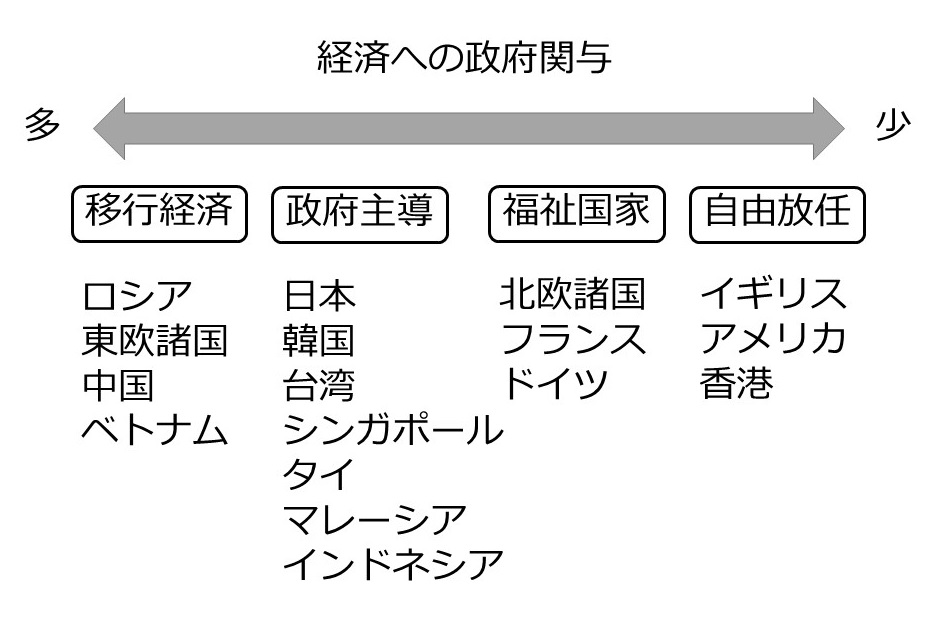
\includegraphics[width=960px]{poleco} \caption{経済への政府関与}\label{fig:poleco}
\end{figure}

\begin{figure}
\includegraphics[width=960px]{https://www.mof.go.jp/tax_policy/summary/condition/020} \caption{国民負担率(対国民所得比)の内訳の国際比較(日米英独仏瑞)}\label{fig:burden1}
\end{figure}

出所)\href{https://www.mof.go.jp/tax_policy/summary/condition/a04.htm}{財務省 ``負担率に関する資料''}

\begin{figure}
\includegraphics[width=960px]{https://www.mof.go.jp/tax_policy/summary/condition/238} \caption{国民負担率(対国民所得比)の国際比較(OECD加盟34カ国)}\label{fig:burden2}
\end{figure}

出所)図\ref{fig:burden1}と同じ

\begin{figure}
\includegraphics[width=960px]{https://www.mof.go.jp/tax_policy/summary/condition/019} \caption{国民負担率の推移}\label{fig:burden3}
\end{figure}

出所)図\ref{fig:burden1}と同じ

\begin{itemize}
\item
  資本主義・市場経済におけるその他の各国間の違いとして、企業の「所有と経営の分離」があります(図\ref{fig:separation})。

  \begin{itemize}
  \item
    中小企業では経営者が出資者であること、すわなちオーナー経営者がほとんどです。
  \item
    大企業になるにしたがって一人で出資金を出すことが難しくなったり、大きくなった企業を経営する能力に限界を感じるようになります。
  \item
    そのとき、他に出資者を求めたり、企業を経営能力の高い人に託すようになります。この状態を「所有と経営の分離」といいます。
  \end{itemize}
\item
  「所有と経営の分離」の状況によって、いくつかのグループに分けることができます。

  \begin{itemize}
  \item
    所有者と経営者が分離していて、経営者は主として所有者=株主(投資家)のために経営を行うのが、「株主資本主義」です。アメリカとイギリスがその代表的存在です。\protect\hyperlink{law}{法制度}はコモン・ローである国が多いです。
  \item
    所有者と経営者が分離していて、株主以外(従業員・地域)にも配慮した経営を行うのが、「ステークホルダー\footnote{将来役員になれるか(日本に比べ)比較的早い段階でわかるので、早期退社し起業する人が多いのがアジアの特徴です。韓国の現状については\href{https://toyokeizai.net/articles/-/473559}{菅野 (2021)}を参考にしてください。}資本主義」です。西欧諸国や日本が該当します。\protect\hyperlink{law}{法制度}はシビル・ローである国が多いです。
  \item
    所有者と経営者が分離してなく、大企業でも家族経営が多いのが「家族資本主義」です。多くの新興国が該当します。\protect\hyperlink{law}{法制度}の整備が十分でない国であることが多く、関係性による契約強制力が相対的に重要となっています。
  \item
    所有者と経営者が分離してなく、経営者の個人的縁故(コネ)がビジネスに影響するのが、「縁故資本主義」です。「家族資本主義」でもあることが多く、アジア、ラテンアメリカ、アラブの多くの国が該当します。
  \end{itemize}
\end{itemize}

\begin{figure}
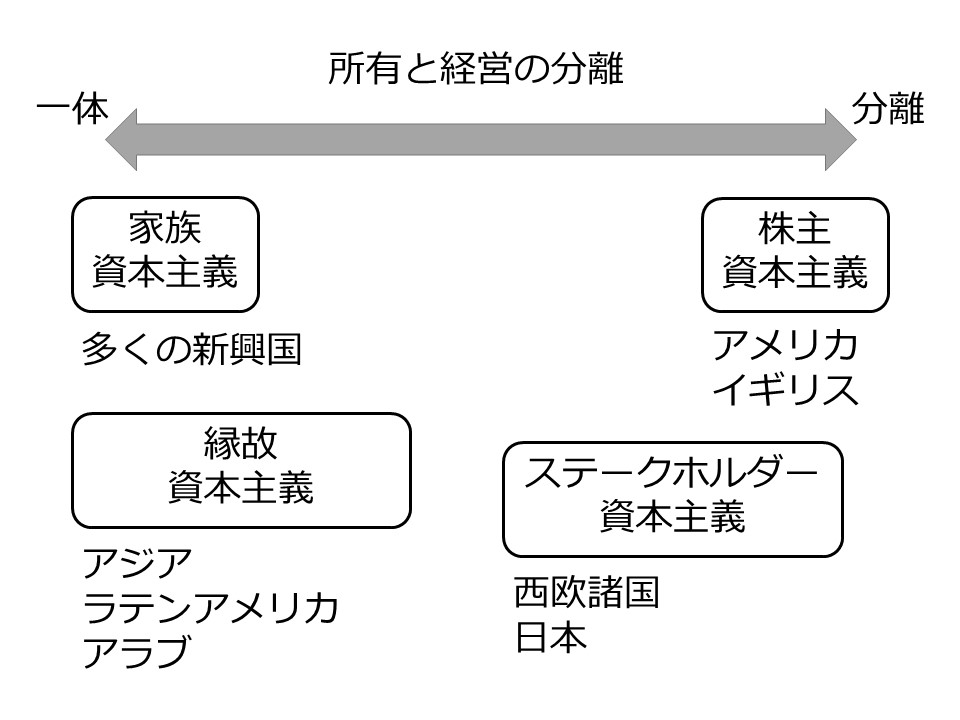
\includegraphics[width=960px]{separation} \caption{所有と経営の分離}\label{fig:separation}
\end{figure}

{\textbf{参考文献}}

\href{https://www3.nhk.or.jp/news/special/sakusakukeizai/articles/20200302.html}{NHK (2020a)「高すぎる? 国民負担率」}

\href{https://www.mof.go.jp/tax_policy/summary/condition/a04.htm}{財務省「負担率に関する資料」}

\hypertarget{usa}{%
\chapter{アメリカ企業の経営システム}\label{usa}}

\begin{itemize}
\item
  本章の構成は、以下のとおりです。

  \begin{itemize}
  \item
    \ref{us-external}では、アメリカ企業の経営システムの外部要因として、\ref{us-culture}文化、\ref{us-politics}政治システム・法制度、\ref{us-economy}経済システムを整理します。
  \item
    \ref{us-manager}では、アメリカ企業の経営者の特徴として、\ref{us-selection}選抜・移動、\ref{us-payment}報酬、\ref{us-education}教育を整理します。
  \item
    \ref{us-management}では、アメリカ企業の経営プロセスを\ref{us-plan}計画、\ref{us-organization}組織化、\ref{us-command}指揮・調整、\ref{us-control}統制を整理します。
  \end{itemize}
\end{itemize}

\hypertarget{us-external}{%
\section{アメリカの文化・政治・経済}\label{us-external}}

\begin{itemize}
\item
  本節では、アメリカ企業経営の外部要因として、アメリカの文化・政治・経済を確認します。

  \begin{itemize}
  \item
    まず、\protect\hyperlink{us-culture}{文化}を整理します。
  \item
    次に、\protect\hyperlink{us-politics}{政治システム・法制度}を整理します。
  \item
    最後に、\protect\hyperlink{us-economy}{経済システム}を整理します。
  \end{itemize}
\end{itemize}

\hypertarget{us-culture}{%
\subsection{文化}\label{us-culture}}

\hypertarget{ux6b74ux53f2}{%
\subsubsection{歴史}\label{ux6b74ux53f2}}

\begin{itemize}
\item
  1776年にイギリスからの独立を宣言し、アメリカ合衆国が建国されました\footnote{\href{https://plus.alc.co.jp/2018/01/meyer/}{他の国々との比較からあぶり出される日本文化の特徴やカルチャーマップの活かし方について}、著者がインタビューに答えています。}(イギリスが独立を認めたのは1783年のパリ条約)。国としての歴史は250年程度です。

  \begin{itemize}
  \item
    1492年にコロンブスが北アメリカ大陸を発見します。16世紀になると、イギリス、フランス、オランダ、スウェーデンなどが植民地を建設します。
  \item
    1620年にイギリスの清教徒(ピューリタン)\footnote{この違いは思考法だけでなく、\protect\hyperlink{law}{法体系}の違いにも影響を与えています。}がメイフラワー号でアメリカに移民します。
  \item
    その後、領土はイギリス、フランス、スペイン、メキシコなどから割譲あるいは併合し拡大し、1840年代には西海岸に到達しました。
  \end{itemize}
\end{itemize}

\begin{itemize}
\item
  人種構成は多様ですが、初期の移民の文化の影響が強いです。

  \begin{itemize}
  \item
    Weber(1905)\footnote{「平等主義的」でありながら「トップダウン式」のアメリカ、「階層主義的」でありながら「合意志向」のドイツ、日本は例外です。}は「プロテスタンティズムの倫理\footnote{山岸・ブリントン (2010)のいう\protect\hyperlink{labor}{セカンドチャンス}は、転職の文脈におけるこの状況を示していると解釈できます。}が、近代資本主義の成立について精神的側面から影響を及ぼした」と主張しました。
  \item
    清教徒(ピューリタン)など初期の移民が重視したのは個人の「自由」と神の前の「平等」であり、「フロンティア(開拓者)精神」です。ただし、当初の平等はキリスト教徒の白人男性が対象で、女性や黒人奴隷、先住民は含まれていませんでした(\href{https://yumenavi.info/lecture.aspx?GNKCD=g008685}{船津靖 ``「自由・平等・フロンティア精神」アメリカ人が最も大切にするもの''})。
  \item
    平等は時代を経て達成されていきますが、アメリカ社会における「プロテスタント系キリスト教徒のアングロサクソン系白人(WASP: White Anglo Saxon Protestant)」の影響力は依然として大きいです。

    \begin{itemize}
    \tightlist
    \item
      WASPでない大統領は、ケネディ大統領、オバマ大統領の2人だけです。\\
    \end{itemize}
  \item
    移民(アジア系、ヒスパニックなど)の増加と白人と非白人の出生率の差によって、2010年から2020年までの人口変化において、白人が減り、他の人種が増加しました(図\ref{fig:RACE}参照)。この傾向は継続し、人種構成において白人の割合は低下すると予想されています(表\ref{tab:USPOPULATION}参照)。

    \begin{itemize}
    \tightlist
    \item
      影響力の低下に不満を持つ白人が、トランプ(元)大統領の支持層となりました。
    \end{itemize}
  \end{itemize}
\end{itemize}

\begin{figure}
\includegraphics[width=960px]{https://assets.media-platform.com/bi/dist/images/2021/08/13/statics} \caption{アメリカの人種別人口増減}\label{fig:RACE}
\end{figure}

出所)\href{https://www.businessinsider.jp/post-240340}{BUSINESS INSIDER JAPAN ``史上初、アメリカで白人の人口が減った------ 2020年国勢調査''}

\begin{table}

\caption{\label{tab:USPOPULATION}アメリカの総人口における人種の割合}
\centering
\begin{tabular}[t]{c|c|c|c|c|c}
\hline
年 & 白人 & ヒスパニック & 黒人 & アジア & その他\\
\hline
2014年 & 62.2\% & 17.4\% & 12.4\% & 5.2\% & 2.9\%\\
\hline
2060年 & 43.6\% & 28.6\% & 13.0\% & 9.1\% & 5.7\%\\
\hline
\end{tabular}
\end{table}

出所)\href{https://www.nhk.or.jp/school/syakai/10min_tiri/kyouzai/001601.pdf}{NHK for School ``アメリカの総人口における人種の割合''}

\hypertarget{hofstedeux306eux6307ux6a19}{%
\subsubsection{Hofstedeの指標}\label{hofstedeux306eux6307ux6a19}}

\begin{itemize}
\item
  権力格差の指標は40で、低いほうに分類されます。

  \begin{itemize}
  \item
    上下関係は目的を果たすために必要な便宜的なものと捉えられます。社会的地位が高くても、人として平等と考えます。
  \item
    警察、軍隊などはっきりとした階級がある組織は例外ですが、民間企業ではファーストネームで呼び合うなど、役職で呼ぶことは少ないです。
  \item
    意思決定に関しては迅速さが求められる(短期志向:26)ため、民間企業でもトップダウン型です(\protect\hyperlink{meyer}{「Meyerのカルチャーマップ」の''決断''})。
  \end{itemize}
\item
  個人主義の指標は91で、世界的にみても高いです。

  \begin{itemize}
  \item
    個人の権利、自由、責任を強調し、ユニークさが尊重されます。
  \item
    労働者と企業は雇用契約書に職務(業務内容)を明記し、契約を結びます。

    \begin{itemize}
    \item
      労働者は企業に労働力という商品を売ると考えます。その価値を高めるために、経理、営業、マーケティング、広告といった専門能力を教育を通じ高めようとします。
    \item
      労働力は商品であるため、高く売れるところにすぐに移動する(転職が多い)傾向があります。
    \end{itemize}
  \end{itemize}
\item
  男性性の指標は62で、高いほうに分類されます。

  \begin{itemize}
  \item
    アメリカンドリームすなわち物質的成功を収めることが評価されます。
  \item
    社会進出する女性は多く、女性の企業経営者も増えていますが、一方で「ガラスの天井」\footnote{日本は例外です。}という見えない壁の存在も指摘されています(図\ref{fig:glassceiling})。
  \end{itemize}
\end{itemize}

\begin{figure}
\includegraphics[width=960px]{https://www.economist.com/img/b/1000/590/90/sites/default/files/20200307_WOC548} \caption{「ガラスの天井」指数の国際比較}\label{fig:glassceiling}
\end{figure}

出所)\href{https://www.economist.com/graphic-detail/2020/03/04/iceland-leads-the-way-to-womens-equality-in-the-workplace}{The Economist ``Iceland leads the way to women's equality in the workplace''}

\begin{itemize}
\item
  不確実性回避の指標は46で、低いほうに分類されます。

  \begin{itemize}
  \item
    開拓者として成功するためには誰よりも早く未開地に着くことが何より重要で、そのうえで大切なスピードを追求する過程でのある程度の失敗はやむを得ないとの考えが、今でも残っています。(Meyer. (2014, 日本語版 pp.186-187))
  \item
    起業し倒産することが「取り返しのつかない失敗」とはならないため、ベンチャー企業が多く誕生しています。
  \end{itemize}
\item
  長期志向の指標は26で、世界的にみても低いです。すなわち短期指向です。

  \begin{itemize}
  \item
    不確実性回避と同様に、開拓者精神から短期的利益を追求し、時間にも厳しいです。

    \begin{itemize}
    \item
      初対面の相手に親しく(柔らかく)接することが多く、笑顔を絶やさず、すぐにファーストネームで呼び始めたりします。(Meyer. (2014, 日本語版 p.217))
    \item
      ただし、このように友好的に振舞うことは素早くビジネスを始めるためのスキルであり、長く続く友情に発展するとは限りません。
    \end{itemize}
  \item
    長すぎる議論を嫌い、決断はいつでも修正できるとの考えのもと、不十分な情報に基づくものであっても\footnote{将来役員になれるか(日本に比べ)比較的早い段階でわかるので、早期退社し起業する人が多いのがアジアの特徴です。韓国の現状については\href{https://toyokeizai.net/articles/-/473559}{菅野 (2021)}を参考にしてください。}素早く決断を下すことを好みます。

    \begin{itemize}
    \tightlist
    \item
      感情的信頼を築くのに何時間もかけるのは時間の無駄遣いに感じる(Meyer. (2014, 日本語版 p.227))一方で、公私混同しないために仕事上の相手とは意図的に個人的な関係を築かないようにすることがプロフェッショナルであると考えます。(Meyer. (2014, 日本語版 pp.210-211))
    \end{itemize}
  \item
    山岸(1999, p.26)によると、質問紙調査で「アメリカ人は日本人よりもずっと、他者一般に対する信頼感が強い」という結果が出ています。
  \end{itemize}
\end{itemize}

\begin{itemize}
\item
  充足志向は68で、高いほうに分類されます。

  \begin{itemize}
  \item
    不確実性回避の指標が低いことや短期志向と関連しています。
  \item
    人前では喜びや楽観主義を表に出すと期待されています。
  \end{itemize}
\item
  アメリカは世界で最も低文脈な社会です。(Meyer. (2014, 日本語版 p.59))

  \begin{itemize}
  \item
    国民は世界各国からの移民で構成されています。移民はそれぞれ別々の歴史、別々の言葉、別々のバックグラウンドを持っています。

    \begin{itemize}
    \tightlist
    \item
      建国以来の歴史も短いため、共有する文脈が少なくなります。
    \end{itemize}
  \item
    メッセージを伝える際は曖昧さや誤解が生じる余地をなくして、できるだけはっきりと明快に伝えることが、コミュニケーションの基本になります。
  \end{itemize}
\end{itemize}

\hypertarget{us-politics}{%
\subsection{政治システム・法制度}\label{us-politics}}

\begin{itemize}
\item
  アメリカは民主主義国家であり、三権分立が確立しているため、政治は安定しています。

  \begin{itemize}
  \tightlist
  \item
    ジャーナリズムが独立しており、政治家や企業の不正は厳しく追及されます。
  \end{itemize}
\item
  アメリカではさまざまな価値観が認められますが、政党としては「保守」系の共和党と「リベラル」系の民主党の二大政党に概ね集約されます(図\ref{fig:USPARTY})。

  \begin{itemize}
  \tightlist
  \item
    二大政党の間で政権交代が繰り返されています。大統領は1期4年で、再選されると2期8年まで可能です。
  \end{itemize}
\item
  大統領選においては各党の候補者選びから1年をかけて討論を重ねるため、将来実施されるであろう政策も予想が立ち(またある程度の政策の継続性も期待でき)ます。

  \begin{itemize}
  \tightlist
  \item
    政権交代があっても「政策の予測可能性」が高いことから、企業は長期(5〜10年)の経営・設備投資計画が立てやすくなります。
  \end{itemize}
\end{itemize}

\begin{figure}
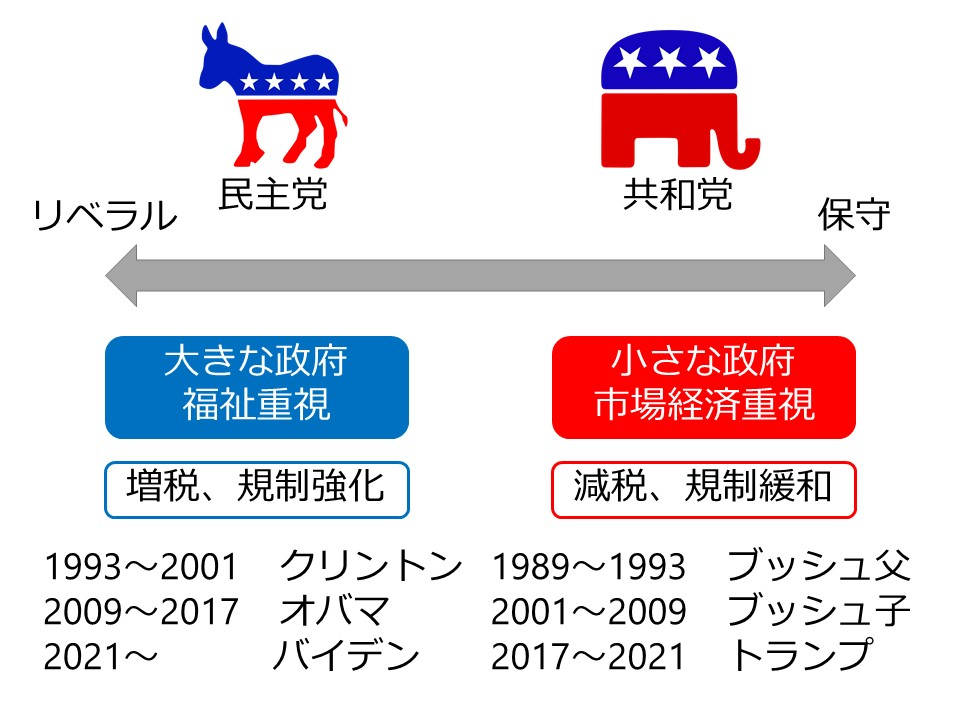
\includegraphics[width=960px]{usparty} \caption{アメリカの二大政党}\label{fig:USPARTY}
\end{figure}

\begin{itemize}
\item
  多民族国家で低文脈社会であることから、法律や契約書は条文が詳細に記載されます\footnote{学歴重視社会・競争社会は、若年層の失業問題などの社会問題を引き起こしています。中国の現状については\href{https://diamond.jp/articles/-/277433}{王 (2021)}、韓国の現状については\href{https://hbol.jp/pc/189601/}{和場ほか (2019a)}、\href{https://hbol.jp/pc/189810/}{和場ほか (2019b)}を参考にしてください。}。

  \begin{itemize}
  \tightlist
  \item
    契約の強制は司法制度が重要になります(\ref{us-management}\protect\hyperlink{law}{法制度} )。
  \end{itemize}
\end{itemize}

\begin{itemize}
\item
  自由競争を重んじるため、経済に対する政府関与の度合いは他国に比べ低いです。

  \begin{itemize}
  \tightlist
  \item
    自由競争を阻害する独占や寡占を禁止する独占禁止法(反トラスト法)により、スタンダード・オイルやAT\&Tなど巨大企業が分割されたこともあります\footnote{日本経済新聞朝刊 2021年11月21日「女性・外国人取締役、主要企業の半数でゼロ」}。
  \end{itemize}
\end{itemize}

\hypertarget{us-economy}{%
\subsection{経済システム}\label{us-economy}}

\begin{itemize}
\item
  アメリカ経済の特徴は、経済的自由の高さです。

  \begin{itemize}
  \item
    経済規模は世界一であり、数多くの外国企業が参入してきます。
  \item
    起業、買収・合併(M\&A)、倒産が頻繁に起こるなど、市場競争が厳しいです。

    \begin{itemize}
    \tightlist
    \item
      起業が多いのは、不確実性回避の指標が低いことが背景にあります。
    \end{itemize}
  \end{itemize}
\item
  高い経済的自由の背景として、柔軟な労働市場の存在が挙げられます。

  \begin{itemize}
  \item
    不景気で労働力に余剰が生まれたとき、容易にレイオフ(一時解雇)\footnote{\href{https://www.nikkei.com/article/DGXZQOCC1454K0U1A510C2000000/}{日本経済新聞電子版 2021年5月15日「女性の管理職比率とは 米欧先行、日本は10\%台」}}を行うことができます。

    \begin{itemize}
    \tightlist
    \item
      日本ではレイオフではなく、雇用を確保した上で時短が行われることが多いです(図\ref{fig:layoff})。
    \end{itemize}
  \item
    不景気のときに容易にレイオフできることから、企業は好景気で人手不足になったときは採用を積極的に行います。

    \begin{itemize}
    \tightlist
    \item
      これを労働市場の流動性が高いといいます。
    \end{itemize}
  \item
    レイオフされた労働者は再雇用を待たなくても、(レイオフされた企業よりも業績がいい=賃金水準の高い)他社に比較的容易に再就職できます。
  \item
    アメリカの労働者は専門性を持っていて、職種ごとに採用されるため、転職先の仕事を学びなおす必要がありません。

    \begin{itemize}
    \tightlist
    \item
      労働市場の流動性が高いことは、労働者にとって決してマイナスとはいえないことになります。
    \end{itemize}
  \item
    経済全体から見ても、不況業種から好況業種へ労働力が移動するというプラスの効果があります。
  \end{itemize}
\end{itemize}

\textbackslash begin\{figure\}
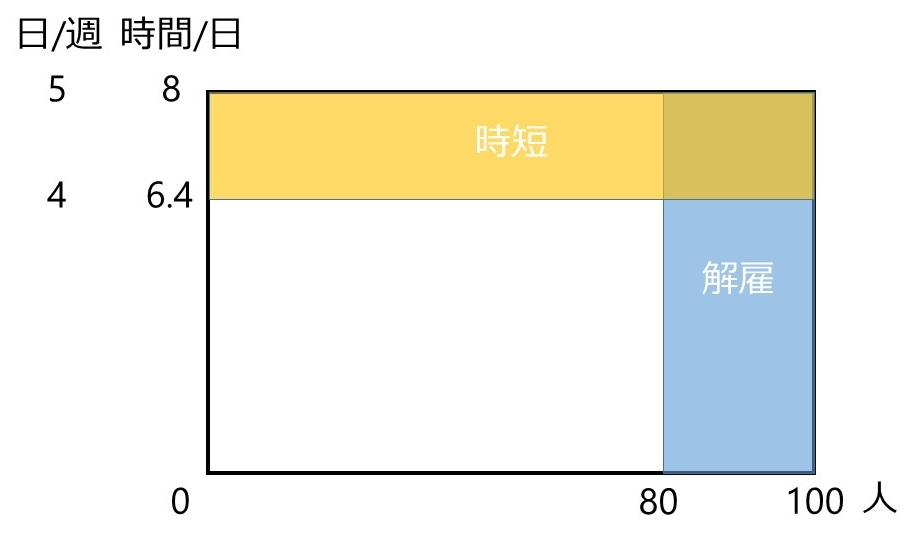
\includegraphics[width=960px]{layoff} \textbackslash caption\{労働時間20\%削減の方法\}\label{fig:layoff}
\textbackslash end\{figure\}

\begin{itemize}
\item
  高い経済的自由の背景として、発達した金融市場の存在が挙げられます。

  \begin{itemize}
  \item
    証券市場が発達していて、他国と比較して企業は証券市場から多く資金を調達します。
  \item
    起業する場合でも、ベンチャーキャピタル\footnote{CEOの学歴として、「大卒」は国際的には低学歴といえます。}からの資金調達が可能です。

    \begin{itemize}
    \tightlist
    \item
      借入(負債)でなく、株式(資本)での資金調達が多いため、倒産したときのリスクは起業家ではなく、投資家が負担することになります。
    \end{itemize}
  \item
    金融制度の面からも、倒産からの再チャレンジが容易となっています。

    \begin{itemize}
    \tightlist
    \item
      不確実性回避の指標が低いのも、文化的要因だけでなく社会制度にも起因するものと考えられます。
    \end{itemize}
  \end{itemize}
\end{itemize}

\begin{itemize}
\item
  経済への政府関与は低いです。経済規模に比べ政府支出は少なく、国営企業も少ないです。

  \begin{itemize}
  \item
    年金や健康保険といった社会保障は、他国に比べ民間部門が担う部分が大きいです。

    \begin{itemize}
    \item
      アメリカでは一部を除き、基本的に健康保険(医療保険)は個人で民間保険に加入します。
    \item
      アメリカの医療費は高いことで有名で、盲腸の手術で150~440万円するとされます(\href{https://www.med.or.jp/people/info/kaifo/compare/\#:~:text=\%E5\%9C\%A8\%E3\%83\%8B\%E3\%83\%A5\%E3\%83\%BC\%E3\%83\%A8\%E3\%83\%BC\%E3\%82\%AF\%E7\%B7\%8F\%E9\%A0\%98\%E4\%BA\%8B\%E9\%A4\%A8\%E3\%81\%AE,\%E3\%82\%92\%E6\%B1\%BA\%E5\%AE\%9A\%E3\%81\%97\%E3\%81\%A6\%E3\%81\%84\%E3\%81\%BE\%E3\%81\%99\%EF\%BC\%89\%E3\%80\%82}{日本医師会 ``アメリカは医療格差社会''})。
    \item
      健康保険は給与の一部として支給されることも多い一方、失業すると収入だけでなく健康保険も失うことになるので、影響が大きいです。
    \end{itemize}
  \end{itemize}
\item
  アメリカ社会では、機会の平等は高く求められます。

  \begin{itemize}
  \tightlist
  \item
    人種や性別、民族などによる社会的差別を改善し、雇用や教育などにおいて採られる優遇措置をアファーマティブ・アクション(積極的格差是正措置)といいます。
  \end{itemize}
\item
  その一方で、家計の所得・資産の不平等は大きいです(結果の不平等)。

  \begin{itemize}
  \item
    上位1\%の人たちの所得は1981年に全体の8.2\%でしたが、2012年には倍以上の20\%に高まっています(図\ref{fig:inequality})。その一方で、所得が最も少ない10\%の層の人たちの収入は、2000年から2008年の間に実質で10\%減少しました(\href{https://www.nli-research.co.jp/report/detail/id=42347?site=nli}{櫨 (2015)})。
  \item
    アファーマティブ・アクションによっても、人種間の所得・資産格差は存在し続けています。2019年の典型的な非ヒスパニック系白人世帯の純資産は、非ヒスパニック系黒人世帯の約8倍でした(\href{https://www.cnn.co.jp/business/35172251.html}{CNN.co.jp (2021)})。
  \end{itemize}
\end{itemize}

\textbackslash begin\{figure\}
\includegraphics[width=960px]{https://www.nli-research.co.jp/files/user/report/report/2015/04/image/repo1504-1.jpg?v=1448125638} \textbackslash caption\{上位1\%の人たちの所得シェア\}\label{fig:inequality}
\textbackslash end\{figure\}

出所)\href{https://www.nli-research.co.jp/report/detail/id=42347?site=nli}{櫨 (2015)}

{\textbf{参考文献}}

\href{https://www.cnn.co.jp/business/35172251.html}{CNN.co.jp (2021)「4つのグラフから見る 米国の黒人と白人の格差」}

Meyer, E. (2014). The Culture Map: Breaking Through the Invisible Boundaries of Global Business. PublicAffairs.(日本語版 樋口武志(訳)・田岡恵(監訳)(2015)『異文化理解力』英治出版.)

\href{https://www3.nhk.or.jp/news/special/sakusakukeizai/articles/20201023.html}{NHK (2020b)「グーグルに何が起きているの?」}

Weber, Max (1905). Die protestantische Ethik und der Geist des Kapitalismus. (日本語版 大塚久雄(訳)(1989)『プロテスタンティズムの倫理と資本主義の精神』岩波文庫.)

\href{https://www.nli-research.co.jp/files/topics/42347_ext_18_0.pdf?site=nli}{櫨浩一 (2015)「巻き起こる格差議論-ピケティ「21世紀の資本」の意味」基礎研REPORT 2015年4月号}

山岸俊男 (1999)『安心社会から信頼社会へ』中公新書1479.

\hypertarget{us-manager}{%
\section{アメリカ企業の経営者}\label{us-manager}}

\begin{itemize}
\item
  本節では、アメリカ企業の経営者に関連する項目を整理します。

  \begin{itemize}
  \item
    まず、アメリカ企業の経営者のキャリア形成のプロセス、\protect\hyperlink{us-selection}{選抜・移動}を整理します。
  \item
    次に、アメリカ企業の経営者の\protect\hyperlink{us-payment}{報酬}について、概要を整理します。
  \item
    最後に、アメリカ企業の経営者の教育的背景(学歴)や、経営学の\protect\hyperlink{us-education}{教育}の位置付けについて整理します。
  \end{itemize}
\end{itemize}

\hypertarget{us-selection}{%
\subsection{選抜・移動}\label{us-selection}}

\begin{itemize}
\item
  \href{https://www.strategyand.pwc.com/jp/ja/publications/2018_ceo-data-media-release-jp.pdf}{Strategy\& (2019)}が行った、世界の上場企業における時価総額の上位2,500社を対象にした調査によると、アメリカ企業の経営者(最高経営責任者CEO:Chief Executive Officer)の平均像は、以下の通りです。 \protect\hyperlink{japan-selection}{日本} \protect\hyperlink{asia-selection}{アジア}

  \begin{itemize}
  \item
    2018年に就任したCEOの年齢の中央値は54才です。
  \item
    内部昇格したCEOが79\%で、外部招聘のCEOが21\%でした。

    \begin{itemize}
    \item
      新任CEOの94\%が他企業での職務経験があります。
    \item
      ヘッドハンティングが盛んで、プロ経営者(A社社長退任→B社社長就任)もいます。

      \begin{itemize}
      \tightlist
      \item
        新任CEOの26\%が株式公開会社でのCEO経験を有しています。
      \end{itemize}
    \end{itemize}
  \item
    海外での勤務経験を有するCEOは33\%でした。
     

    \begin{itemize}
    \item
      世界平均レベルですが、西欧諸国(63\%)に比べると低いです。
    \item
      Edfelt (2010, pp.50-52)によると、アメリカ企業は以下の特徴があります。

      \begin{itemize}
      \item
        海外に居住・勤務経験のある経営者は1/3
      \item
        「経営者に国際経験は重要?」との問いには、Yesは15\%、Noは54\%
      \item
        「国際ビジネスに外国語は必要?」との問いには、同意と多少同意の合計が34\%
      \end{itemize}
    \end{itemize}
  \item
    新任CEOの85\%がアメリカ国籍でした。
  \item
    新任CEOの女性比率は1.1\%でした。
     

    \begin{itemize}
    \item
      \href{https://forbesjapan.com/articles/detail/990}{Forbes JAPAN (2014)}によると、アメリカの全企業の23\%の780万社が女性が経営する企業であり、特に、ヘルスケア・教育サービス分野では、61\%の企業が女性CEOです。
    \item
      この20年間、女性の起業率は男性の2倍であることから、「ガラスの天井」を感じた女性が多く起業したと考えられます。
    \end{itemize}
  \item
    新任CEOの53\%がMBA(経営学修士)保有者です。

    \begin{itemize}
    \tightlist
    \item
      世界平均(33\%)を大きく上回ります。
    \end{itemize}
  \item
    民間と政府で相互に転職することがあり、「回転ドア」と呼ばれます。民間経営者が政府高官になることもあります。
  \end{itemize}
\item
  移動の多さは、個人主義の高さや不確実性回避の低さから解釈できます。
\end{itemize}

\hypertarget{us-payment}{%
\subsection{報酬}\label{us-payment}}

\begin{itemize}
\tightlist
\item
  \href{https://www.wtwco.com/ja-JP/News/2022/08/report-fy2021-comparison-of-compensation-for-ceos-and-ned-between-japan-the-united-states-and-europe}{ウイリス・タワーズワトソン (2022)} によると、アメリカ企業CEOの報酬(2021年度)の中央値は16.0億円でした(図\ref{fig:g5ceopay})。
\end{itemize}

\begin{figure}
\includegraphics[width=960px]{https://media.wtwco.com/-/media/WTW/News/2022/08/report-fy2021-comparison-of-compensation-01.png?modified=20220817061527&imgeng=meta_true} \caption{CEO報酬比較(2021年度)}\label{fig:g5ceopay}
\end{figure}

出所)\href{https://www.wtwco.com/ja-JP/News/2022/08/report-fy2021-comparison-of-compensation-for-ceos-and-ned-between-japan-the-united-states-and-europe}{ウイリス・タワーズワトソン (2022)}

\begin{itemize}
\tightlist
\item
  ダウ平均の構成企業でみると、経営トップの年間報酬で最高額だったのはナイキの5349万ドル(58.3億円)です(表\ref{tab:uspay})。
\end{itemize}

\begin{table}

\caption{\label{tab:uspay}ダウ平均構成30社の社長の年収(1~5位)}
\centering
\begin{tabular}[t]{r|l|l|l|l|l|l|l}
\hline
順位 & 社長.CEO.名 & 社名 & 年収 & 前期比増減率 & 株式報酬の割合 & 従業員の年収に対する倍率 & 株価騰落率\\
\hline
1 & ジョン・ドナホー & ナイキ & 58.3億円 & ー & 83\% & 1935倍 & 28\%\\
\hline
2 & サティア・ナデラ & マイクロソフト & 48.3億円 & 3\% & 69\% & 257倍 & 52\%\\
\hline
3 & ジェームズ・ダイモン & JPモルガン・チェース & 34.5億円 & 0\% & 79\% & 395倍 & -10\%\\
\hline
4 & アレックス・ゴースキー & ジョンソン・エンド・ジョンソン & 32.2億円 & 17\% & 61\% & 365倍 & 7\%\\
\hline
5 & マイケル・ワース & シェブロン & 31.6億円 & -12\% & 52\% & 184倍 & -29\%\\
\hline
\end{tabular}
\end{table}

注)1ドル=109円で換算\\
出所)日経ヴェリタス(日経電子版)\footnote{経団連については、\href{https://gakumado.mynavi.jp/style/articles/46464}{マイナビ (2020) ``「経団連」とは? 今さら聞けないその言葉の意味・役割・取り組みを解説''}などを参考にしてください。}

\begin{itemize}
\item
  企業の経営トップの報酬が従業員の賃金の何倍かを示す数値を\textbf{ペイレシオ(pay ratio)}といいます。

  \begin{itemize}
  \item
    日本経済新聞\footnote{日本経済新聞朝刊 2018年6月18日「変わる経団連、変われぬ経団連」}によると、ペイレシオが高い企業(2018年の公表当時)3社はマクドナルド3101倍、ウォルマート1188倍、ジョンソン・エンド・ジョンソン452倍となっています。
  \item
    \href{https://www.dir.co.jp/report/column/20170921_012304.html}{鈴木 (2017)}によれば、アメリカ企業のペイレシオは「1965年には平均20倍であったものが、1989年に59倍、2000年に376倍になったのち、2016年では271倍」に拡大しています。
  \end{itemize}
\end{itemize}

\begin{itemize}
\tightlist
\item
  アメリカ企業の経営者の報酬が高額である背景には、その報酬多くが業績連動報酬\footnote{日経産業新聞 2018年6月22日「経団連 この恐るべき同質集団」}であるためです。
\end{itemize}

\begin{itemize}
\item
  業績連動報酬のなかでは、「あらかじめ決められた価格(図\ref{fig:stockoption}では1円)で株式を購入できる」ストック・オプションが代表的存在です。

  \begin{itemize}
  \tightlist
  \item
    ストック・オプションは、経営者にとって「業績向上⇒企業価値の向上⇒株価の上昇⇒売却益増」といった好循環に対するインセンティブとして有効な制度となり得ます。
  \end{itemize}
\end{itemize}

\begin{figure}
\includegraphics[width=960px]{https://www.dir.co.jp/business/consulting/compensation/gdp1m8000003nqos-img/img-introduction-01} \caption{ストック・オプションのスキームイメージ}\label{fig:stockoption}
\end{figure}

出所)\href{https://www.dir.co.jp/business/consulting/compensation/stock-option.html}{大和総研}

\hypertarget{us-education}{%
\subsection{教育}\label{us-education}}

\begin{itemize}
\item
  アメリカ企業のCEOは高学歴といえます\footnote{日本経済新聞朝刊 2020年7月19日「社長の報酬、日米で格差12倍に 19年度 業績連動部分少なく」によると、自社の現物株を報酬として付与する企業が、2020年6月末時点で800社超と過去1年間で5割増えまし
    た。日本では報酬全体の57\%が固定給ですが、アメリカではわずか9\%です。}。

  \begin{itemize}
  \item
    Edfelt (2010, pp.42-43)によると、アメリカ企業CEOの学歴は以下の特徴があります。

    \begin{itemize}
    \item
      大企業CEOの98\%が大卒で、専攻の内訳は工学21\%、経済学15\%、経営学13\%です。
    \item
      修士以上の学位をもつアメリカ人は、25才以上人口の10\%に過ぎませんが、大企業CEOの67\%が修士以上の学位を保有しています。
    \item
      大企業CEOの保有する修士以上の学位の内訳はMBA40\%、法学10\%となりますが、MBA以外の学位のうち21\%はPh.D.(博士号)です。
    \end{itemize}
  \item
    \href{https://warp.da.ndl.go.jp/info:ndljp/pid/11486206/db.jil.go.jp/db/seika/zenbun/E2000014381_ZEN.htm}{日本労働研究機構 (1998)}の調査によると、アメリカ企業の人事・営業・経理部課長は32-40\%がMBAを保有し、Ph.D.(博士号)保有者もいます(図\ref{fig:uscareer})。
  \end{itemize}
\end{itemize}

\begin{figure}
\includegraphics[width=960px]{https://warp.da.ndl.go.jp/info:ndljp/pid/11486206/db.jil.go.jp/db/seika/zenbun/IMAGE/E2000014381-ZU127} \caption{アメリカ企業部課長職の学歴}\label{fig:uscareer}
\end{figure}

出所)\href{https://warp.da.ndl.go.jp/info:ndljp/pid/11486206/db.jil.go.jp/db/seika/zenbun/E2000014381_ZEN.htm}{日本労働研究機構 (1998)}

\begin{itemize}
\item
  アメリカにおいて、経営学は学問として広く認知されています。

  \begin{itemize}
  \tightlist
  \item
    全米の大学学部の22\%、大学院修士課程の25\%に経営学専攻があります(Edfelt (2010, p.43))。
  \end{itemize}
\item
  アメリカ企業において、内部昇進・転職に伴う昇進に関わらず、昇進には職位に見合った能力が求められますが、その証明として学位が多く利用されます。

  \begin{itemize}
  \item
    アメリカに限らず欧米では、「仕事」の内容、範囲、責任、権限などを「職務記述書」ないし「権限規程」などの様式に、誰がみてもまぎれのないように明確に決めています(濱口 (2013, p.30))。
  \item
    採用は図\ref{fig:uspost}のように「必要なときに、必要な資格、能力、経験のある人を、必要なだけ」採用する欠員補充が原則となります(濱口 (2013, p.40))。
  \item
    一つ一つの職業について、その職業を遂行する知識、経験、能力を兼ね備えた一人前の労働力に対する職種別の賃金が決まっています(濱口 (2013, p.85))。
  \end{itemize}
\end{itemize}

\begin{figure}
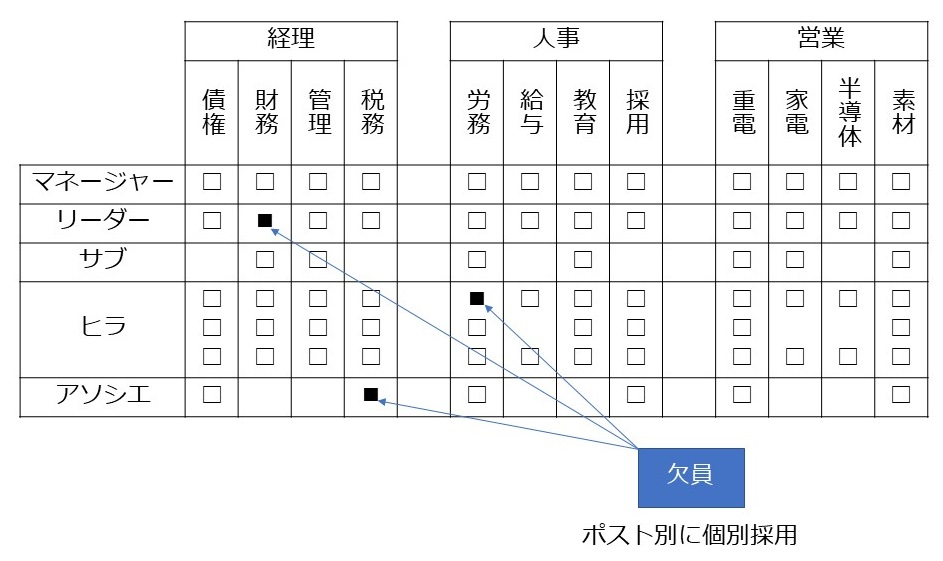
\includegraphics[width=960px]{uspost} \caption{欧米の採用}\label{fig:uspost}
\end{figure}

出所)海老原 (2016)

{\textbf{参考文献}}

Edfelt, Ralph B. (2010). Global Comparative Management. SAGE.

\href{https://forbesjapan.com/articles/detail/990}{Forbes JAPAN (2014)「アメリカ出世事情・女性CEOが誕生する理由」}

Meyer, E. (2014). The Culture Map: Breaking Through the Invisible Boundaries of Global Business. PublicAffairs.(日本語版 樋口武志(訳)・田岡恵(監訳)(2015)『異文化理解力』英治出版.)

\href{https://www.strategyand.pwc.com/jp/ja/publications/2018_ceo-data-media-release-jp.pdf}{Strategy\& (2019)「2018年 CEO 承継調査」}

\href{https://www.willistowerswatson.com/ja-JP/News/2021/07/report-fy2020-comparison-of-compensation-for-ceos-and-ned-between-japan-the-united-states-and-europe}{ウイリス・タワーズワトソン (2021)「ウイリス・タワーズワトソン、 『日米欧CEOおよび社外取締役報酬比較』 2021年調査結果を発表」}

海老原嗣生 (2016)『お祈りメール来た、日本死ね』文春新書1105.

\href{https://www.recme.jp/careerhigh/entry/usaceo}{キャリハイ転職「「元軍人から高校からはじめたバイトまで」P\&G、Apple等、米国時価総額トップ15人のCEOの経歴を調べた」}

\href{https://www.dir.co.jp/report/column/20170921_012304.html}{鈴木裕 (2017)「社長の報酬は社員の何倍?---米英で分かれたペイレシオ開示政策---」大和総研}

\href{https://www.dir.co.jp/business/consulting/compensation/stock-option.html}{大和総研 ``ストック・オプション導入コンサルティング''}

\href{https://warp.da.ndl.go.jp/info:ndljp/pid/11486206/db.jil.go.jp/db/seika/zenbun/E2000014381_ZEN.htm}{日本労働研究機構 (1998)「国際比較:大卒ホワイトカラーの人材開発・雇用システム -日、米、独の大企業」}

濱口桂一郎 (2013)『若者と労働』中公新書ラクレ465.

\hypertarget{us-management}{%
\section{アメリカ企業のマネジメント}\label{us-management}}

\begin{itemize}
\item
  本節では、アメリカ企業のマネジメントに関連する項目を整理します。

  \begin{itemize}
  \item
    まず、アメリカ企業の\protect\hyperlink{us-plan}{計画}を整理します。
  \item
    次に、アメリカ企業の\protect\hyperlink{us-organization}{組織化}について、概要を整理します。
  \item
    次に、アメリカ企業の\protect\hyperlink{us-command}{指揮・調整}について、概要を整理します。
  \item
    最後に、アメリカ企業の\protect\hyperlink{us-control}{統制}について、概要を整理します。
  \end{itemize}
\end{itemize}

\hypertarget{us-plan}{%
\subsection{計画}\label{us-plan}}

\begin{itemize}
\item
  Fayolの「計画(planning)」は、目的達成のための活動計画(年次予算や中期経営計画など)を策定することです。\protect\hyperlink{fayol}{Fayolの経営管理プロセス}

  \begin{itemize}
  \item
    短期(月次・年間)の計画は「予算」といわれます。生産数量また生産に必要な原材料の数量や販売価格を決め、売上と費用から利益の見込み・目標を立てます。
  \item
    生産販売計画が決まると、それを実現するための投資計画を立てる必要があります。通常、数年間の投資回収期間を想定します。
  \item
    予算とは別に、中期(3-5年)、長期(10年)など、経営者の在任期間あるいはそれ以上の計画も立てることがあります。
  \end{itemize}
\item
  アメリカ企業は他国よりも戦略的な長期計画を策定を好む傾向があります(Edfelt (2010, p.52))。

  -アメリカ企業は他国よりも専門家(経営コンサルタント)を雇い、計画を立てることが多いです。

  \begin{itemize}
  \item
    コンサルティングは、19世紀末の技術者による時間動作(能率)研究が発祥です。計画を立て効率的に業務を遂行するのは、Taylorの科学的管理法にまで遡れます。
  \item
    計画の範囲は時代を追うごとに、範囲を広げ高度になります。

    \begin{itemize}
    \item
      1950-60年代は生産の場所(工場立地)、時間、規模、範囲という「生産計画」が中心でした。
    \item
      1960-70年代になると、政治・経済・技術・文化他の評価、企業内部の強みと限界といったSWOT分析を踏まえた戦略が計画に組み込まれます。
    \item
      1980年代以降は、戦略性をもって計画を立てることは、経営そのものとなります。
    \end{itemize}
  \item
    計画の範囲が広がるのに応じて、コンサルティングにも変化が生じました。

    \begin{itemize}
    \item
      1970年代までには、会計事務所は従来から行ってきた税務・監査業務のほかに、経営コンサルティング(マネジメント助言)を提供するようになりました。
    \item
      1980年代には、コンサルティング業はさらに発展し、財務会計や税務に加え、生産システム、情報システムをも含む助言を行うようになりました。
    \end{itemize}
  \end{itemize}
\item
  経営学が学問として認知され信頼されていること、また不確実性回避の傾向が低いことから、新しい経営手法を積極的に導入する傾向があります。
\end{itemize}

\hypertarget{us-organization}{%
\subsection{組織化}\label{us-organization}}

\begin{itemize}
\item
  Fayolの「組織化(organizing)」は、製造や営業といった事業活動が効率良く実行されるような組織構造(人と仕事の配置)を構築することです。\protect\hyperlink{fayol}{Fayolの経営管理プロセス}

  \begin{itemize}
  \tightlist
  \item
    企業にとって望ましい組織は、環境(規模、戦略など)によって異なります。
  \end{itemize}
\item
  企業規模が小さく、製品数が少ない企業は機能別組織が適しています(図\ref{fig:org1}参照)。

  \begin{itemize}
  \item
    機能別組織のメリットは、専門性を高めやすいことです。
  \item
    経営者に権限が集中するシンプルな階層構造のため、統制を図りやすいです。
  \item
    機能別組織のデメリットは、組織が大きくなると経営者の負担が大きくなることです。
  \item
    部門管理者が専門化することで全社的なマネジメント力がある人材が育ちにくい面もあります。
  \end{itemize}
\end{itemize}

\begin{figure}
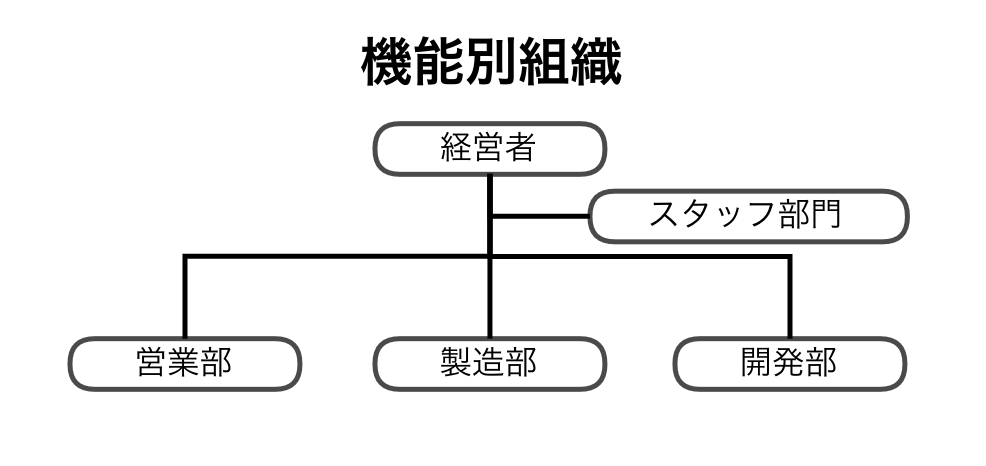
\includegraphics[width=960px]{org1} \caption{機能別組織}\label{fig:org1}
\end{figure}

出所)\href{https://life-is-yuyu.com/consultant/business-management/function-divisional/}{ゆうゆうぶろぐ (2020)}

\begin{itemize}
\item
  企業規模が大きく、大規模で製品数が多いと事業部制組織が適しています(図\ref{fig:org2}参照)。

  \begin{itemize}
  \item
    事業部別組織のメリットは、意思決定が速くなることです。
  \item
    経営者が業務的管理から解放され、戦略的意思決定に多くの時間を使えるようになります。
  \item
    事業部別組織のデメリットは、各事業部の機能が重複することでコストがかさむことです。
  \item
    各事業部がそれぞれの利益の達成にこだわり、全社的には最適な意思決定ができない恐れがあります。
  \end{itemize}
\end{itemize}

\begin{figure}
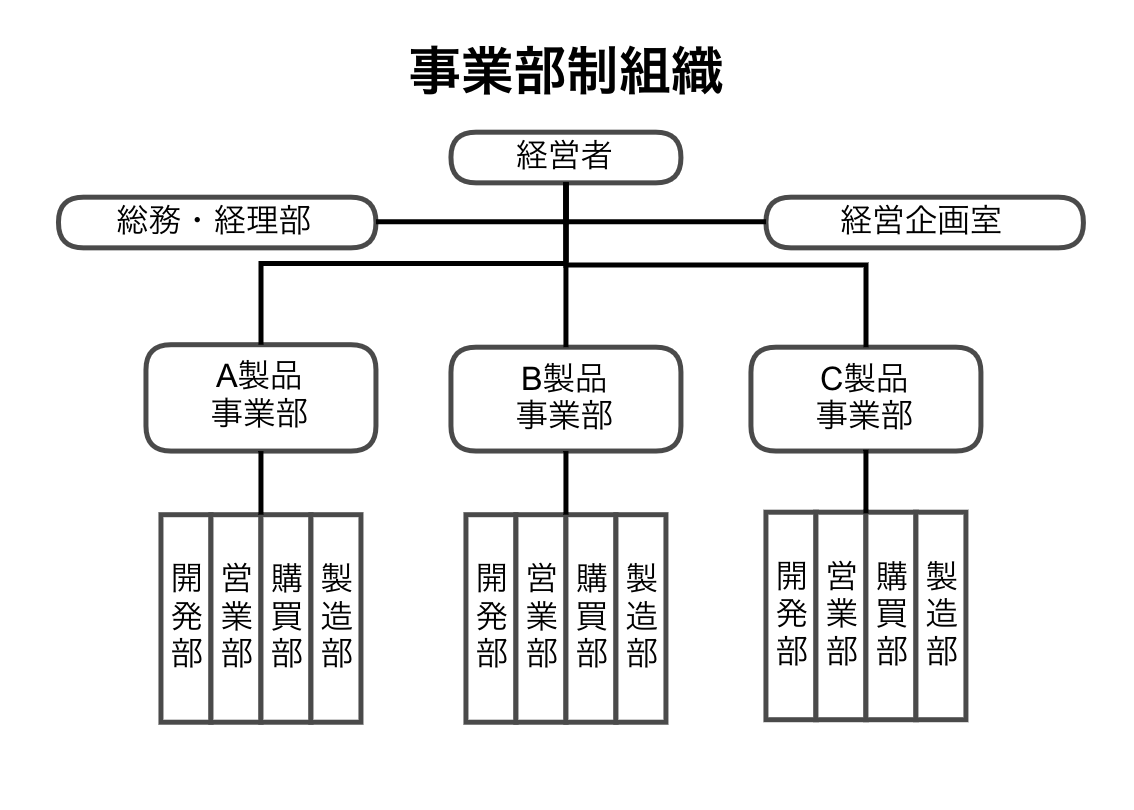
\includegraphics[width=960px]{org2} \caption{事業部制組織}\label{fig:org2}
\end{figure}

出所)図\ref{fig:org1}と同じ

\begin{itemize}
\item
  アメリカで事業部制組織が採用されたのは、1920年代のデュポンやGMとされています。

  \begin{itemize}
  \tightlist
  \item
    1914年に第一次世界大戦が始まり欧州が戦場となったことで、戦後(1920年代以降)経済の中心がヨーロッパからアメリカへ移動しました。
  \end{itemize}
\item
  急速な事業拡大に対応するには迅速な意思決定が必要であり、そのために分権化(権限移譲)が必要だったため、事業部制組織が採用されるようになりました。
   

  \begin{itemize}
  \tightlist
  \item
    アメリカは権力格差が低いため、権限委譲を進めやすく、部下もそれを受け入れやすかったといえます。
  \end{itemize}
\item
  組織変化(改編)は企業内だけでなく、企業間でも行われます。

  \begin{itemize}
  \item
    買収(Merger)、合併(Acquisition)を合わせ、M\&Aといいます(図\ref{fig:ma}参照)。

    \begin{itemize}
    \tightlist
    \item
      買収側にとってM\&Aの大きな目的は時間を買うことができることです。売却側にとっては、投資回収までの時間を大幅に短縮し、資本を得ることが可能になります。どちらも短期志向であるといえます。
    \end{itemize}
  \item
    投資銀行という金融機関が、企業にM\&Aを提案し諸手続きをアドバイスする役目を果たします。
  \item
    アメリカでは(被合併・買収企業が反対する)敵対的買収もしばしば行われます。
  \item
    M\&Aによって活発に業界が再編されるのも、不確実性回避が低く、変化を厭わないためといえます。

    \begin{itemize}
    \tightlist
    \item
      1957年のS\&P500社で1997年に残っているのは74社(14.8\%)のみです。(Edfelt (2010, p.63))
    \end{itemize}
  \end{itemize}
\end{itemize}

\begin{figure}
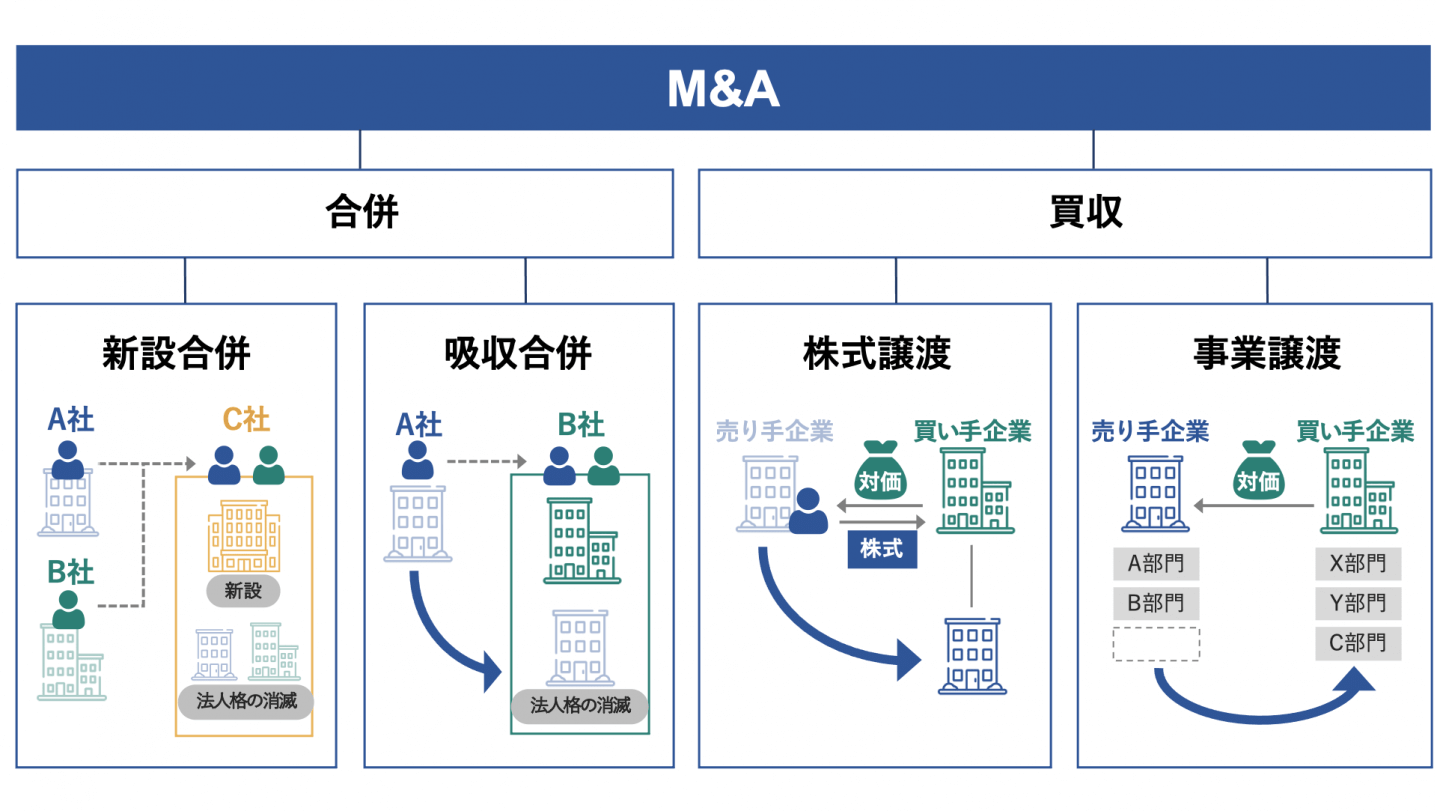
\includegraphics[width=960px]{ma} \caption{M&Aの種類}\label{fig:ma}
\end{figure}

出所)\href{https://br-succeed.jp/content/knowledge/post-1598}{BIZREACH SUCCEED (2021)}

\hypertarget{us-command}{%
\subsection{指揮・調整}\label{us-command}}

\begin{itemize}
\item
  Fayolの「指揮(commanding)」は、各部門の役割と責任、そして目標数値を設定し達成に向けて、指示を与え、働かせることです。「調整(coordinating)」は、目標が達成できるように、部分最適になりがちな各部門・個人の活動のバランスをとることです。\protect\hyperlink{fayol}{Fayolの経営管理プロセス}

  \begin{itemize}
  \tightlist
  \item
    これらは、リーダーシップ、コミュニケーション、モチベーションのスキルに関わるもので、その国の文化に影響されます。
  \end{itemize}
\item
  アメリカの特徴は、低文脈社会のため個人間のコミュニケーションが直接的だということです。

  \begin{itemize}
  \item
    ただし、ネガティブなメッセージをポジティブなメッセージで包んで伝えます(Meyer (2014, 日本語版 p.89))。
  \item
    そのため、業績評価においては、まず肯定・評価してから、改善点を付け加えるようにします。
  \end{itemize}
\item
  次の特徴は、権力格差が低く個人主義のため、平等主義であるということです。

  \begin{itemize}
  \item
    その一方で短期志向のため、話し合いの時間を惜しみ、トップダウン式の決定がなされます。
  \item
    平等主義とトップダウン式の決定の組み合わせは、例外的です(\protect\hyperlink{meyer}{「Meyerのカルチャーマップ」の''リード''と''決断''})。
  \end{itemize}
\item
  もう1つの特徴は、男性性が高いため、モチベーションが金銭、自尊心、個人的挑戦によっておこるということです。

  \begin{itemize}
  \tightlist
  \item
    金額自体が問題ではなく、周囲(社内・社外)と比べ高く評価されているかどうかが問題になります。
  \end{itemize}
\item
  低文脈社会のため、契約書が詳細に(条件付き条項が多く)作成されます。
\item
  雇用契約・業績評価が詳細になります。

  \begin{itemize}
  \tightlist
  \item
    職務は雇用契約時の職務指示書に記載されます。
  \end{itemize}
\end{itemize}

\hypertarget{us-control}{%
\subsection{統制}\label{us-control}}

\begin{itemize}
\item
  Fayolの「統制(controlling)」は、目標が達成できているか(計画通りに活動がなされているか)をチェックすることです。\protect\hyperlink{fayol}{Fayolの経営管理プロセス}
\item
  統制には、内部(からの)統制と外部(からの)統制があります。
\item
  内部統制は、取締役会がその役割を果たします。

  \begin{itemize}
  \item
    株式会社では、株主が株主総会で取締役を選任・解任します。
  \item
    取締役(会)は、経営に携わる社員(執行役員)を選任・解任するとともに、そのマネジメントが適切に行われているかを監視し、統制します(図\ref{fig:executive}参照)。
  \item
    「代表取締役社長」など取締役と執行役員は兼任される場合もあります。
  \end{itemize}
\end{itemize}

\begin{figure}
\includegraphics[width=960px]{https://www.ifinance.ne.jp/assets/glossary/management/sikkouyakuinn} \caption{株主総会・取締役会・執行役員}\label{fig:executive}
\end{figure}

出所)\href{https://www.ifinance.ne.jp/glossary/management/man129.html}{iFinance}

\begin{itemize}
\item
  外部統制は、資金調達コストの高まりや、証券市場を通じた敵対的買収による経営解任リスクの高まりなどがあります。

  \begin{itemize}
  \item
    資金調達コストの上昇は、設備投資の採算性に悪影響を及ぼすため、これを避けようと経営者は経営努力するようになり、結果的に統制として機能します。
  \item
    業績不振で株価が下落すると、過半数の株式を買い集める株主が現れる(敵対的買収の)可能性が高まります。
  \item
    経営者は株主総会で解任されることがないよう、すなわち株価を高く維持できるよう経営努力するようになり、結果的に統制として機能します。
  \item
    同様に、業績不振で負債格付けが低下すると、資金調達コスト(金利)が上昇します。
  \end{itemize}
\item
  市場から資金調達し買収した後、経営を改善させ企業価値が高まった時点で株式を市場で売却し(資金を返済し)利益を出すのを目的とした「買収ファンド」といわれる投資家がいます。

  \begin{itemize}
  \item
    敵対的買収が実現しやすい背景には、アメリカの株主分布の特徴が挙げられます。

    \begin{itemize}
    \item
      アメリカの家計の50\%が株式を直接・間接保有しているため、株主が分散しています。
    \item
      各家計の持分は少数のため、株主総会での議決に影響力はないので、経営に不満があるときは、経営者に改善を要求することよりも売却を選択します。
    \item
      そのため、買収を試みる主体は市場価格より少し高い金額を提示することで、買収に必要な株式を買い集めることができます。
    \end{itemize}
  \end{itemize}
\item
  年金ファンド、投資信託などは長期保有で経営に関与(改善要求)します。
\item
  ベンチャーキャピタルは、創業間もない企業に投資をするとともに、経営の助言を行います。投資企業が成長し株式市場に上場した際に株式を売却し、利益を得ます。
\item
  外部統制が機能しているため、経営者は(従業員、債権者、取引先よりも)株主の利益(株価・配当金)を優先する(しすぎる)傾向があります。

  \begin{itemize}
  \tightlist
  \item
    株主利益の優先は、経営者自身の報酬が株価で決まるためでもあります。
  \end{itemize}
\item
  アメリカ企業の経営者は短期的に成功すれば注目され、次の企業で高い報酬・名声が得られることができます。

  \begin{itemize}
  \tightlist
  \item
    その結果、経営が短期志向になっているという批判もあります。
  \end{itemize}
\item
  低文脈社会であることから、経営の評価には定量的指標が多用されます。

  \begin{itemize}
  \item
    1920年代にデュポンがROI(投資利益率)を導入して以来、さまざまな指標が登場しています(Edfelt (2010, p.59))。
  \item
    その結果、数値にこだわりすぎるという批判もあります。
  \end{itemize}
\end{itemize}

{\textbf{参考文献}}

\href{https://br-succeed.jp/content/knowledge/post-1598}{BIZREACH SUCCEED (2021)「M\&Aとは?目的・手法・メリット・流れを解説【図解でわかる】」}

Edfelt, Ralph B. (2010). Global Comparative Management. SAGE.

\href{https://www.ifinance.ne.jp/glossary/management/man129.html}{iFinance 「執行役員」}

Meyer, E. (2014). The Culture Map: Breaking Through the Invisible Boundaries of Global Business. PublicAffairs.(日本語版 樋口武志(訳)・田岡恵(監訳)(2015)『異文化理解力』英治出版.)

\href{https://life-is-yuyu.com/consultant/business-management/function-divisional/}{ゆうゆうぶろぐ (2020)「機能別組織と事業性組織の特徴とメリット、デメリット 中小で多く利用される組織構造」}

\hypertarget{japan}{%
\chapter{日本企業の経営システム}\label{japan}}

\begin{itemize}
\item
  本章の構成は、以下のとおりです。

  \begin{itemize}
  \item
    \ref{japan-external}では、日本企業の経営システムの外部要因として、\ref{japan-culture}文化、\ref{japan-politics}政治システム・法制度、\ref{japan-economy}経済システムを整理します。
  \item
    \ref{japan-manager}では、日本企業の経営者の特徴として、\ref{japan-selection}選抜・移動、\ref{japan-payment}報酬、\ref{japan-education}教育を整理します。
  \item
    \ref{japan-management}では、日本企業の経営プロセスを\ref{japan-plan}計画、\ref{japan-organization}組織化、\ref{japan-command}指揮・調整、\ref{japan-control}統制を整理します。
  \end{itemize}
\end{itemize}

\hypertarget{japan-external}{%
\section{日本の文化・政治・経済}\label{japan-external}}

\begin{itemize}
\item
  本節では、日本企業経営の外部要因として、日本の文化・政治・経済を確認します。

  \begin{itemize}
  \item
    まず、\protect\hyperlink{japan-culture}{文化}を整理します。
  \item
    次に、\protect\hyperlink{japan-politics}{政治システム・法制度}を整理します。
  \item
    最後に、\protect\hyperlink{japan-economy}{経済システム}を整理します。
  \end{itemize}
\end{itemize}

\hypertarget{japan-culture}{%
\subsection{文化}\label{japan-culture}}

\hypertarget{ux4ecfux6559ux306eux5f71ux97ff}{%
\subsubsection{仏教の影響}\label{ux4ecfux6559ux306eux5f71ux97ff}}

\begin{itemize}
\item
  日本には神道がありましたが、6世紀に儒教や仏教が伝来します。

  \begin{itemize}
  \tightlist
  \item
    儒教は中国から、仏教はインドから中国に伝来したものが日本に伝えられましたが、日本人は国情に合わせて取捨選択し、それぞれを融合させたといえます。
  \end{itemize}
\item
  仏教も奈良仏教(華厳宗など)、平安仏教(真言宗、天台宗)、鎌倉(新)仏教(浄土宗、浄土真宗、日蓮宗など)というように、時代によって特徴があります。

  \begin{itemize}
  \item
    奈良仏教が鎮護国家仏教、平安仏教が貴族仏教の側面が強かったのに対し、鎌倉(新)仏教は庶民の仏教という側面がありました。
  \item
    鎌倉(新)仏教は厳しい修業を必要としない「易行(念仏、坐禅など)」が特徴です。これによって、庶民でも「救われる」とされました。
  \end{itemize}
\item
  寺西(2018, p.68)は以下のように、日本型資本主義における鎌倉新仏教の易行化の意義を論じています。
\end{itemize}

\begin{quote}
人々は日常生活を規律正しく送り、職場や家庭において日々念仏を唱えながら、悟りを得るために自分の職業生活や日々の日常生活を充実させることに心を砕くことになった。このことが、それぞれの職業などの勤めを悟りへの道として精進するという職業的求道主義をもたらした
\end{quote}

\begin{itemize}
\item
  特定の価値観に合わせて社会システム(政治・経済)が一度形成されると、人々は行動をそれに適合させようとします。時代が流れて価値観が薄れたとしても、社会システムは簡単には変化しません(寺西(2018, p.14))。

  \begin{itemize}
  \item
    西洋におけるWeber(1905)の「プロテスタンティズムの倫理が、近代資本主義の成立について精神的側面から影響を及ぼした」との比較で、理解できます。(\protect\hyperlink{us-culture}{アメリカ文化の「歴史」})
  \item
    日本は自らに課した目標に向かって「道を極めていく」という傾向が顕著なため、世界的にみても男性性の高い国ですが、この易行化による職業的求道主義(一芸に秀でる)と関係していると理解できます。( \protect\hyperlink{hofstede}{Hofstedeの国民文化比較の「女性性⇔男性性」})
  \end{itemize}
\end{itemize}

\hypertarget{ux5112ux6559ux306eux5f71ux97ff}{%
\subsubsection{儒教の影響}\label{ux5112ux6559ux306eux5f71ux97ff}}

\begin{itemize}
\item
  儒教が日本に伝来したのは仏教よりも古いとされますが、その後仏教が盛んになったことから、儒教はあまり盛んではありませんでした(遠山(2015))。

  \begin{itemize}
  \item
    江戸時代になると、「朱子学」が幕府によって封建支配秩序(幕藩体制や士農工商)の安定のための思想として採用されました。また「陽明学」は、近江商法など商人の世界に大きな影響を与えました。
  \item
    明治時代に入ると、教育勅語など儒教の忠孝思想が取り入れられ、奨励されました。戦後、学校教育から儒教思想は姿を消し、国語の漢文において教材として利用されています。
  \end{itemize}
\item
  儒教的価値観は中国や韓国と共通するものですが、日本人が歴史の中で取捨選択して(解釈して)きたものなので、全く同じものではない点には注意が必要です。すなわち、Hofstedeの指標にも違いがあります。
\item
  儒教的価値観には、集団主義、序列、秩序、法への順守、権力への服従、調和の重視、教育への敬意などがあります。

  \begin{itemize}
  \item
    序列意識が強く、組織の格付・ランキングを気にします。東大・京大を頂点とする偏差値ランキングが最たるものです。また、大企業が中小企業よりステータスが高い傾向があります。

    \begin{itemize}
    \tightlist
    \item
      学歴が重視されるため、受験勉強激しく、小さい頃から学習塾に通います。有名大学が有名企業への就職につながると考えられています。企業も成績や専攻よりも大学名を見る傾向にあります。
    \end{itemize}
  \item
    集団内の他人からどう見られるかが重要で、恥を避けようと行動します\footnote{\href{https://plus.alc.co.jp/2018/01/meyer/}{他の国々との比較からあぶり出される日本文化の特徴やカルチャーマップの活かし方について}、著者がインタビューに答えています。}。

    \begin{itemize}
    \tightlist
    \item
      西洋人(キリスト教徒)は(宗教的)罪(sin)を避けようと行動します。
    \end{itemize}
  \item
    問題解決時に対立(裁判)を避けようとする傾向にあります。

    \begin{itemize}
    \item
      集団における「関係性(relation)による強制」が機能しているといえます。(\protect\hyperlink{law}{法制度})
    \item
      国民1人あたり弁護士数は先進国で最も少ないです。
    \end{itemize}
  \end{itemize}
\end{itemize}

\hypertarget{hofstedeux306eux6307ux6a19-1}{%
\subsubsection{Hofstedeの指標}\label{hofstedeux306eux6307ux6a19-1}}

\begin{itemize}
\item
  権力格差は54で中程度、世界的にみても中間に位置します。

  \begin{itemize}
  \tightlist
  \item
    大企業は階層主義的(高い権力格差の傾向)ですが、その一方で企業の意思決定は合意志向(低い権力格差の傾向)のため、権力格差は中程度になったと考えられます。
  \end{itemize}
\item
  個人主義は46で中程度、世界的にみても中間に位置します。

  \begin{itemize}
  \item
    集団主義(=個人主義の指標が低い)アジア各国と比較すると、日本は個人主義といえます。

    \begin{itemize}
    \tightlist
    \item
      アジア各国とは「家族優先」でない点が異なります。
    \end{itemize}
  \item
    欧米各国と比較すると、日本は集団主義といえます。

    \begin{itemize}
    \item
      日本人の集団意識は、家族より大きい集団(企業など)で形成されています。
    \item
      大企業男性社員はほぼ終身雇用であることから、会社員は自分を(職種よりも)勤務する会社で認識しようとします。
    \item
      就職(経理、営業、マーケティング、広告担当として採用される)というより、就社(担当業務は未定のまま入社する)といえます。

      \begin{itemize}
      \tightlist
      \item
        アメリカでは、企業とは雇用契約を結ぶ(仕事が特定される)ことから、個人の成果が重視され、転職も多いといえます。
      \end{itemize}
    \end{itemize}
  \item
    企業も「系列・グループ」という形での集団が見られます。
  \end{itemize}
\item
  山岸・ブリントン(2018, p.68)は以下のように、日本人は元来個人主義的であるとし、集団主義的行動をとるのは「周囲に合わせることが経済合理的(その方がメリットがある)であるから」と論じています。
\end{itemize}

\begin{quote}
日本人の多くは、自分は集団主義的ではなくどちらかといえば個人主義的だと思ってるし、集団主義的な生き方よりも個人主義的な生き方のほうが望ましいと思っている。だけど他の人たちは自分とは違って集団主義的な生き方を好ましいと思っていて、だから個人主義的な行動をとるとそうした人たちから悪く思われてしまうと思い込んでいる。
\end{quote}

\begin{itemize}
\item
  男性性は95と高く世界的にみても高い位置にあります。

  \begin{itemize}
  \item
    長時間労働が広く一般に見られることから、仕事中毒が男性性の高さとして表れています。
  \item
    仕事に熱心に取り組む姿勢、とくに製造業において高性能な製品を作りこむのは、職業的求道主義に由来しているといえます。
  \item
    その一方で、(サービス)残業が多いのは、「雇用が保障されるのと引き換えに、会社の都合で職務・勤務時間・場所が指定される」終身雇用という働き方\footnote{この違いは思考法だけでなく、\protect\hyperlink{law}{法体系}の違いにも影響を与えています。}によるものです。
  \end{itemize}
\end{itemize}

\begin{itemize}
\item
  不確実性回避は92と世界的にみても高い位置にあります。

  \begin{itemize}
  \item
    安定・継続を好み、リスクや変化に不安を感じます。
  \item
    地震や台風など、自然災害(という不確実性)が多い国であるという面もあります。
  \item
    山岸・ブリントン (2010, pp.146-147)は以下のように、「集団主義的行動をとらざるをえない社会であるからで、セカンドチャンスの整備が必要である」と論じています。

    \begin{itemize}
    \item
      終身雇用で定年まで働くことが生涯収入の面で有利であることが多いので、転職や起業独立のハードルは高くなっています。その意味で、セカンドチャンスが少ないといえます。
    \item
      個人主義の社会では個人の能力によって信頼が得られるので、(ビジネス)ネットワークへの出入りが容易になります。(\protect\hyperlink{law}{法制度})
    \end{itemize}
  \end{itemize}
\end{itemize}

\begin{quote}
生き方と社会のあり方はやっぱり切り離せなくて、嫌われたっていいじゃないかと思えるためには、ほんとうに嫌われても困らないような環境が必要。つまりセカンドチャンスがないとダメ。ぼくが言いたいのは、いろんなオプションがないと、ともかくリスクを避けようというふうにしか行動できない。人間関係にしても、仕事や他のことを決定することに関してもそうだと思う。
\end{quote}

\begin{itemize}
\item
  長期指向は88と世界的にみても高い位置にあります。

  \begin{itemize}
  \item
    長期的関係を重視するのは、集団から離れて行動することが不利になる社会であると解釈できます。
  \item
    ビジネスの面では、一度信頼を得て長期的関係ができると、その後の取引がスムーズになる(再度交渉する必要がない)というメリットがあります。

    \begin{itemize}
    \tightlist
    \item
      アメリカ人は取引の都度交渉する必要があるので、初対面の相手と素早く関係を構築するスキルを身につけているといえます。(\protect\hyperlink{hofstede}{Hofstedeの国民文化比較の「長期志向」})
    \end{itemize}
  \end{itemize}
\item
  充足(抑制)志向は42で、やや抑制的な傾向があります。

  \begin{itemize}
  \tightlist
  \item
    感情(喜び、悲しみ)は人前で出さない(方がいいと考える)傾向があります。
  \end{itemize}
\item
  日本は世界で最も高文脈な社会です。(Meyer. (2014, 日本語版 p.59))

  \begin{itemize}
  \item
    国民は文化の共通性が高いため、共有する文脈が多いです。
  \item
    相手に「察してもらう」ことでコミュニケーションをとるときがあります。
  \end{itemize}
\end{itemize}

\hypertarget{japan-politics}{%
\subsection{政治システム・法制度}\label{japan-politics}}

\begin{itemize}
\item
  1955年に日本民主党と自由党が合同し、自由民主党(自民党)が誕生し約2/3の議席を、その他の政党が1/3を占めるようになりました(図\ref{fig:jpparty}参照)。これを「55年体制」といいます。  

  \begin{itemize}
  \tightlist
  \item
    選挙の結果、民主主義国家だが、(事実上の)一党の長期政権となっています。 
  \end{itemize}
\item
  首相や議会の力は他国よりも弱く、官僚が強い力を持っています。

  \begin{itemize}
  \item
    法案はほとんどを官僚が作成し、議員立法\footnote{「平等主義的」でありながら「トップダウン式」のアメリカ、「階層主義的」でありながら「合意志向」のドイツ、日本は例外です。}は少ないです。
  \item
    官僚は所属する省庁単位で物事を考える「縦割り行政」と批判されることがあり、安倍政権では「官邸主導」として、その弊害をなくそうとしました。
  \end{itemize}
\end{itemize}

\begin{figure}
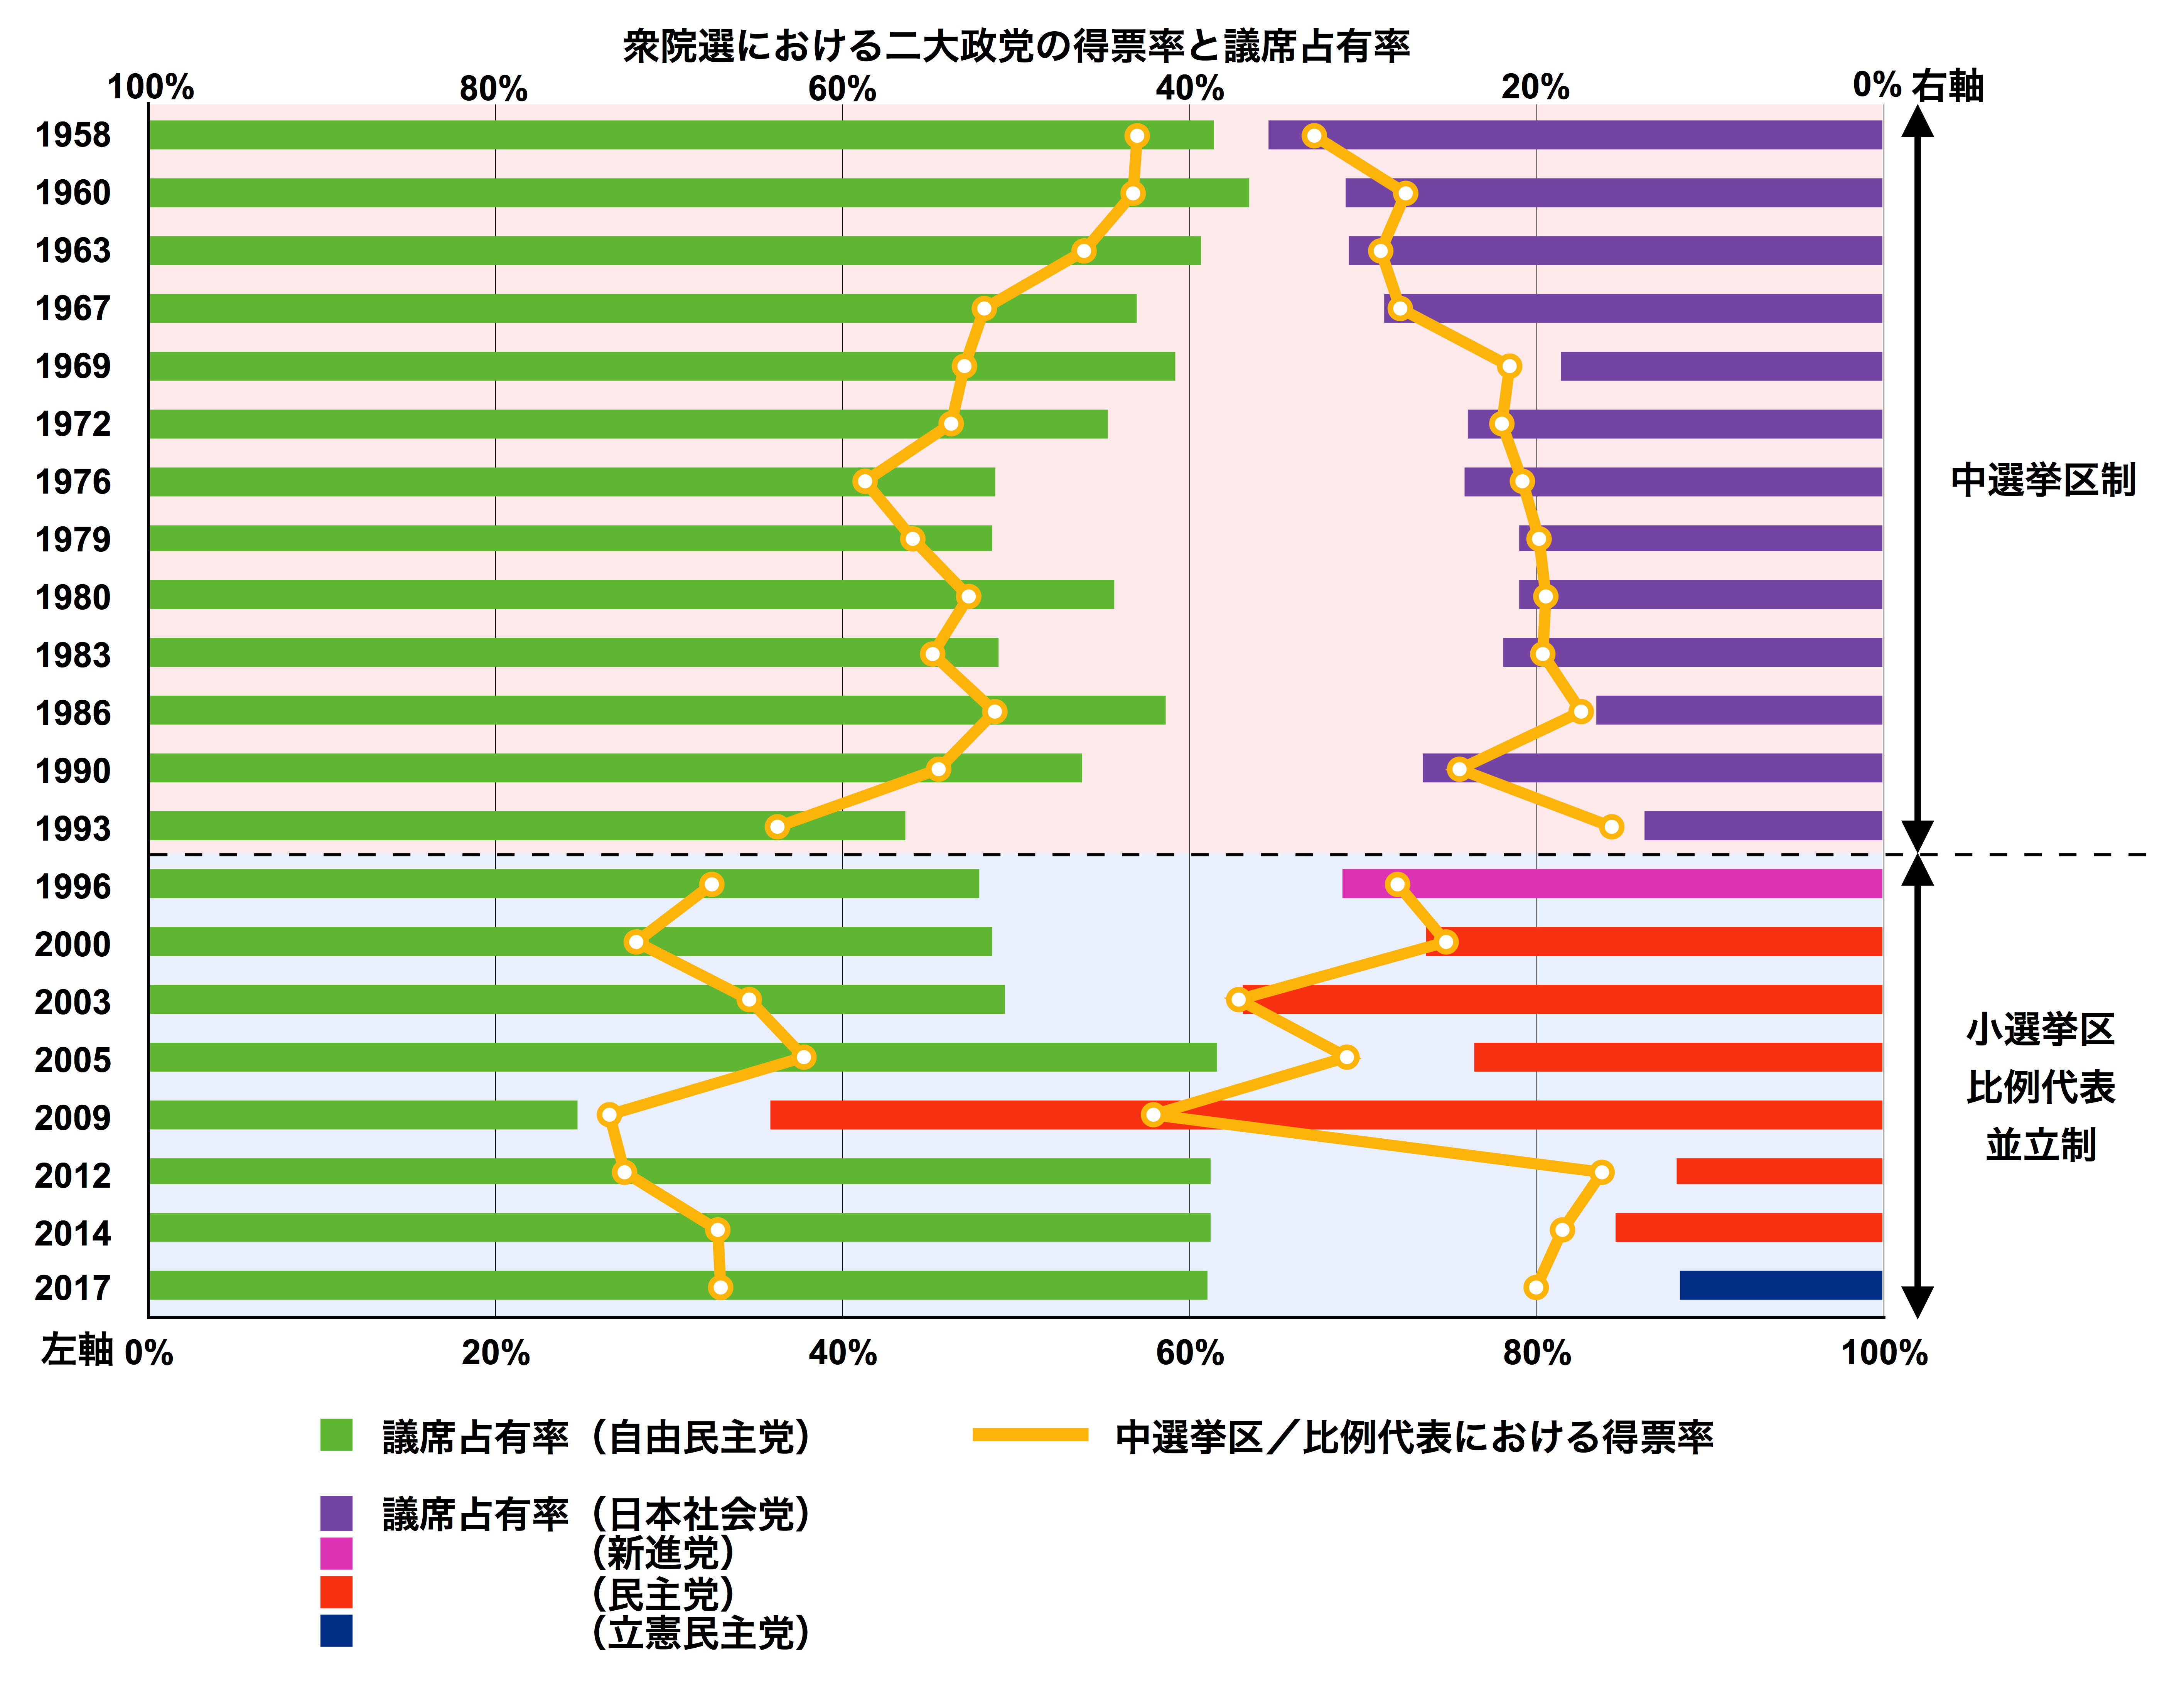
\includegraphics[width=960px]{Two_Major_Parties_in_House_of_Representatives_of_Japan} \caption{衆議院における二大政党の得票率・議席占有率}\label{fig:jpparty}
\end{figure}

出所)\href{https://ja.wikipedia.org/wiki/55\%E5\%B9\%B4\%E4\%BD\%93\%E5\%88\%B6}{Wikipedia}

\begin{itemize}
\item
  政府(≒自民党)、官僚、財界(経団連等)が、政策の(事前)調整を行う構造を「政官財トライアングル」といいます。(図\ref{fig:triangle}参照)

  \begin{itemize}
  \item
    官僚、財界は人の入れ替わりがあっても、組織は永続的です。政府は政権交代があるため本来永続的ではありませんが、自民党の長期政権であったため、官僚、財界とともに長期的な関係を築くことができました\footnote{山岸・ブリントン (2010)のいう\protect\hyperlink{labor}{セカンドチャンス}は、転職の文脈におけるこの状況を示していると解釈できます。}。
  \item
    政府、官僚、財界はそれぞれ「持ちつ持たれつ」の関係です。

    \begin{itemize}
    \item
      企業は同じ産業の企業が集まり、業界団体を構成します。
    \item
      省庁には局(企業の部に相当)やその下に課が存在し、産業ごとに担当する部署を原課・原局といいます。
    \item
      自民党にも産業ごとに政策部会があり、「族議員」と呼ばれます。
    \end{itemize}
  \item
    政府は永田町、官僚は霞が関、企業は丸の内・大手町にあり、すぐに会える距離にあります。
  \item
    高級官僚は退職する際に所管する業界の企業に再就職し、「政官財トライアングル」の連絡係として機能しました。

    \begin{itemize}
    \tightlist
    \item
      この再就職は「天下り」と呼ばれますが、現在、「天下り」は法律で禁止されています。
    \end{itemize}
  \end{itemize}
\end{itemize}

\begin{figure}
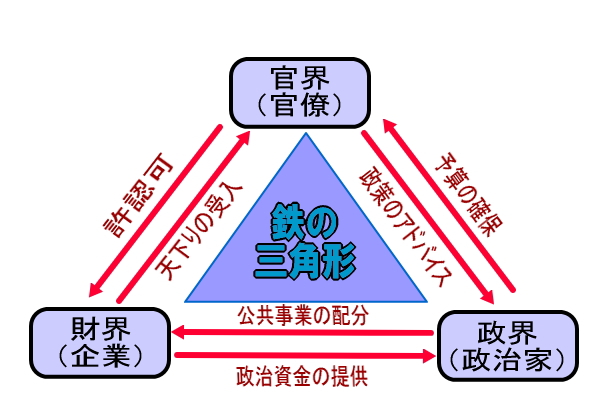
\includegraphics[width=960px]{triangle1} \caption{政官財トライアングル}\label{fig:triangle}
\end{figure}

出所)\href{https://www.seijikeizaijuku.com/naikaku.html}{政治経済塾 (2017)}

\begin{itemize}
\item
  契約書は「最低限のことだけ決めておいて、それ以外(想定外のこと)は互いが協調して話し合いで決めよう」と、簡潔に記載されることが多いです。

  \begin{itemize}
  \item
    最後の方の条項で、「本契約の規定に関する疑義又はこれらの規定に定めのない事項については、甲乙誠意をもって協議の上、解決するものとする。」のような条文が付いている場合が多くあります。
  \item
    このような条項を「誠実協議条項」\footnote{日本は例外です。}といいます。法的には意味がないと考えられるのですが、法制度だけでなく関係性による強制力が機能する長期的関係が背景にあることを示唆する項目といえます。
  \end{itemize}
\end{itemize}

\hypertarget{japan-economy}{%
\subsection{経済システム}\label{japan-economy}}

\begin{itemize}
\item
  日本の経済システムは、政府主導型でした。

  \begin{itemize}
  \item
    政官財トライアングルで調整された政策によって、(繊維産業や電機産業など時代によって変化させた)ターゲット産業を中心に経済成長を図るものです。
  \item
    政府(経済企画庁)が策定した計画にもとづき、通商産業省(現在の経済産業省)が各産業の振興(また円滑な縮小)を目的に策定する政策を\textbf{産業政策}といいます\footnote{将来役員になれるか(日本に比べ)比較的早い段階でわかるので、早期退社し起業する人が多いのがアジアの特徴です。韓国の現状については\href{https://toyokeizai.net/articles/-/473559}{菅野 (2021)}を参考にしてください。}。
  \item
    産業政策には(関税など)保護貿易、研究開発等への補助金、資金調達の援助などが含まれます。
  \end{itemize}
\end{itemize}

\begin{itemize}
\item
  日本企業の特徴は「系列\footnote{学歴重視社会・競争社会は、若年層の失業問題などの社会問題を引き起こしています。中国の現状については\href{https://diamond.jp/articles/-/277433}{王 (2021)}、韓国の現状については\href{https://hbol.jp/pc/189601/}{和場ほか (2019a)}、\href{https://hbol.jp/pc/189810/}{和場ほか (2019b)}を参考にしてください。}」です。日本の高い長期志向(長期的関係)の典型例です。

  \begin{itemize}
  \item
    系列は、個々の企業は独立しているものの、緊密な関係(資本、人事、技術、取引)にある企業群を指します。
  \item
    市場経済の(独立した)各企業よりも近い関係にあるが、単一の企業よりも緩やかな関係です。
  \end{itemize}
\item
  系列には水平的系列と垂直的系列の2種類があります。

  \begin{itemize}
  \item
    水平的系列は、多角化した(戦前の)財閥系(三菱、三井、住友等)企業が、戦後に銀行を中心にまとまったものです。(図\ref{fig:mitsubishi}参照)
  \item
    グループ内の銀行が融資を行う、グループ企業が相互に株式を持ち合って買収を妨げる、毎月社長が会合を持って情報交換するといった特徴があります。
  \end{itemize}
\end{itemize}

\begin{figure}
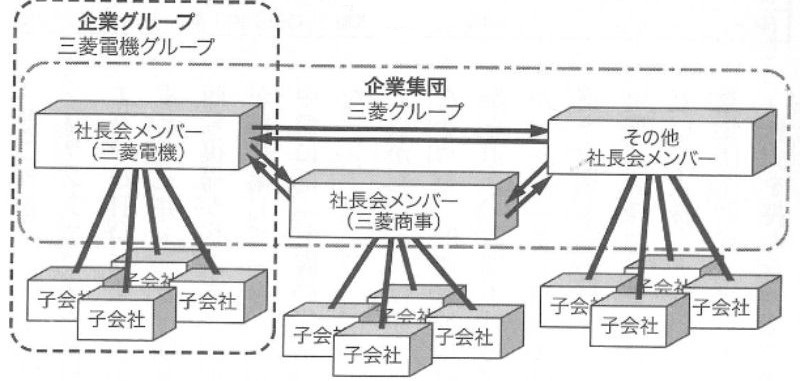
\includegraphics[width=960px]{https://liberal-arts-guide.com/wp-content/uploads/2020/09/Corporate-group-1} \caption{三菱財閥と三菱グループ}\label{fig:mitsubishi}
\end{figure}

出所)\href{https://liberal-arts-guide.com/corporate-group/}{リベラルアーツガイド (2020a)}

注)元資料は、菊池浩之(2017)『三井・三菱・住友・芙蓉・三和・一勧 日本の六大企業集団』KADOKAWA 23頁

\begin{figure}
\includegraphics[width=960px]{https://www.jftc.go.jp/info/nenpou/h06/Img/02070001} \caption{六大企業集団の社長会}\label{fig:bigsix}
\end{figure}

出所)\href{https://www.jftc.go.jp/info/nenpou/h06/02070002.html}{公正取引委員会 (1995)}

\begin{figure}
\includegraphics[width=960px]{https://www.jftc.go.jp/info/nenpou/h10/Img/02070006} \caption{六大企業集団の株式持ち合い}\label{fig:bigsix2}
\end{figure}

出所)\href{https://www.jftc.go.jp/info/nenpou/h10/02070001.html}{公正取引委員会 (1999)}

\begin{itemize}
\item
  垂直的系列は、大企業が部品を供給する関係会社をまとめた(日立、松下→パナソニック、トヨタ等)ものです。

  \begin{itemize}
  \item
    親会社が子会社を、子会社が孫会社の株式を保有する構造になります。
  \item
    水平的系列の各企業も垂直的系列をもっています(例:三菱重工業が三菱重工業グループを形成)。
  \item
    日立製作所のCMは日立グループの紹介になっています。
  \end{itemize}
\end{itemize}

\begin{itemize}
\item
  日本経済は、効率的な部門と非効率な部門が存在する二重構造になっています。

  \begin{itemize}
  \tightlist
  \item
    国内向けサービス業(通信・小売・金融)や農業が非効率で国際競争力が低い一方で、輸出向け製造業(自動車、電機、機械)は国際競争力が高く、世界的大企業もあります。
  \end{itemize}
\item
  バブル経済の絶頂期には日本企業は銀行業が巨大化し世界時価総額ランキングの上位を多く占めていましたが、現在では上位50社にトヨタ自動車がランクされるのみです。(図\ref{fig:value}参照)
\end{itemize}

\begin{figure}
\includegraphics[width=960px]{https://media.startup-db.com/wp/wp-content/uploads/2019/07/1-min-1} \caption{グローバル時価総額ランキングー平成元年と平成31年ー}\label{fig:value}
\end{figure}

出所)\href{https://media.startup-db.com/research/marketcap-global}{STARTUP DB (2019)}

\begin{itemize}
\item
  労働組合は企業別労働組合で、労使がよく協調する点が特徴です。

  \begin{itemize}
  \item
    戦後、労働運動が激しい時期がありましたが、1970年代以降激しい対立は少なくなりました。
  \item
    労働争議で失われる時間は先進国のなかで最少となっています。(図\ref{fig:strike}参照)
  \end{itemize}
\end{itemize}

\begin{figure}
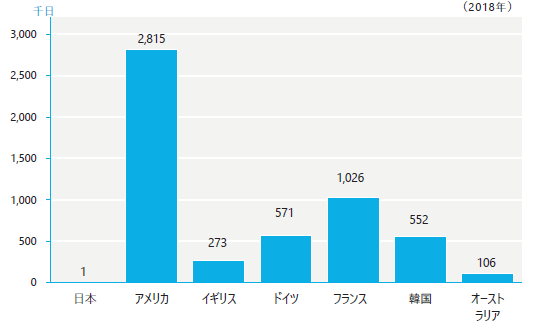
\includegraphics[width=960px]{strike} \caption{労働争議による労働損失日数}\label{fig:strike}
\end{figure}

出所)\href{https://www.jil.go.jp/kokunai/statistics/databook/2019/07/d2019_G7-2.pdf}{労働政策研究・研修機構 (2019, p.264)}

{\textbf{参考文献}}

Meyer, E. (2014). The Culture Map: Breaking Through the Invisible Boundaries of Global Business. PublicAffairs.(日本語版 樋口武志(訳)・田岡恵(監訳)(2015)『異文化理解力』英治出版.)

\href{https://media.startup-db.com/research/marketcap-global}{STARTUP DB (2019)「平成最後の時価総額ランキング。日本と世界その差を生んだ30年とは?」}

Weber, Max (1905). Die protestantische Ethik und der Geist des Kapitalismus. (日本語版 大塚久雄(訳)(1989)『プロテスタンティズムの倫理と資本主義の精神』岩波文庫.)

\href{https://u-note.me/note/47506034}{U-NOTE編集部 (2021) 「どちらが美徳?日本人に根づく「恥の文化」と諸外国の「罪の文化」」}

\href{https://ja.wikipedia.org/wiki/55\%E5\%B9\%B4\%E4\%BD\%93\%E5\%88\%B6}{Wikipedia「55年体制」}

\href{https://www.jftc.go.jp/info/nenpou/h06/02070002.html}{公正取引委員会 (1995)『平成6年度 公正取引委員会年次報告』}

\href{https://www.jftc.go.jp/info/nenpou/h10/02070001.html}{公正取引委員会 (1999)『平成10年度 公正取引委員会年次報告』}

\href{https://www.seijikeizaijuku.com/naikaku.html}{政治経済塾 (2017)「6時間目:内閣」}

\href{https://www.soumunomori.com/column/article/atc-115077/}{総務の森 (2010) 「契約書の基礎知識 誠実協議条項とは」}

寺西重郎 (2018)『日本型資本主義』中公新書2502.

\href{https://www.qingdao.cn.emb-japan.go.jp/jp/publicrelations/index_150917.html}{遠山茂 (2015)「儒教思想の日本への影響」在青島日本国総領事館}

山岸俊男・ブリントン,メアリー・C (2010)『リスクに背を向ける日本人』講談社現代新書2073.

\href{https://liberal-arts-guide.com/corporate-group/}{リベラルアーツガイド (2020a)「【企業集団とは】意味から財閥との違いまでわかりやすく解説」}

\href{https://www.jil.go.jp/kokunai/statistics/databook/2019/index.html}{労働政策研究・研修機構 (2019)『データブック国際労働比較2019』}

\hypertarget{japan-manager}{%
\section{日本企業の経営者}\label{japan-manager}}

\begin{itemize}
\item
  本節では、日本企業の経営者に関連する項目を整理します。

  \begin{itemize}
  \item
    まず、日本企業の経営者のキャリア形成のプロセス、\protect\hyperlink{japan-selection}{選抜・移動}を整理します。
  \item
    次に、日本企業の経営者の\protect\hyperlink{japan-payment}{報酬}について、概要を整理します。
  \item
    最後に、日本企業の経営者の教育的背景(学歴)や、経営学の\protect\hyperlink{japan-education}{教育}の位置付けについて整理します。
  \end{itemize}
\end{itemize}

\hypertarget{japan-selection}{%
\subsection{選抜・移動}\label{japan-selection}}

\begin{itemize}
\item
  \href{https://www.strategyand.pwc.com/jp/ja/publications/2018_ceo-data-media-release-jp.pdf}{Strategy\& (2019)}が行った、世界の上場企業における時価総額の上位2,500社を対象にした調査によると、日本企業の経営者(最高経営責任者CEO:Chief Executive Officer)の平均像は、以下の通りです。 \protect\hyperlink{us-selection}{アメリカ} \protect\hyperlink{asia-selection}{アジア}

  \begin{itemize}
  \item
    2018年に就任したCEOの年齢の中央値は60才です。

    \begin{itemize}
    \item
      Edfelt (2010, pp.240-241)によると、日本企業は以下の特徴があります。

      \begin{itemize}
      \item
        50代で常務になり、(専務を経て)社長に就任するのは平均で59才
      \item
        社長として6.3年経営し、その後2/3が会長になる
      \item
        業績不振によって退任を強いられることは少ない
      \end{itemize}
    \end{itemize}
  \item
    内部昇格したCEOが97\%で、外部招聘のCEOが3\%でした(図\ref{fig:JPceo1}参照)。

    \begin{itemize}
    \tightlist
    \item
      新任CEOの18\%が他企業での職務経験があります。
    \end{itemize}
  \item
    海外での勤務経験を有するCEOは21\%でした(図\ref{fig:JPceo2}参照)。
     

    \begin{itemize}
    \tightlist
    \item
      世界平均レベル(33\%)に比べると低い水準です。
    \end{itemize}
  \item
    新任CEOの100\%が日本国籍でした。
  \item
    新任CEOの女性比率は0\%でした。

    \begin{itemize}
    \item
      デロイトトーマツグループと三井住友信託銀行とによる上場企業970社を対象にした調査(2021年)によると、「取締役に女性・外国人とも登用していない企業は48\%、女性取締役がゼロは51\%だった。2020年の調査(902社)でそれぞれ57\%、60\%だったのに比べて女性・外国人の登用が進んだものの、なお半数の企業の取締役会が日本人男性のみで運営」されていました\footnote{日本経済新聞朝刊 2021年11月21日「女性・外国人取締役、主要企業の半数でゼロ」}。
       
    \item
      \href{https://www.tdb.co.jp/report/watching/press/p210805.html}{帝国データバンク (2021)}によると、日本企業の女性管理職(注:CEOではない)の平均割合は過去最高となったものの 8.9%にとどまりました。
    \item
      政府は2003年に「\textbf{2020年}までに女性管理職の割合を30\%に」との期限付き目標を掲げましたが、実現が見通せず、2020年12月に「2020年代の可能な限り早期に」と改めています\footnote{\href{https://www.nikkei.com/article/DGXZQOCC1454K0U1A510C2000000/}{日本経済新聞電子版 2021年5月15日「女性の管理職比率とは 米欧先行、日本は10\%台」}}。
    \item
      \href{https://www.meti.go.jp/press/2022/05/20220531001/20220531001-1.pdf}{経済産業省 (2022, p.47)}によると、日本(2020年)の役員の女性比率は6\%、管理職の女性比率は15\%でした(図\ref{fig:femaleexective}参照)。
    \end{itemize}
  \end{itemize}
\end{itemize}

\begin{figure}
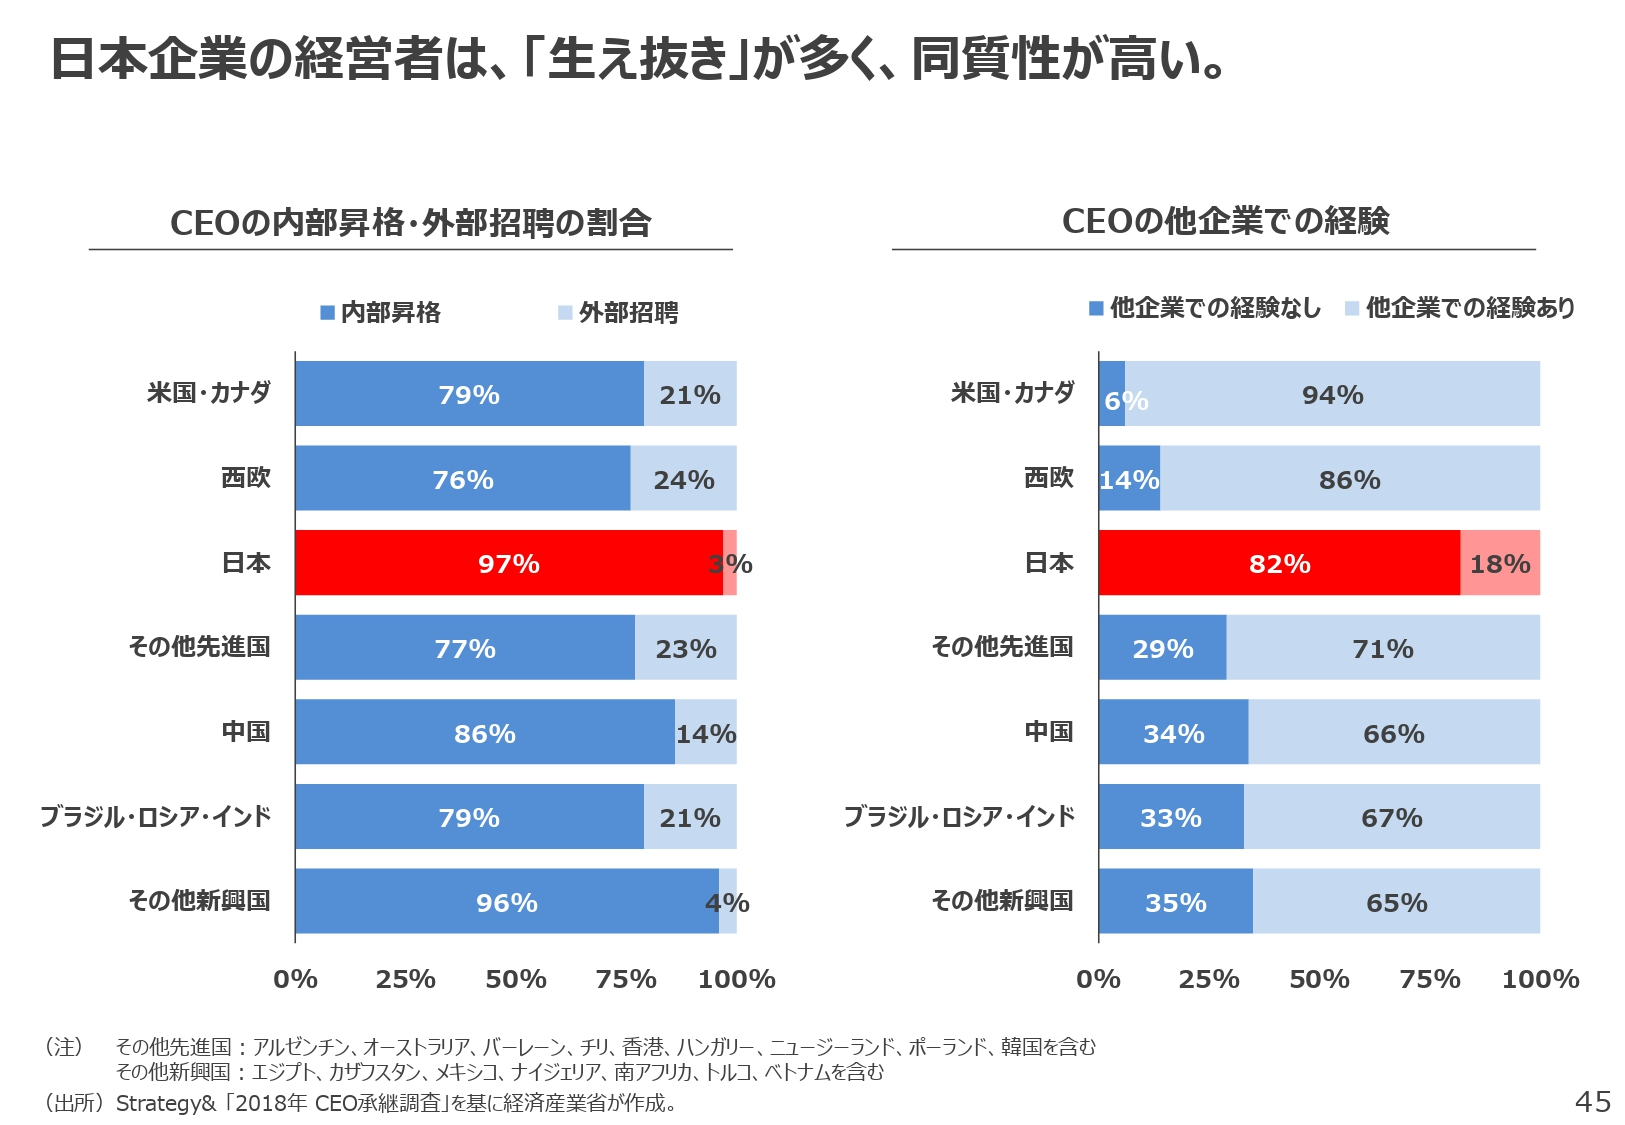
\includegraphics[width=960px]{miti_page-0046} \caption{CEOの内部昇格・外部招聘の割合/CEOの他企業での経験}\label{fig:JPceo1}
\end{figure}

出所)\href{https://www.meti.go.jp/press/2022/05/20220531001/20220531001-1.pdf}{経済産業省 (2022, p.45)}

\begin{figure}
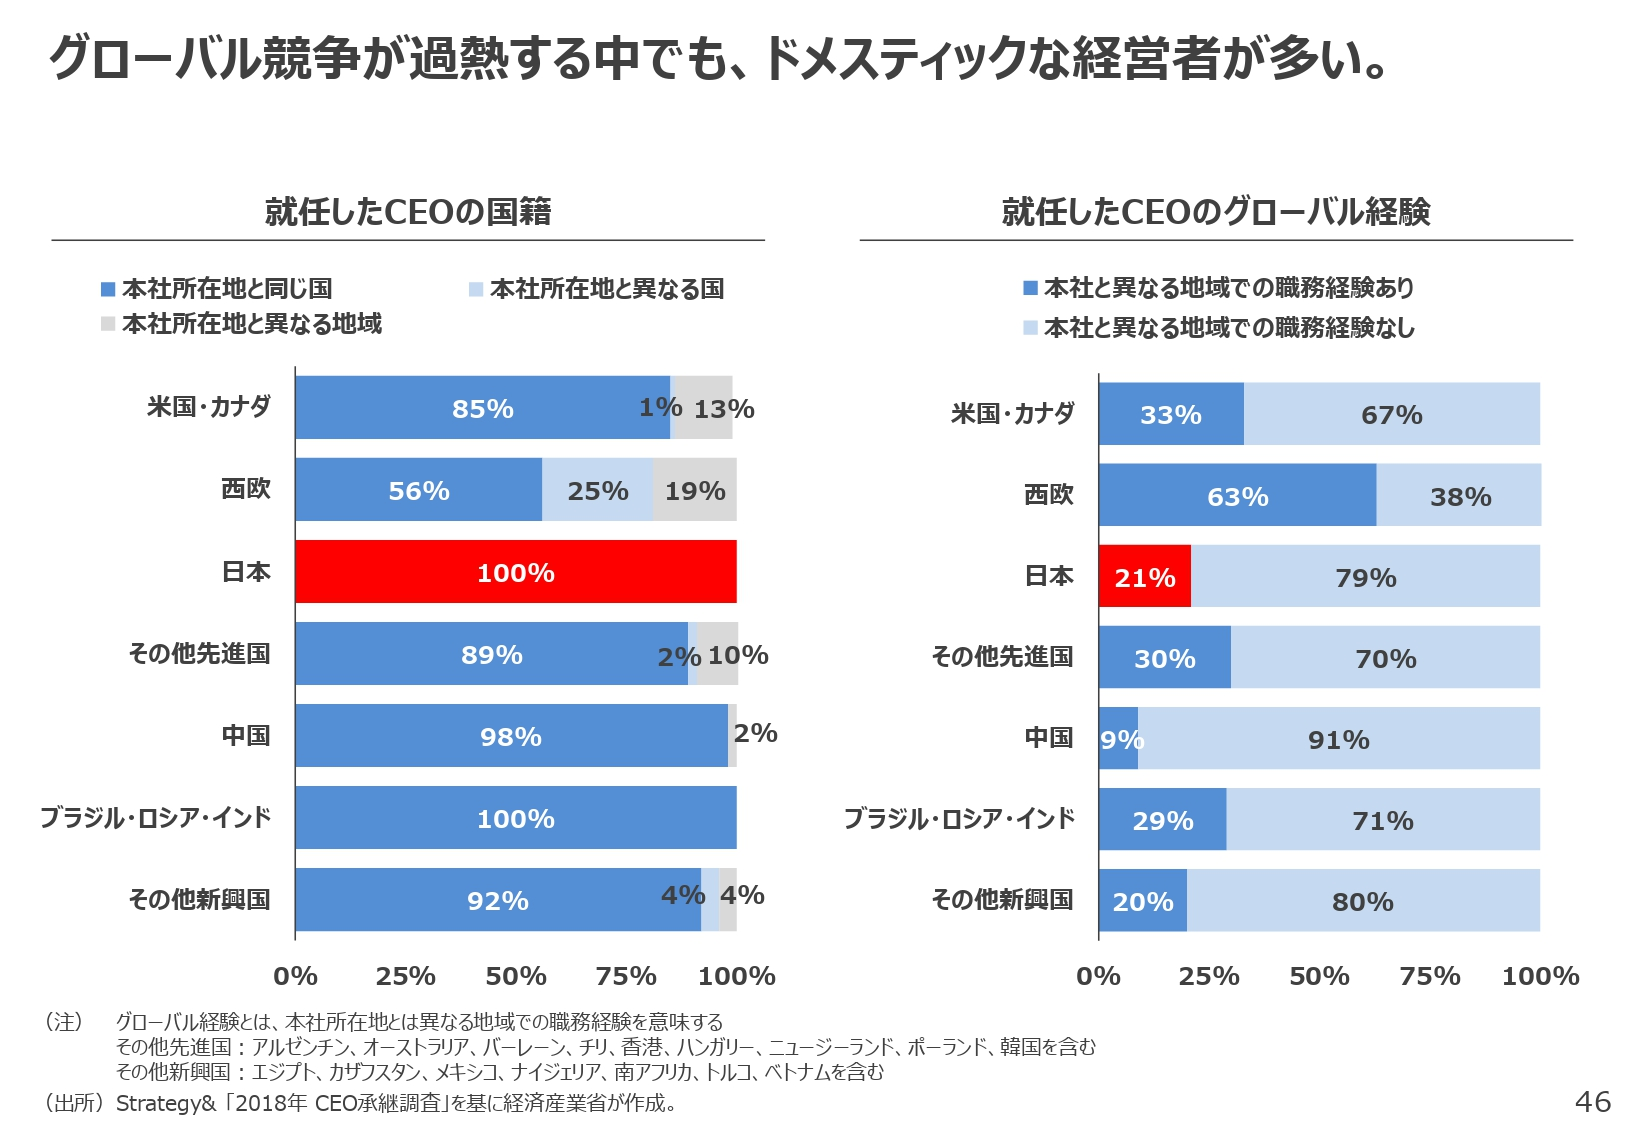
\includegraphics[width=960px]{miti_page-0047} \caption{就任したCEOの国籍/就任したCEOのグローバル経験}\label{fig:JPceo2}
\end{figure}

出所)\href{https://www.meti.go.jp/press/2022/05/20220531001/20220531001-1.pdf}{経済産業省 (2022, p.46)}

\begin{figure}
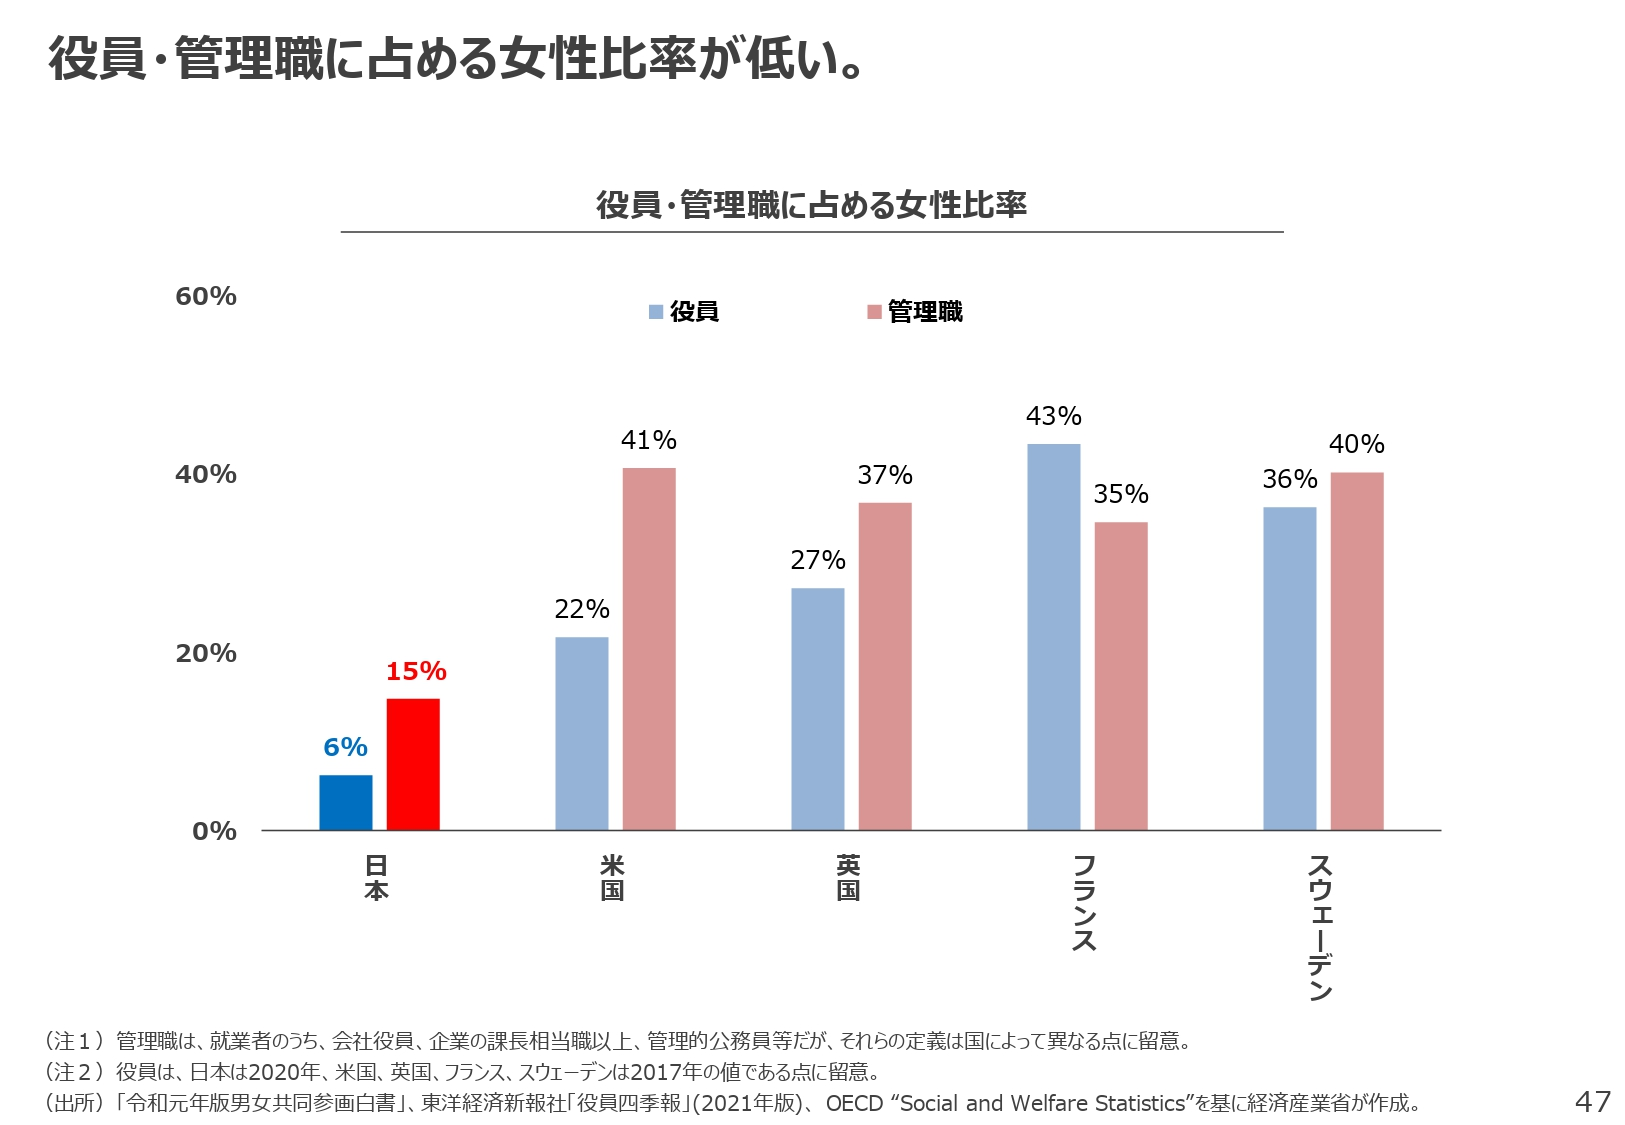
\includegraphics[width=960px]{miti_page-0048} \caption{役員・管理職に占める女性比率}\label{fig:femaleexective}
\end{figure}

出所)\href{https://www.meti.go.jp/press/2022/05/20220531001/20220531001-1.pdf}{経済産業省 (2022, p.47)}

\begin{itemize}
\item
  新任CEOの0\%がMBA(経営学修士)保有者です。

  \begin{itemize}
  \item
    世界平均(33\%)を大きく下回ります。
  \item
    理系出身は大学院修了(修士)も一般的ですが、文系出身は大学卒業\footnote{CEOの学歴として、「大卒」は国際的には低学歴といえます。}が多いです。
  \end{itemize}
\end{itemize}

\begin{itemize}
\tightlist
\item
  小熊 (2019, p.6)は、経団連\footnote{経団連については、\href{https://gakumado.mynavi.jp/style/articles/46464}{マイナビ (2020) ``「経団連」とは? 今さら聞けないその言葉の意味・役割・取り組みを解説''}などを参考にしてください。}正副会長のプロフィール(表\ref{tab:keidanren})を参考にして、本節で述べた日本企業の特徴を以下の通りまとめています。
\end{itemize}

\begin{quote}
\begin{enumerate}
\def\labelenumi{\arabic{enumi}.}
\tightlist
\item
  まず、学歴が重要な指標となっている。ただし重要なのは学校名であり、何を学んだかではない。\\
\item
  つぎに、年齢や勤続年数が、重要な指標となっている。ただしそれは、1つの企業での勤続年数であって、他の企業での職業経験は評価されない。\\
\item
  その結果、都市と地方という対立が生じる。何を学んだかが重要なら、必ずしも首都圏の有名大学である必要はない。\\
\item
  そして、女性と外国人が不利になる。女性は結婚と出産で、勤続年数が中断されがちだ。また他国企業での職業経験が評価されないなら、外国人は入りにくい。
\end{enumerate}
\end{quote}

\begin{table}

\caption{\label{tab:keidanren}日本経団連正副会長19名(2018年6月)のプロフィール}
\centering
\begin{tabular}[t]{>{\raggedright\arraybackslash}p{6em}|>{\raggedright\arraybackslash}p{6em}|l|>{\raggedright\arraybackslash}p{6em}|>{\raggedright\arraybackslash}p{6em}|>{\raggedright\arraybackslash}p{6em}|>{\raggedright\arraybackslash}p{6em}}
\hline
国籍 & 性別 & 創業者orプロorサラリーマン & 転職経験 & 最年少 & 出身校 & 海外経験\\
\hline
全員日本人 & 全員男性 & 全員サラリーマン経営者 & 全員なし & 62歳 & 東大(12人) & 駐在経験あり(7人)\\
\hline
\end{tabular}
\end{table}

出所)日本経済新聞\footnote{日本経済新聞朝刊 2018年6月18日「変わる経団連、変われぬ経団連」}、日本産業新聞\footnote{日経産業新聞 2018年6月22日「経団連 この恐るべき同質集団」}

\begin{itemize}
\item
  学歴重視の結果、日本企業の経営者は同質性が高く、ダイバーシティの面で遅れていると指摘されています。
\item
  終身雇用の一方で、海外企業比べ昇進が遅いのが特徴です。

  \begin{itemize}
  \item
    海外企業では社員を競わせ、昇進できなかった社員は退社していきます(up or out)。
  \item
    日本企業は定年退職まで企業にいるため、昇進が遅れた社員がやる気をなくして働く期間が長くなります。そこで同期入社でできるだけ差が生まれないよう昇進を遅らせます。
  \end{itemize}
\end{itemize}

\begin{table}

\caption{\label{tab:promotion}課長・部長への昇進年齢}
\centering
\begin{tabular}[t]{l|l|l}
\hline
国 & 課長 & 部長\\
\hline
中国 & 28.5歳 & 29.8歳\\
\hline
インド & 29.2歳 & 29.8歳\\
\hline
タイ & 30.0歳 & 32.0歳\\
\hline
米国 & 34.6歳 & 37.2歳\\
\hline
日本 & 38.6歳 & 44.0歳\\
\hline
\end{tabular}
\end{table}

出所)\href{https://www.meti.go.jp/press/2022/05/20220531001/20220531001-1.pdf}{経済産業省 (2022, p.36)}

\begin{itemize}
\item
  移動の少なさは、終身雇用によって転職が経済的に不利であることや(そのために)不確実性回避が高くなっていることから解釈できます。

  \begin{itemize}
  \tightlist
  \item
    「現在の勤務先で働き続けたい」と考える人は少ない(図\ref{fig:change1}参照)一方で、「転職や起業」の意向を持つ人も少ない(図\ref{fig:change2}参照)という調査結果が出ています。
  \end{itemize}
\end{itemize}

\begin{figure}
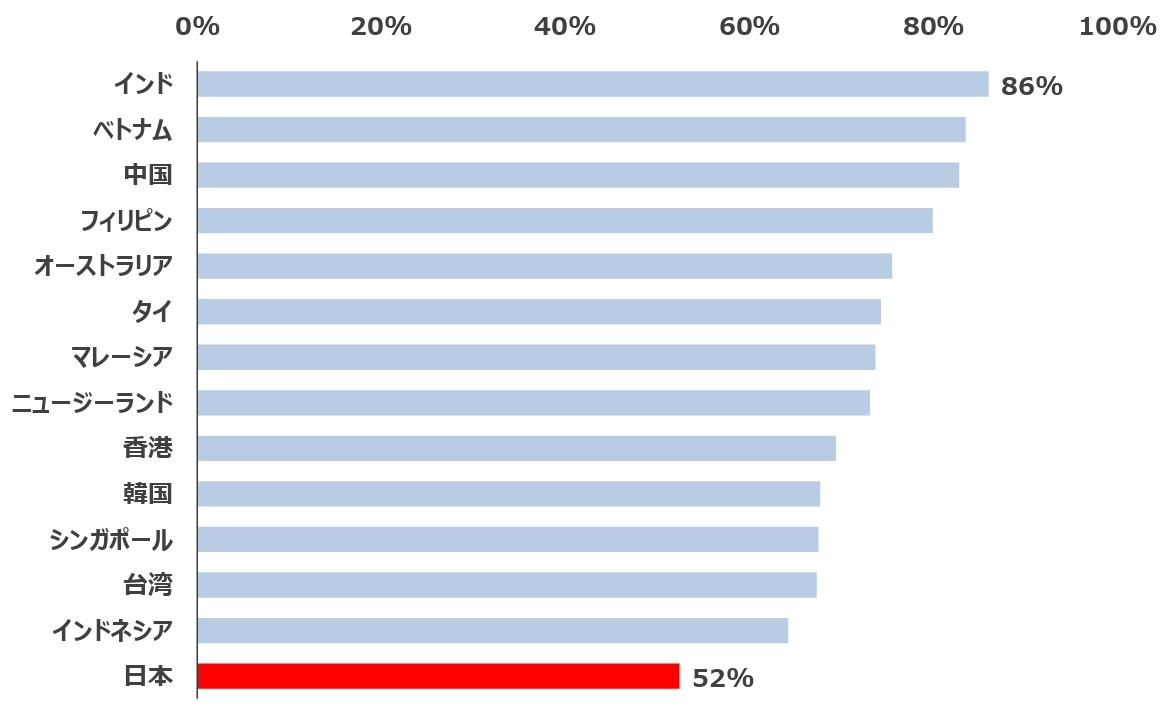
\includegraphics[width=960px]{miti_page-0035} \caption{現在の勤務先で継続して働きたい人の割合}\label{fig:change1}
\end{figure}

出所)\href{https://www.meti.go.jp/press/2022/05/20220531001/20220531001-1.pdf}{経済産業省 (2022, p.34)}

\begin{figure}
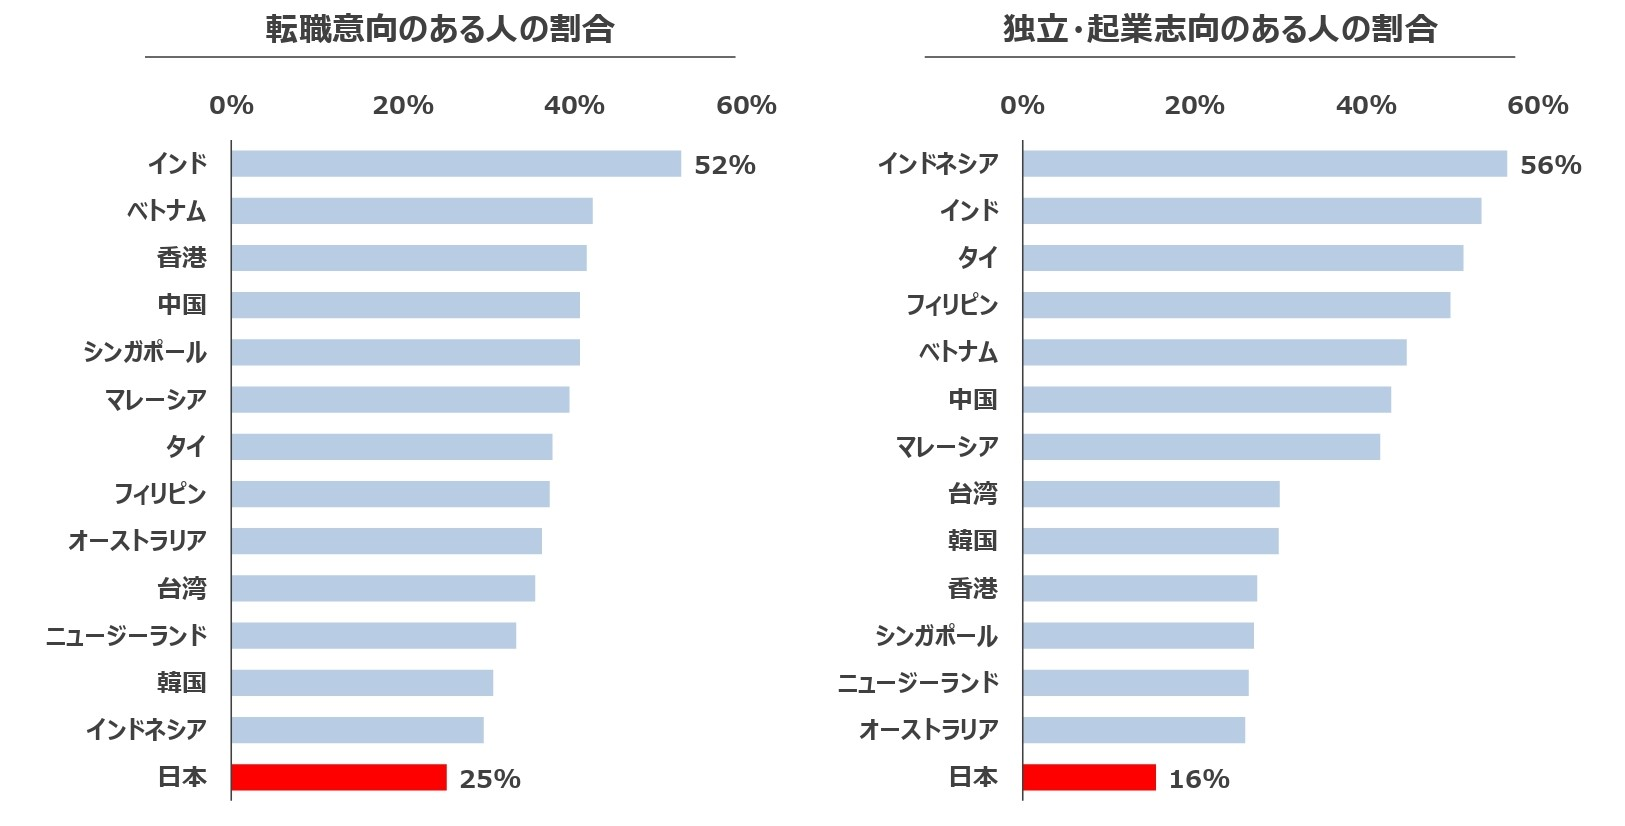
\includegraphics[width=960px]{miti_page-0036} \caption{転職意向のある人の割合/独立・起業志向のある人の割合}\label{fig:change2}
\end{figure}

出所)\href{https://www.meti.go.jp/press/2022/05/20220531001/20220531001-1.pdf}{経済産業省 (2022, p.35)}

\hypertarget{japan-payment}{%
\subsection{報酬}\label{japan-payment}}

\begin{itemize}
\item
  \ref{us-payment}で見たとおり、日本企業CEOの報酬(2020年度)の中央値は1.8億円でした。
\item
  \href{https://toyokeizai.net/articles/-/620775}{東洋経済新報社 (2022)}によれば、2億円以上の報酬は267人いました。

  \begin{itemize}
  \item
    外国人のCEOは少ないですが、役員は多く見られるようになりました。
  \item
    業績連動ボーナスを実施する企業は少ないですが、増えつつあります\footnote{日本経済新聞朝刊 2020年7月19日「社長の報酬、日米で格差12倍に 19年度 業績連動部分少なく」によると、自社の現物株を報酬として付与する企業が、2020年6月末時点で800社超と過去1年間で5割増えまし
      た。日本では報酬全体の57\%が固定給ですが、アメリカではわずか9\%です。}。
  \end{itemize}
\end{itemize}

\begin{itemize}
\item
  \href{https://toyokeizai.net/articles/-/397196}{東洋経済新報社 (2020)}によると、ペイレシオが高い企業3社は武田薬品工業55.67倍、ユニバーサルエンターテイメント47.66倍、ソフトバンク43.35倍となっています。

  \begin{itemize}
  \tightlist
  \item
    ペイレシオは先進国で最も低いです。
  \end{itemize}
\item
  日本企業は終身雇用かつ年功賃金のため、転職が少ないです。

  \begin{itemize}
  \item
    年功賃金では、仕事の貢献度と受け取る賃金が異なるため、中途退社が不利な賃金体系となります(図\ref{fig:jpwage}参照)。
  \item
    年功賃金は海外にもありますが、日本はその傾向が強いです(図\ref{fig:wages}参照)。
  \end{itemize}
\end{itemize}

\begin{figure}
\includegraphics[width=960px]{https://www.hj.sanno.ac.jp/cp/feature/img/20191224-01/20191224-01-01} \caption{「賃金カーブ」と「貢献度曲線」の関係}\label{fig:jpwage}
\end{figure}

出所)\href{https://www.hj.sanno.ac.jp/cp/feature/201912/24-01.html}{産業能率大学総合研究所 (2021)}

\begin{figure}
\includegraphics[width=960px]{wages} \caption{賃金カーブの国際比較}\label{fig:wages}
\end{figure}

出所)\href{https://www.nikkei.com/article/DGXKZO46883220S9A700C1EA2000/}{日本経済新聞電子版 2019年7月3日「年功序列型の賃金とは 日本型経営「三種の神器」」}

\hypertarget{japan-education}{%
\subsection{教育}\label{japan-education}}

\begin{itemize}
\item
  大企業・政府は有名大学から新規学卒者を大量に採用します。

  \begin{itemize}
  \item
    受験によって選抜が済んでいると考えています。
  \item
    個人の資質(責任感、規律等)を重視し、大学の専攻はさほど重要視しません。
  \item
    小熊 (2019)は、上掲の日経新聞記事が「卒業した大学名は詳細に記されているが、学部や専攻については何も述べていない」ことを指摘し、日本社会は「何を学んだかが重要でない学歴\footnote{冨山和彦氏は対談の中で「そうですね。合格歴ですよね。濁点が違っています。「高学歴」じゃなくて「合格歴主義」(笑)。」といっています。\href{https://gendai.ismedia.jp/articles/-/71570?page=5}{小野・冨山 (2020)}}重視」であるとしています。
  \end{itemize}
\end{itemize}

\begin{itemize}
\item
  「仕事」をきちんと決めておいてそれに「人」を当てはめるやり方の欧米諸国に対し、「人」を中心に管理が行われ、「人」と「仕事」の結びつきはできるだけ自由に変えられるようにしておくのが日本の特徴です(濱口 (2013, p.35))。

  \begin{itemize}
  \item
    そこで求められるのは、「いかなる職務をも遂行しうる潜在能力」となります。
  \item
    企業は採用に当たって「新規学卒者の「能力」の代理指標としてその学歴水準、それもどのランクの大学に入れたか(中略)という指標を採用(濱口 (2013, p.126))」します。
  \item
    情報の経済学におけるシグナリングという概念を使うと、学歴重視には合理性があるとされます。
  \end{itemize}
\item
  大卒の1/5は経済・商学系(アメリカと同様)です。

  \begin{itemize}
  \tightlist
  \item
    しかし(生産)現場を重視し、学問としての経営学を重視しない傾向があります。
  \end{itemize}
\item
  経済・商学系学部卒の16人に1人がビジネススクールに進学します(Edfelt (2010, p.242))。

  \begin{itemize}
  \item
    ただし、MBAが出世や昇給の近道となっていません。
  \item
    むしろ、文系で修士号や博士号を取得していると、逆に出世しにくい面があります。「ムラ社会だと修士号や博士号を持っていると「異端」に位置づけられて、「本流」から外されてしまうわけです(\href{https://gendai.ismedia.jp/articles/-/71570?page=5}{小野・冨山 (2020)})」
  \end{itemize}
\item
  企業で必要な技能には「一般的技能」と「企業特殊的技能」の2種類があると言われています。

  \begin{itemize}
  \item
    「一般的技能」とは、転職して他社に移っても転用可能な技能です。語学、簿記、ITスキルなどが挙げられます。

    \begin{itemize}
    \tightlist
    \item
      「一般的技能」を修得すると転職する際に評価されるので、従業員は転職が容易になります。そのため企業が「一般的技能」の教育訓練(を負担)することはあまりありません(図\ref{fig:HRinvestment}参照)。
    \end{itemize}
  \item
    「企業特殊的技能」とは、その企業内でしか使えない技能です。企業独特の仕事のやり方、社内手続きルールのほか、職場における良好な人間関係などが挙げられます。

    \begin{itemize}
    \item
      「企業特殊的技能」を習得しても、転職する際には評価されない(できない)ので、転職が賃金増加につながらない傾向があります。
    \item
      終身雇用を前提とすると、従業員が「企業特殊的技能」を習得することは合理的となります。
    \end{itemize}
  \end{itemize}
\end{itemize}

\begin{figure}
\includegraphics[width=960px]{miti_page-0041} \caption{転職意向のある人の割合/独立・起業志向のある人の割合}\label{fig:HRinvestment}
\end{figure}

出所)\href{https://www.meti.go.jp/press/2022/05/20220531001/20220531001-1.pdf}{経済産業省 (2022, p.40)}

\begin{itemize}
\item
  「企業特殊的技能」に関わる社内教育は充実しています。

  \begin{itemize}
  \tightlist
  \item
    濱口 (2013, p.97)は、その理由を次のように説明しています。
  \end{itemize}
\end{itemize}

\begin{quote}
「人」が先にあり、その人にすぐにできるとは限らない「仕事」を当てはめるというやり方ですから、その「仕事」のやり方を社内で学ぶという仕組みがなければ、うまく回っていきません。つまり、仕事に関する教育訓練の仕組みが、社内教育訓練中心の仕組みにならざるを得ないということです。
\end{quote}

\begin{itemize}
\tightlist
\item
  日本では企業が事業構造を変化させるのに伴って、従業員を再教育し成長職種に配置転換させます\footnote{日本経済新聞朝刊 2021年7月7日「工場従業員にDX教育 キヤノン 成長職種へ配置転換」}。労働者が自ら大学(院)でスキルを学び直し転職するアメリカとは対照的です。
\end{itemize}

{\textbf{参考文献}}

Edfelt, Ralph B. (2010). Global Comparative Management. SAGE.

\href{https://www.strategyand.pwc.com/jp/ja/publications/2018_ceo-data-media-release-jp.pdf}{Strategy\& (2019)「2018年 CEO 承継調査」}

\href{https://www.meti.go.jp/press/2022/05/20220531001/20220531001-1.pdf}{経済産業省 (2022)「未来人材ビジョン」}

小熊英二 (2019)『日本社会のしくみ』講談社現代新書2528.

\href{https://gendai.ismedia.jp/articles/-/71570?imp=0}{小野一起・冨山和彦 (2020) 「日本企業で出世する人たち、じつは「超低学歴」ばかりになっていた\ldots!」マネー現代}

\href{https://www.hj.sanno.ac.jp/cp/feature/201912/24-01.html}{産業能率大学総合研究所 (2021) 「賃金を切り口とした年功序列型人事制度の検証」}

\href{https://www.tdb.co.jp/report/watching/press/pdf/p210805.pdf}{帝国データバンク (2021)「女性登用に対する企業の意識調査(2021年)」}

\href{https://toyokeizai.net/articles/-/397196}{東洋経済新報社 (2020)「社員と役員の「年収格差」ランキングTOP500」東洋経済ONLINE}

\href{https://toyokeizai.net/articles/-/453483}{東洋経済新報社 (2021)「「年収1億円超」の上場企業役員ランキングTOP500」東洋経済ONLINE}

濱口桂一郎 (2013)『若者と労働』中公新書ラクレ465.

\hypertarget{japan-management}{%
\section{日本企業のマネジメント}\label{japan-management}}

\begin{itemize}
\item
  本節では、日本企業のマネジメントに関連する項目を整理します。

  \begin{itemize}
  \item
    まず、日本企業の\protect\hyperlink{japan-plan}{計画}を整理します。
  \item
    次に、日本企業の\protect\hyperlink{japan-organization}{組織化}について、概要を整理します。
  \item
    次に、日本企業の\protect\hyperlink{japan-command}{指揮・調整}について、概要を整理します。
  \item
    最後に、日本企業の\protect\hyperlink{japan-control}{統制}について、概要を整理します。
  \end{itemize}
\end{itemize}

\hypertarget{japan-plan}{%
\subsection{計画}\label{japan-plan}}

\begin{itemize}
\item
  日本企業は欧米企業と比べ長期計画は厳密でない一方、経営理念が強く働いています。

  \begin{itemize}
  \item
    経営者の任期が長くないため、(任期を超える)長期計画を策定するよりも、創業者の経営理念(ビジョン)で経営の方向性を示しています。
  \item
    短期・中期計画では、綿密な計画を立てます。
  \end{itemize}
\item
  欧米企業よりも、海外の動向に関する情報収集に熱心だとされています。

  \begin{itemize}
  \item
    旧財閥系の水平的系列では、総合商社を始めとしてグループ各社が国内外で収集した情報を社長会(図\ref{fig:bigsix}参照)を通じて共有します。
  \item
    日本貿易振興会(JETRO)は、国際経済の調査や市場動向に関する情報を収集しています。中小企業は日本貿易振興会(JETRO)を通じてこれらの情報を入手でき、また海外進出について相談することができます。
  \end{itemize}
\item
  長期計画がないことや情報収集に熱心という特徴は、日本企業の強みにも関連します。

  \begin{itemize}
  \item
    とくに高度経済成長期の日本製品は、欧米先進国の模倣でした。独特な製品や戦略がある企業は例外でした。
  \item
    日本製品が競争力を持ったのは、絶え間ないカイゼン\footnote{カイゼン(改善)といった企業内活動は英語圏にないため、kaizenと英語になっています。\href{https://www.ldoceonline.com/jp/dictionary/kaizen}{ロングマン現代英英辞典}}\footnote{カイゼンについては、\href{https://toyokeizai.net/articles/-/202227}{岡内 (2017)}などを参考にしてください。}(コスト削減・品質向上)、柔軟な生産体制、市場化への時間短縮によるものです。
  \item
    つまり、差別化を生み出す戦略・長期計画よりも、海外市場動向(新製品)の情報収集や、コスト削減・品質向上を実現する短期の生産・販売計画に重心が置かれていました。
  \end{itemize}
\end{itemize}

\hypertarget{japan-organization}{%
\subsection{組織化}\label{japan-organization}}

\begin{itemize}
\item
  日本の大企業の多くは事業部制をとっています。事業部を分社化し、経営本部が持株会社(〇〇ホールディングス)として子会社を統括する形態も増えています。
\item
  日本企業の組織の特徴は、その柔軟性です。

  \begin{itemize}
  \item
    欧米のように「職務記述書」で「仕事」の内容、範囲、責任、権限などが規定されておらず、入社後数年ごとに人事ローテーションが行われます。
  \item
    この人事ローテーションによって、社員誰もが複数の経験・スキルを身につけるようになります。製造現場で複数の工程を担当できる工員を「多能工」と呼びます。
  \item
    複数の経験・スキルを身につけていることから、社員は組織を越えて協力することができ、これが日本企業の強みにつながっています。
  \item
    協力の一方で責任も分担されるといったデメリットも生じます。

    \begin{itemize}
    \tightlist
    \item
      柔軟な組織では役割分担が曖昧なため、「共同責任は無責任」となりがちです。
    \end{itemize}
  \end{itemize}
\item
  垂直的系列におけるグループ各社は別法人ですが、グループ本社によって人事・財務・生産・技術の各分野で(あたかも1つの企業のように)調整が行われます。

  \begin{itemize}
  \item
    グループ本社と各系列会社は技術面で綿密な連携をとり、共同で技術開発を行います。
  \item
    グループ本社の売上が下がると、系列企業同士で取引価格の調整(という値下げ要求)が行われます。
  \end{itemize}
\item
  多角化は親会社の部門独立が多く、M\&Aによる新規事業進出は少ないです。

  \begin{itemize}
  \tightlist
  \item
    技術進歩のスピードが速いIT業界を中心に、M\&Aによる新規事業進出も増えつつあります。
  \end{itemize}
\end{itemize}

\hypertarget{japan-command}{%
\subsection{指揮・調整}\label{japan-command}}

\begin{itemize}
\item
  日本の特徴は、権力格差と個人主義が中程度であるということに関連します。

  \begin{itemize}
  \item
    日本的リーダーは、トップダウン式よりも合意志向の意思決定を行います。

    \begin{itemize}
    \tightlist
    \item
      必要な資質としては、公正さ、寛大さ、慎重さ、冷静さが求められます。
    \end{itemize}
  \item
    各人に拒否権が与えられているため、リーダーシップよりも和をみださないフォロアーシップがより重要となります。

    \begin{itemize}
    \tightlist
    \item
      反対しない(されない)意見が通りやすく、リスクを取りにくいです。ときには誰も積極的に賛成していない(無難な)意見が通ることもあります。
    \end{itemize}
  \item
    欧米企業に比べ意思決定は中央(経営陣)に集中しがちで、権限移譲は進んでいません。

    \begin{itemize}
    \tightlist
    \item
      海外現地法人の経営も日本人であることが多く、かつ日本の本社の判断を仰ぐことがあります。
    \end{itemize}
  \item
    その一方で、意思決定においては幅広く意見を聞き、組織内メンバーの合意を求める傾向があります。

    \begin{itemize}
    \item
      会議の前には「根回し」と呼ばれる事前の打ち合わせが行われ、会議参加メンバーの意見が調整されます。よって会議において議論はほとんどなく、調整済みの案が承認されるだけです。
    \item
      スケジュール調整の手間を省くため、会議を開くことなく、稟議書の回覧を通して関係者全員の承認を得ることがしばしば行われます。
    \item
      根回しや稟議といった合議制は、意思決定後は各部署所の協力がスムーズに得られるといったメリットがある一方、意思決定に時間がかかるというデメリットがあります。
    \end{itemize}
  \item
    階層主義と合意志向の決定の組み合わせは、世界的にも例外的です(\protect\hyperlink{meyer}{「Meyerのカルチャーマップ」の''リード''と''決断''})。
  \end{itemize}
\item
  次の特徴は、集団意識や働きすぎ=(高い男性性)と関連します。

  \begin{itemize}
  \item
    企業は利益追求(だけ)の主体ではなく、雇用を確保し社員の生活を向上させることを基本的目的としています。

    \begin{itemize}
    \item
      職位や生産性でなく年功で決まる(最初の10-20年)ほか、社宅、福利厚生、住宅購入補助のほか、結婚支援もあります。
    \item
      これは終身雇用などの雇用形態と相俟って、集団意識の醸成につながっています。
    \end{itemize}
  \item
    社員も仕事を単なる「自分の労働力の販売」とは考えず、組織のために働くという意識があります。

    \begin{itemize}
    \item
      チーム全体のスキルアップのため、 OJTに限らず部下・後輩にスキルを指導します。
    \item
      モチベーションは世界的にみて高い水準といえます。
    \end{itemize}
  \item
    より良いものを作る(成果を上げる)という意識は、働きすぎといった問題を引き起こすデメリットにつながります。

    \begin{itemize}
    \item
      早く帰ると仕事に熱心でないようにみえると考え、なかなか帰ることができないということがあります。(\ref{japan-culture}の山岸・ブリントン(2018, p.68))
    \item
      恥を避けようとし、周囲を失望させないようにします。
    \end{itemize}
  \end{itemize}
\item
  次の特徴は、不確実性回避が高いことと関連します。

  \begin{itemize}
  \item
    減点主義が多く、できないことに意識が向けられがちです。

    \begin{itemize}
    \tightlist
    \item
      最悪の状況を前提とすることで、最悪の状況になるという不確実性は回避できます。
    \end{itemize}
  \item
    ほめられることが苦手です。ほめるとお世辞と聞こえ、それが不信につながることもあります。
  \end{itemize}
\item
  次の特徴は、高文脈社会のため個人間のコミュニケーションが間接・暗黙的だということです。

  \begin{itemize}
  \item
    社会的、文化的に同質的な日本人は、非言語的コミュニケーション(しぐさ・表情)から多くを読み取ります。
  \item
    とくに相手が気分悪くするような内容は、相手の体面を保つように表現します。

    \begin{itemize}
    \tightlist
    \item
      交渉時でも「NO」と言わないなどの不明瞭な意思表示によって、低文脈社会の人とのコミュニケーションではしばしば混乱が生じます\footnote{Edfelt (2010, p.18)によると、日本人の「NO」に当たる「それは難しいですね」を英語に直訳すると''That would be very hard to do.'' となりますが、これは典型的なアメリカ人にとって''Some adjustments are necessary, but the idea is still possible.(いくつかの調整が必要ですが、そのアイデアはまだ可能です。)``と理解されます。}。
    \end{itemize}
  \item
    沈黙もコミュニケーションの手段となります。

    \begin{itemize}
    \tightlist
    \item
      相手の会話にすぐには反応しない(沈黙する)と、日本人は「よく考えて対応している」と思う一方で、アメリカ人は「この人は質問の答えを知らないのか、質問の仕方が悪かったのかもしれない、あるいはなにか偽ろうとしている」と考えます\footnote{沈黙の文化的違いについては、\href{https://gigazine.net/news/20210723-cultural-implications-silence/}{Gigazine (2021)}などを参考にしてください。
         }。
    \end{itemize}
  \item
    低文脈社会では文書でのコミュニケーションが必須なためメモが重要となりますが、それと比較すると日本では口頭での連絡が多い\footnote{メールやチャットの普及により、日本でも口頭連絡は減ってきました。}とされています。
  \end{itemize}
\end{itemize}

\hypertarget{japan-control}{%
\subsection{統制}\label{japan-control}}

\begin{itemize}
\item
  アメリカ企業に比べ日本企業に対する株式市場を通じた外部統制は弱いです。

  \begin{itemize}
  \item
    「乗っ取り」と言われるように、買収に対するイメージがネガティブであることがあります。
  \item
    また、経営陣が買収提案を受け入れる(敵対的でない)場合でも、「社員(=家族)を売る」というイメージがあります。
  \end{itemize}
\item
  買収が難しくなるように経営陣が採る方策として、企業同士が相互に相手を支配できる権利を\textbf{超えない}範囲で株式を相互で所有する「株式持ち合い」があります\footnote{A社(資本金8億円)が新たに株式(2億円)を発行しB社が出資すると、B社はA社の株式を20\%保有することになります。その一方で、B社(資本金8億円)が新たに株式(2億円)を発行しA社が出資すると、A社はB社の株式を20\%保有することになります。2億円はB社→A社→B社と渡るため、実質的に資金を使うことなく買収を難しくすることができます。}。

  \begin{itemize}
  \item
    株式持ち合いは歴史的経緯にもとづく水平的系列や取引関係にもとづく垂直的系列で多く見られますが、買収防止目的(のほかに理由が見えない)の持ち合いも指摘されています(図\ref{fig:cross1}参照)。
  \item
    買収防止目的の持ち合いは、経営者の保身以外に経済合理性を持たないため、近年では減少の方向にあります(図\ref{fig:cross2}参照)。
  \end{itemize}
\end{itemize}

\begin{figure}
\includegraphics[width=960px]{cross1} \caption{持ち合い関係}\label{fig:cross1}
\end{figure}

出所)日本経済新聞\footnote{日本経済新聞朝刊 2019年9月6日「持ち合い株、見えぬ意義」}

\begin{figure}
\includegraphics[width=960px]{https://liberal-arts-guide.com/wp-content/uploads/2020/09/Cross-ownership-of-stock} \caption{所有者別の持ち株比率の推移}\label{fig:cross2}
\end{figure}

出所)\href{https://liberal-arts-guide.com/cross-ownership-of-stock/}{リベラルアーツガイド (2020b)}

注)元資料は、伊藤正晴(2011)「株式持ち合いの変遷と展望」『金融』(772)17頁

\begin{itemize}
\item
  他方、取締役会による内部統制も十分に機能しているとはいえません。

  \begin{itemize}
  \item
    本来、株式会社では、株主に代わって取締役が経営者によるマネジメントが適切に行われているかを監視し統制します。
  \item
    しかし、日本の経営者は、株主のほかに社員や取引先なども配慮して経営を行います。
  \item
    そのため、収益性が低い企業が欧米に比べて多いです(図\ref{fig:profit}参照)。
  \end{itemize}
\end{itemize}

\begin{figure}
\includegraphics[width=960px]{https://bizgate.nikkei.co.jp/article/photo/corpfin0101} \caption{ROEの国際比較(2012年)}\label{fig:profit}
\end{figure}

出所)\href{https://bizgate.nikkei.co.jp/article/DGXMZO3110481029052018000000}{中野 (2016)}

注)元資料は、\href{https://www.meti.go.jp/policy/economy/keiei_innovation/kigyoukaikei/pdf/itoreport.pdf}{経済産業省「持続的成長への競争力とインセンティブ~企業と投資家の望ましい関係構築~」プロジェクト(2014)}

\begin{itemize}
\item
  また終身雇用(計画的な人事ローテーション)のため、人事部が重要な役割を果たすことになり、人事部長が役員になることがあります。
\item
  日本企業で有効に機能していると考えられるのは、生産・営業面での統制(他社との競争)です。

  \begin{itemize}
  \item
    日本企業は株主からの利益(率)向上要求が小さいため、短期的な利益よりも長期的な利益拡大を目指す傾向があります。

    \begin{itemize}
    \tightlist
    \item
      そのため、まず市場シェアを獲得することを目的に、販売価格を下げようとします。それを実現するために、絶え間なくコスト(製造原価)低減に取り組みます。
    \end{itemize}
  \item
    カンバン(Just-In-Time)方式は、取引先との連絡を緊密にして、工程間に滞留する仕掛品や在庫を削減することで生産コストを削減して効率的に生産するとともに、品質と納期を保証するものです。
  \item
    カイゼンは、工場の生産現場の作業効率や安全性の確保を見直す活動のことで、現場の作業者が中心となり知恵を出し合うことで問題を解決する点に特徴があります。
  \end{itemize}
\end{itemize}

{\textbf{参考文献}}

Edfelt, Ralph B. (2010). Global Comparative Management. SAGE.

{[}Gigazine (2021)「「沈黙」の意味は文化によって違う、さまざまな文化における沈黙の使い方とは?」(\url{https://gigazine.net/news/20210723-cultural-implications-silence/})

Meyer, E. (2014). The Culture Map: Breaking Through the Invisible Boundaries of Global Business. PublicAffairs.(日本語版 樋口武志(訳)・田岡恵(監訳)(2015)『異文化理解力』英治出版.)

\href{https://toyokeizai.net/articles/-/202227}{岡内彩 (2017)「意外と知らない、トヨタの「カイゼン」の本質」東洋経済ONLINE}

{[}経済産業省「持続的成長への競争力とインセンティブ~企業と投資家の望ましい関係構築~」プロジェクト(2014)「最終報告書(伊藤レポート)」(\url{https://www.meti.go.jp/policy/economy/keiei_innovation/kigyoukaikei/pdf/itoreport.pdf})

\href{https://bizgate.nikkei.co.jp/article/DGXMZO3110481029052018000000}{中野誠 (2016)「なぜ、日本企業の利益率は低いのか?」日経BizGate}

\href{https://liberal-arts-guide.com/cross-ownership-of-stock/}{リベラルアーツガイド (2020b)「【株式持ち合いとは】メリット・解消された経緯をわかりやすく解説」}

\hypertarget{asia}{%
\chapter{アジア企業の経営システム}\label{asia}}

\begin{itemize}
\item
  本章の構成は、以下のとおりです。

  \begin{itemize}
  \item
    \ref{asia-external}では、アジア企業の経営システムの外部要因として、\ref{asia-culture}文化、\ref{asia-politics}政治システム・法制度、\ref{asia-economy}経済システムを整理します。
  \item
    \ref{asia-manager}では、アジア企業の経営者の特徴として、\ref{asia-selection}選抜・移動、\ref{asia-payment}報酬、\ref{asia-education}教育を整理します。
  \item
    \ref{asia-management}では、アジア企業の経営プロセスを\ref{asia-plan}計画、\ref{asia-organization}組織化、\ref{asia-command}指揮・調整、\ref{asia-control}統制を整理します。
  \end{itemize}
\end{itemize}

\hypertarget{asia-external}{%
\section{アジアの文化・政治・経済}\label{asia-external}}

\begin{itemize}
\item
  本節では、アジア企業経営の外部要因として、アジアの文化・政治・経済を確認します。

  \begin{itemize}
  \item
    まず、\protect\hyperlink{asia-culture}{文化}を整理します。
  \item
    次に、\protect\hyperlink{asia-politics}{政治システム・法制度}を整理します。
  \item
    最後に、\protect\hyperlink{asia-economy}{経済システム}を整理します。
  \end{itemize}
\end{itemize}

\hypertarget{asia-culture}{%
\subsection{文化}\label{asia-culture}}

\begin{itemize}
\item
  本講義での「アジア」とは、中国文明(特に儒教)の影響を受けた国・地域とします。

  \begin{itemize}
  \tightlist
  \item
    中国、台湾、香港、シンガポール(75\%が中国系)、および韓国、北朝鮮です。
  \end{itemize}
\item
  儒教が宗教であるかどうかは議論がありますが、本講義ではその価値観とそれに基づく慣習に着目します。

  \begin{itemize}
  \item
    代表的な価値観は、秩序、序列(上下関係)を重視する点です。

    \begin{itemize}
    \tightlist
    \item
      「親・子」、「夫・妻」、「年長・年少」、「支配者・市民」、「雇用者・従業員」、「教師・生徒」といった様々な場面での表われます。
    \end{itemize}
  \end{itemize}
\item
  寺西(2018, p.241)は以下のように、中国の「資本主義の精神」をまとめています。
\end{itemize}

\begin{quote}
知識階層を中心とする指導者階級が「理」を体現し、君子と官僚による徳治という伝統の下、一方での政府統制の容認と他方での「気」に基づく野放図な利益追求行動を生み出す傾向は、ある意味で伝統的な中国の資本主義の精神であるように思われる。
\end{quote}

\hypertarget{hofstedeux306eux6307ux6a19-2}{%
\subsubsection{Hofstedeの指標}\label{hofstedeux306eux6307ux6a19-2}}

\begin{itemize}
\item
  権力格差は中国80、韓国60、台湾58、香港68、シンガポール74と総じて高く、世界的にみても高いグループに位置します。

  \begin{itemize}
  \item
    権力格差の高さは、儒教の「五倫(父子の親、君臣の義、夫婦の別、長幼の序、朋友の信)」に基づいています。(Edfelt (2010, p.190)、(Meyer (2014, 日本語版 pp.164-165)))
  \item
    学歴社会にもつながっており、受験戦争は厳しいです。大学院への進学率も高いです。
  \end{itemize}
\item
  集団・個人主義は中国20、韓国18、台湾17、香港25、シンガポール20と総じて低く、世界的にみても集団意識の強いグループに位置します。

  \begin{itemize}
  \item
    集団意識は、主として家族(血縁関係)に基づきます。これはラテンアメリカなど集団意識の強い各地域で共通してみられる傾向です。

    \begin{itemize}
    \tightlist
    \item
      日本にみられる集団意識は、必ずしも血縁関係に基づいていないところが異なります。
    \end{itemize}
  \item
    縁故(コネ)がビジネスにも影響します。

    \begin{itemize}
    \item
      中国では「関係(guanxi)」を築き、内集団のメンバーと見做されることがビジネス上重要となります。
    \item
      家族・親族、出身地・方言、出身校の関係が、日常生活やビジネスにおける信頼につながります。そのため、取引を始める前に、まず「関係」を作る必要があります。
    \end{itemize}
  \item
    企業と社員の関係は(企業オーナーの家族は別として)、薄いです。

    \begin{itemize}
    \tightlist
    \item
      韓国では、これが労使対立の一因になっています。
    \end{itemize}
  \end{itemize}
\item
  男性性は中国66、韓国39、台湾45、香港57、シンガポール48と地域差があります。

  \begin{itemize}
  \item
    周囲(親・兄弟・教師・上司)の期待に応えようとします。

    \begin{itemize}
    \tightlist
    \item
      日本のように会社(組織)のために働くということが少ないので、男性性が高くなりません。
    \end{itemize}
  \item
    社会生活において、「恥をかかす」「面子を潰す」のは避けなければなりません。

    \begin{itemize}
    \tightlist
    \item
      上司が部下を叱責する場合でも、個室(1対1)で行うなど、相手の体面を保つことが重要となります。
    \end{itemize}
  \end{itemize}
\item
  不確実性回避は、中国30、韓国85、台湾69、香港29、シンガポール8と地域差があります。

  \begin{itemize}
  \item
    中国は国内でも地域差があり、北部は不確実性回避の数値が高く南部は低いです。
  \item
    中国国外に住む中国人のうち中国国籍を持つ人を華僑、現地国国籍を持つ人を華人と呼びます。
  \item
    華僑・華人は中国南部出身(祖先)が多く、起業家精神が高いです。
  \end{itemize}
\item
  長期指向は中国87、韓国100、台湾93、香港61、シンガポール72、世界的にみても高いグループに位置します。

  \begin{itemize}
  \item
    一族の繁栄を考えて行動をします。
  \item
    初対面の相手に親しく接することは少なく、時間をかけて「関係(guanxi)」を築いていきます。(Meyer (2014, 日本語版 pp.206-207))
  \end{itemize}
\item
  充足(抑制)志向は中国24、韓国29、台湾49、香港17、シンガポール46、世界的にみても低いグループに位置します。

  \begin{itemize}
  \item
    長期志向と関連しています。アメリカと対照的です。
  \item
    論語には「巧言令色鮮し仁(言葉や顔つきを上手くとりつくろうような人たちの中に、人格者はいない)」や「剛毅朴訥は仁に近し(意志が固くて飾り気のない人は、真の人格者に近い)」といった節があります。
  \end{itemize}
\item
  アジアの各国は、高文脈文化に分類されます。

  \begin{itemize}
  \item
    ただし、日本の時間感覚がモノクロニック時間であることから、同じ高文脈社会であるアジアとは違いが存在します\footnote{\href{https://plus.alc.co.jp/2018/01/meyer/}{他の国々との比較からあぶり出される日本文化の特徴やカルチャーマップの活かし方について}、著者がインタビューに答えています。}。
  \item
    Meyer (2014, 日本語版 pp.288-290)に、日本と中国の時間に対する認識の類似点・相違点が紹介されています。
  \end{itemize}
\end{itemize}

\begin{quote}
中国の文化では、時間に正確であることが美徳とされていて、ミーティングに遅れる場合はしっかりと謝る必要がある。ただ中国人と日本人の時間に対する認識が似ているのはここまでだ。日本人は非常にしっかりと計画を立てる。彼らは柔軟というよりは明らかに組織化されている。中国では、事前の計画がないまま、あらゆることがその場で起きる。中国人は柔軟性の最たる人々だ。明日や来週のことは考えず、今ここのことを考える文化なんだ。
\end{quote}

\begin{quote}
中国人の同僚たちの働き方を見ていると、本当にただただ驚くよ。彼らは即興で計画を進めていくのに優れているんだ。(中略)前の晩に決まったことはすぐに変わる。(中略)だが結局はうまくいく。中国人は極めて柔軟なのだと一度理解すれば、自分が合わせる限りすべてうまくいく。
\end{quote}

\begin{itemize}
\tightlist
\item
  Meyer (2014, 日本語版 pp.187-188)は、決断(意思決定)のスタイルにおける世界の違いを指摘しており(表\ref{tab:decision})、日本とアメリカ・アジアの違いもその枠組みで理解できます。
\end{itemize}

\begin{table}

\caption{\label{tab:decision}決断スタイルの違い}
\centering
\begin{tabular}[t]{l|l|l}
\hline
決断 & トップダウン型 & 合意形成型\\
\hline
意思決定までの時間 & 意思決定権は個人に委ねられ、素早く決断される & 全員の意見を聞くため、かなり時間がかかる\\
\hline
決断変更の可能性 & 新しい情報により、決断は気軽に修正されたり変更される & 決断は確たるもので変更されない\\
\hline
決断後、実行にかかる時間 & 計画は絶えず修正され、かなりの時間がかかる & とても迅速に実行される\\
\hline
\end{tabular}
\end{table}

\begin{itemize}
\item
  この違いを理解し、「アメリカ人・アジア人は日本人リーダーが意思決定に時間をかけ過ぎるとイライラし、日本人はアメリカ人・アジア人リーダーが一度決めたことをすぐに覆すとイライラする\footnote{この違いは思考法だけでなく、\protect\hyperlink{law}{法体系}の違いにも影響を与えています。}」というトラブルを回避する必要があります。

  \begin{itemize}
  \tightlist
  \item
    この部分で、日本と比較的似ているのは世界でドイツ、ベルギーぐらいです(図\ref{fig:leadership}参照)。
  \end{itemize}
\end{itemize}

\begin{figure}
\includegraphics[width=480px]{https://cdn-business.nikkei.com/atcl/seminar/20/00046/081700004/p2.jpg?__scale=w:500,h:537&_sh=0e07706406} \caption{リーダーシップ文化のマッピング図}\label{fig:leadership}
\end{figure}

出所)\href{https://business.nikkei.com/atcl/seminar/20/00046/081700004/?n_cid=nbpnb_twed}{土方 (2021)}

\begin{itemize}
\item
  韓国は儒教の影響を受けており、中華圏と類似点が多いですが、相違点もいくつかあります。

  \begin{itemize}
  \item
    権力格差は比較的高く、上下関係に厳しい(目上の人に対しての礼節を重んじる)です。

    \begin{itemize}
    \tightlist
    \item
      学歴社会であり、教育熱は東アジアで一番といわれます。
    \end{itemize}
  \item
    個人主義は低く、家族意識が強いです。

    \begin{itemize}
    \item
      経営者が家族に占められることが多いため、社内昇進して経営者になることが少ないです。

      \begin{itemize}
      \item
        労使が対立しやすく、労働運動が闘争的です。
      \item
        不確実性回避の指標は高いものの、(社内昇進に限界があるため)独立して起業するケースがよくみられます。
      \end{itemize}
    \end{itemize}
  \item
    キリスト教徒が多く、国民の1/4を占めます\footnote{「平等主義的」でありながら「トップダウン式」のアメリカ、「階層主義的」でありながら「合意志向」のドイツ、日本は例外です。}。
  \end{itemize}
\end{itemize}

\hypertarget{asia-politics}{%
\subsection{政治システム・法制度}\label{asia-politics}}

\begin{itemize}
\item
  1945年の第2次世界大戦を経て、アジアの多くの国が日本・ヨーロッパから独立します。

  \begin{itemize}
  \tightlist
  \item
    独立後は、権威主義的体制のリーダーのもと経済発展が図られました(表\ref{tab:authoritarian})。
  \end{itemize}
\end{itemize}

\begin{table}

\caption{\label{tab:authoritarian}アジアの権威主義的体制}
\centering
\begin{tabular}[t]{l|l|l|l}
\hline
国名 & 政党名 & 時代 & リーダー\\
\hline
中国 & 共産党 & 1949- & 毛沢東、鄧小平、習近平など\\
\hline
台湾 & 国民党 & 1949-1996 & 蒋介石、蒋経国、李登輝\\
\hline
韓国 & 軍部出身者 & 1961-1987 & 朴正煕、全斗煥\\
\hline
シンガポール & 人民行動党 & 1965- & リー・クアンユー、リー・シェンロンなど\\
\hline
\end{tabular}
\end{table}

\begin{itemize}
\item
  強いリーダーシップ(独裁・専制政治)のもと推し進められた経済システムを「開発独裁」を呼びます。

  \begin{itemize}
  \tightlist
  \item
    経済発展達成という正の部分と、独裁(非民主的政治)という負の部分の両面があると評価されます。
  \end{itemize}
\item
  韓国と台湾では経済発展が実現した後、政治も民主化が実現します。

  \begin{itemize}
  \item
    韓国では1987年に、台湾では1996年に民主的な選挙により、国のリーダーが選出されました。
  \item
    シンガポールでは権威主義的体制のリーダーが続いています。
  \end{itemize}
\item
  社会主義国である中国は、1978年から鄧小平の主導により「改革開放」という経済政策が開始され、市場経済への移行が始まりました。

  \begin{itemize}
  \tightlist
  \item
    これを「社会主義市場経済」と呼びます。
  \end{itemize}
\item
  アジア各国の法体系は、植民地時代の宗主国の影響を大きく受けています。

  \begin{itemize}
  \tightlist
  \item
    日本がドイツ法(シビル・ロー)の影響を受けているため、中国・台湾・韓国もその傾向があります。シンガポールはイギリス法(コモン・ロー)の影響を大きく受けています。
  \end{itemize}
\item
  アジアにおけるビジネスでは、関係性(relation)による強制(それがまとまったものが慣習)がより重要です。

  \begin{itemize}
  \item
    歴史的に(清まで)政府は領土が広すぎて交通・通信手段が整備できず、法の執行力が不十分でした。

    \begin{itemize}
    \item
      家族が最も信頼できる存在となります。
    \item
      関係性に基づく強制が必要であり、現在でもビジネスにおいて関係性の構築は重要です。
    \end{itemize}
  \end{itemize}
\end{itemize}

\hypertarget{asia-economy}{%
\subsection{経済システム}\label{asia-economy}}

\begin{itemize}
\item
  「開発独裁」により経済発展を遂げたアジアの4カ国(地域)韓国、台湾、香港、シンガポールは、かつて「新興工業国(NIEs)」と呼ばれました。

  \begin{itemize}
  \item
    GDPを人口で割った1人当たりGDP(購買力平価基準)は、2021年のデータでは、日本を超えています(図\ref{fig:percapita}参照)。
  \item
    中国は経済規模(名目GDP)で世界第2位(1位アメリカ、3位日本)ですが、人口が多いため1人当たりGDPはまだ少ないです。
  \end{itemize}
\end{itemize}

\begin{figure}
\includegraphics[width=480px]{percapita} \caption{アジアの一人当たりの購買力平価GDP(USドル)ランキング}\label{fig:percapita}
\end{figure}

出所)\href{https://ecodb.net/ranking/area/A/imf_ppppc.html}{世界経済のネタ帳 (2021)} から一部抜粋

\begin{itemize}
\item
  「開発独裁」で採用された経済システムは、政府主導型です。

  \begin{itemize}
  \item
    市場経済ですが、「5カ年計画」など政府関与(産業支援、保護)のもと経済が運営されました。
  \item
    経済発展の達成とともに、「5カ年計画」などの実施は減少しています。経済の先頭に並び、計画のモデルがなくなってきたためです。
  \item
    イギリスの植民地であった香港だけは例外(自由放任)で、中国大陸の玄関口という地の利を活かし自由貿易港として発展しました。
  \end{itemize}
\item
  アジア各国は輸出主導により、経済発展に成功しました。

  \begin{itemize}
  \item
    国内市場が小さいため、世界市場を見据えて大量生産(生産コスト低下)し、輸出することで、経済発展に成功しました。
  \item
    中国も経済発展初期は国内市場規模が小さかったため、輸出で経済発展を図りました。
  \end{itemize}
\item
  家族は最も信頼できる存在であり、家族経営によるビジネスが多いです。

  \begin{itemize}
  \item
    韓国の財閥「チェボル」は、家族経営の企業が多角化し大企業グループとなりました。
  \item
    経営陣の多くを創業者一族が占めるため、とくに韓国では労使対立が激しいです。
  \end{itemize}
\end{itemize}

\begin{itemize}
\item
  アジア各国は、銀行中心の金融システムです。

  \begin{itemize}
  \item
    証券市場は存在しますが、資金調達の場として十分には活用されてきませんでした。
  \item
    株式を上場すると支配権が分散するため、家族経営を維持したいオーナー経営者は証券市場における証券発行よりも銀行からの借入を好みました。
  \item
    国有銀行からの資金調達も多かったです。政府が銀行を通じて(経済計画の担い手である)企業をコントロールするのに都合がよかったという側面もあります。
  \item
    そのため、企業の負債比率が高く財務基盤は一般的に脆弱です。1997年のアジア通貨危機の一因となりました。
  \end{itemize}
\item
  アジアの各国政府の財政は比較的健全です。

  \begin{itemize}
  \item
    シンガポールや香港は税率を低くして、海外からの投資を呼び込んでいます。
  \item
    財政支出も少ないですが、社会保障支出(福祉)が少ないためでもあります。福祉は家族によるが中心で、国による福祉はまだ限定的です。
  \item
    今後、少子高齢化が進むと日本のように財政支出が増えることが予想されます。
  \end{itemize}
\end{itemize}

{\textbf{参考文献}}

Meyer, E. (2014). The Culture Map: Breaking Through the Invisible Boundaries of Global Business. PublicAffairs.(日本語版 樋口武志(訳)・田岡恵(監訳)(2015)『異文化理解力』英治出版.)

\href{https://toyokeizai.net/articles/-/160021}{倉沢美左 (2017)「「中国人、韓国人」と日本人が働きにくいワケ」東洋経済ONLINE}

\href{https://ecodb.net/ranking/area/A/imf_ppppc.html}{世界経済のネタ帳 (2021)「アジアの一人当たりの購買力平価GDP(USドル)ランキング」}

\href{https://business.nikkei.com/atcl/seminar/20/00046/081700004/?n_cid=nbpnb_twed}{土方奈美 (2021)「中国人やインド人が、すぐにちゃぶ台返しをする理由」日経ビジネス}

寺西重郎 (2018)『日本型資本主義』中公新書2502.

\hypertarget{asia-manager}{%
\section{アジア企業の経営者}\label{asia-manager}}

\begin{itemize}
\item
  本節では、アジア企業の経営者に関連する項目を整理します。

  \begin{itemize}
  \item
    まず、アジア企業の経営者のキャリア形成のプロセス、\protect\hyperlink{asia-selection}{選抜・移動}を整理します。
  \item
    次に、アジア企業の経営者の\protect\hyperlink{asia-payment}{報酬}について、概要を整理します。
  \item
    最後に、アジア企業の経営者の教育的背景(学歴)や、経営学の\protect\hyperlink{asia-education}{教育}の位置付けについて整理します。
  \end{itemize}
\end{itemize}

\hypertarget{asia-selection}{%
\subsection{選抜・移動}\label{asia-selection}}

\begin{itemize}
\item
  アジア企業は、家族(同族)経営が多いのが特徴です。

  \begin{itemize}
  \item
    経営者はオーナー本人、その家族が多く、世襲となることが多いです。
  \item
    韓国の「財閥(チェボル)」はその典型で、国を代表する大企業グループの多くが世襲\footnote{山岸・ブリントン (2010)のいう\protect\hyperlink{labor}{セカンドチャンス}は、転職の文脈におけるこの状況を示していると解釈できます。}経営者によるオーナー企業です。
  \end{itemize}
\end{itemize}

\begin{itemize}
\item
  「財閥(チェボル)」経営者と、時の権力者(とその周辺)とによる政経癒着が発生しやすい傾向にあります。

  \begin{itemize}
  \tightlist
  \item
    国際的大企業に成長した現在、海外・国内投資家からは同族経営に対する厳しい目が向けられています\footnote{日本は例外です。}。
  \end{itemize}
\end{itemize}

\begin{itemize}
\item
  アジア企業は、雇用・昇進は縁故が強く影響し、重要な役職は家族・親族が占める縁故主義が広く見られます。

  \begin{itemize}
  \item
    縁故が影響するのは信頼の拠り所となるためですが、これは集団主義の高さと関係し、また長期志向とも関係します。

    \begin{itemize}
    \tightlist
    \item
      このような傾向は世界各地の家族経営にみられますが、法整備が十分でない高文脈文化でより強い傾向があります。
    \end{itemize}
  \item
    経営陣(管理職)候補の重要な基準は、縁故または「関係」によってオーナーからの信用・信頼の有無になります。

    \begin{itemize}
    \tightlist
    \item
      その結果、経営者・役員の最有力候補は家族になります。
    \end{itemize}
  \item
    韓国の「財閥(チェボル)」は規模が大きくなったため、家族だけではグループ企業の経営者・役員が足りない状況です。

    \begin{itemize}
    \tightlist
    \item
      信頼できる外部経営者が必要となるため、(オーナーと同じ)出身地・出身校といった縁故等がある有能な社員が役員に登用されます\footnote{将来役員になれるか(日本に比べ)比較的早い段階でわかるので、早期退社し起業する人が多いのがアジアの特徴です。韓国の現状については\href{https://toyokeizai.net/articles/-/473559}{菅野 (2021)}を参考にしてください。}。
    \end{itemize}
  \item
    中国の国有企業は、経営者は共産党からの任命となります。

    \begin{itemize}
    \item
      この場合、経営能力だけでなく、政治的観点からも考慮されることになります。
    \item
      日本企業が中国に進出し現地スタッフを採用する場合、政治的観点からの考慮も必要となります。
    \end{itemize}
  \end{itemize}
\end{itemize}

\begin{itemize}
\item
  個人間の信頼・信用が重要なため、経営者の交代は世襲が多く、欧米に比べて交代の頻度は少なくなります。

  \begin{itemize}
  \tightlist
  \item
    経営者の採用市場(ヘッドハンティング)では、アメリカが41%、ヨーロッパが35%を占める一方、アジアは16%を占めるに過ぎません。
  \end{itemize}
\end{itemize}

\hypertarget{asia-payment}{%
\subsection{報酬}\label{asia-payment}}

\begin{itemize}
\item
  アジア企業の経営者の報酬(第1位)は、アメリカ企業よりも多いとされます(図\ref{fig:asiapay1}参照)。

  \begin{itemize}
  \item
    \href{https://www.nikkei.com/article/DGXMZO39094070Y8A211C1FFE000/}{日本経済新聞 (2018)} によると、「アジアの企業トップの年間報酬をみると、2017年は豚肉加工の世界最大手である中国・万州国際の万隆・最高経営責任者(CEO)が2億9100万ドル(約320億円)で首位、上位5人までを香港企業を含む中国企業が占め」ました。

    \begin{itemize}
    \tightlist
    \item
      大和住銀投信投資顧問の蔵本祐嗣氏によれば「アジア企業の報酬の高さについて、同族経営であるために「報酬の決定にCEOが関与し、報酬に関する規定が不透明な企業もある」」という背景があるようです。
    \end{itemize}
  \end{itemize}
\end{itemize}

\textbackslash begin\{figure\}
\textbackslash includegraphics{[}width=960px{]}\{\url{https://article-image-ix.nikkei.com/https\%3A\%2F\%2Fimgix-proxy.n8s.jp\%2FDSXMZO3908660018122018FFE001-PN1-2.jpg?s=1ea106f898b52b8431e33773b734ebb4}\}

\caption{アジア高額報酬経営者(2017年)}

\label{fig:asiapay1}
\textbackslash end\{figure\}

出所) \href{https://www.nikkei.com/article/DGXMZO39094070Y8A211C1FFE000/}{日本経済新聞 (2018)}

\begin{itemize}
\item
  アジア企業は経営者の報酬だけでなく、取締役や部長クラスの給与も日本企業を上回っています(図\ref{fig:asiapay2}、図\ref{fig:asiapay3}参照)。

  \begin{itemize}
  \tightlist
  \item
    日本企業は、新入社員の給与は国際的に最も高い水準にありますが、部長クラスから取締役になるとアジア企業より少なくなります。
  \end{itemize}
\end{itemize}

\textbackslash begin\{figure\}
\textbackslash includegraphics{[}width=480px{]}\{\url{https://article-image-ix.nikkei.com/https\%3A\%2F\%2Fimgix-proxy.n8s.jp\%2FDSXKZO2043291027082017MM8000-PN1-13.jpg?s=e9748a9bcf0c606b4b50ac86415b347f}\}

\caption{役職別給与のグラフ}

\label{fig:asiapay2}
\textbackslash end\{figure\}

出所)\href{https://www.nikkei.com/article/DGXKASDZ04H4N_V10C17A8MM8000/}{日本経済新聞 (2017)}

\textbackslash begin\{figure\}
\textbackslash includegraphics{[}width=480px{]}\{\url{https://article-image-ix.nikkei.com/https\%3A\%2F\%2Fimgix-proxy.n8s.jp\%2FDSXKZO2043292027082017MM8000-PN1-13.jpg?s=18fc7b57f7db64a9864d8839f6a138bf}\}

\caption{役職別給与の表}

\label{fig:asiapay3}
\textbackslash end\{figure\}

出所)図\ref{fig:asiapay2}と同じ

\hypertarget{asia-education}{%
\subsection{教育}\label{asia-education}}

\begin{itemize}
\item
  アジアでも大学受験は熾烈で、「大学で一生が決まる」と一般的に考えられています\footnote{学歴重視社会・競争社会は、若年層の失業問題などの社会問題を引き起こしています。中国の現状については\href{https://diamond.jp/articles/-/277433}{王 (2021)}、韓国の現状については\href{https://hbol.jp/pc/189601/}{和場ほか (2019a)}、\href{https://hbol.jp/pc/189810/}{和場ほか (2019b)}を参考にしてください。}。

  \begin{itemize}
  \tightlist
  \item
    序列を強く意識する学歴重視社会は、権力格差の高さが影響しています。
  \end{itemize}
\end{itemize}

\begin{itemize}
\item
  大学進学率も高いため、差別化のために海外留学や大学院進学を目指す人も多くなっています。

  \begin{itemize}
  \item
    大学進学率はアメリカ74\%(2年制含む)、韓国71\%、日本51\%です。(\href{https://www.kantei.go.jp/jp/singi/kyouikusaisei/pdf/dai3_2.pdf}{教育再生会議 (2013)})
  \item
    人口100万人あたり修士号取得者数(2008年)は、アメリカ2158人、韓国1592人、日本586人です。人口100万人あたり博士号取得者数(2008年)は、アメリカ222人、韓国204人、日本131人です。
  \item
    とくに2世経営者は、海外(大学院)留学を経験しています。

    \begin{itemize}
    \tightlist
    \item
      1990年代の資料によると、韓国30大「財閥(チェボル)」の経営者の1/2はアメリカ留学経験者、1/4は日本留学経験者でした(Edfelt (2010, p.204))。
    \end{itemize}
  \end{itemize}
\item
  経営学に対する評価は高いです。

  \begin{itemize}
  \tightlist
  \item
    韓国、台湾、香港、シンガポールは独立した(経営)学部をもっています。
  \end{itemize}
\item
  経営大学院(ビジネススクール)は欧米名門校と提携し、分校を設立する国がみられます。

  \begin{itemize}
  \tightlist
  \item
    近年では欧米の経営大学院(ビジネススクール)と同等に評価されるようになってきました。
  \end{itemize}
\end{itemize}

\begin{figure}
\includegraphics[width=480px]{mba} \caption{経営大学院(ビジネススクール)ランキング(2019年)}\label{fig:busschool}
\end{figure}

出所)\href{https://toyokeizai.net/articles/-/278811}{中山(2019)}

{\textbf{参考文献}}

\href{https://zuuonline.com/archives/120859}{ZUU online 編集部 (2016)「名門経営大学を魅了するアジア 中国、シンガポールで国際人材育成」}

\href{https://diamond.jp/articles/-/277433}{王青 (2021)「中国の過酷な受験戦争を勝ち抜いた若者が「寝そべり族」になってしまう理由」DIAMOND online}

\href{https://hbol.jp/pc/189601/}{和場まさみ・小野田衛・安宿緑・安英玉 (2019a)「大卒でも財閥系大企業でなければ年収200万円台。韓国の高学歴貧困の厳しすぎる事情」ハーバー・ビジネス・オンライン}

\href{https://hbol.jp/pc/189810/}{和場まさみ・小野田衛・安宿緑・安英玉 (2019b)「韓国、高学歴貧困の現状。「幼い頃の夢を叶える人なんていない」」ハーバー・ビジネス・オンライン}

\href{https://www.kantei.go.jp/jp/singi/kyouikusaisei/pdf/dai3_2.pdf}{教育再生会議 (2013)「これからの大学教育等の在り方について(第三次提言参考資料)」}

\href{https://premium.toyokeizai.net/articles/-/23886}{週刊東洋経済編集部 (2020)「サムスンが世襲決別宣言、韓国財閥は変われるのか」週刊東洋経済プラス}

\href{https://toyokeizai.net/articles/-/473559}{菅野朋子 (2021)「「体感定年51歳」韓国で仕事を辞めた人達のその後」東洋経済ONLINE}

\href{https://toyokeizai.net/articles/-/278811}{中山一貴 (2019)「ある中国のMBAスクールが欧米の名門を超えた」東洋経済ONLINE}

\href{https://www.nikkei.com/article/DGXKASDZ04H4N_V10C17A8MM8000/}{日本経済新聞 (2017)「役員給与、アジア勢が上」2017年8月27日朝刊}

\href{https://www.nikkei.com/article/DGXMZO39094070Y8A211C1FFE000/}{日本経済新聞 (2018)「アジアの経営者報酬」2018年12月19日朝刊}

\href{https://www.nikkei.com/article/DGXMZO58842290X00C20A5FFJ000/?n_cid=SPTMG002}{日本経済新聞 (2020)「サムスン李氏「世襲やめる」2020年5月8日朝刊})

\hypertarget{asia-management}{%
\section{アジア企業のマネジメント}\label{asia-management}}

\hypertarget{asia-plan}{%
\subsection{計画}\label{asia-plan}}

\begin{itemize}
\item
  アジア企業は家族経営が一般的です。

  \begin{itemize}
  \item
    どの国も中小企業は家族経営が一般的で、大企業に発展する過程で「所有と経営の分離」が生じます。
  \item
    韓国の「財閥(チェボル)」は世界的な大企業となりながらも経営トップを家族で占め続けています。
  \end{itemize}
\item
  オーナー経営者が直感で経営することが多く、環境変化に柔軟に対応できる一方で、戦略的に計画を立てることは少ないです。

  \begin{itemize}
  \item
    直感的な行動を支えるのが、情報収集です。企業家同士のネットワーク(「関係(guanxi)」)を通じて、幅広く情報を集めます。
  \item
    信頼できる情報源でビジネスチャンスがあるとみれば、既存事業と関連性のない多角化を行うこともあります。
  \item
    不確実性回避が低いこととも影響しています。
  \end{itemize}
\item
  中国は専制政治であるため、税制、財産権、会計原則、外国為替、貿易政策、各種規制において不確実性(急に変更される可能性)が高いです。

  \begin{itemize}
  \tightlist
  \item
    そのため、計画は立てたとしても柔軟に見直さざるを得ないといえます。
  \end{itemize}
\item
  欧米や日本と取引する企業は、厳しい生産納入計画、品質要求に合わせるために計画を立てています。

  \begin{itemize}
  \item
    経営者が海外留学や海外勤務経験を有する場合、外国企業の経営スタイルを理解し適合させています。
  \item
    欧米や日本企業が中国に進出する場合、欧米や日本企業の経営スタイルを十分理解し、中国語で業務遂行できる台湾企業とパートナーを組み、進出することもあります。
  \end{itemize}
\end{itemize}

― 韓国の「財閥(チェボル)」は、日本の水平的系列のように幅広い業種の企業によって形成されています。

\begin{itemize}
\item
  日本のの水平的系列ではグループ全体を統括する人物はいません。各グループ企業は(ほぼ)対等で、社長会で情報交換をしていました。
\item
  韓国の「財閥(チェボル)」には、(かつて)グループのなかに「企画部」という各企業とは独立した組織が存在し、グループ全体の世界各国市場での戦略を統括するオーナー経営者をサポートしていました。

  \begin{itemize}
  \tightlist
  \item
    各グループ企業は法的には独立した企業なので、各企業に属さない「企画部」が統括することには法的根拠がありません。そのため、経済危機に陥ったときに解体されました。
  \end{itemize}
\item
  韓国は政府主導型資本主義で経済発展を遂げました。

  \begin{itemize}
  \tightlist
  \item
    政府は数次に渡り5カ年計画を制定し、その計画を実現するために、補助金、免税・減税措置、保護貿易、優先調達などで、企業行動(計画)に影響を及ぼしました。
  \end{itemize}
\item
  韓国の金融システムは、銀行中心の金融システムです。

  \begin{itemize}
  \item
    オーナーが支配権を維持しようと株式による資金調達を限定的にしか行わなかったため、証券市場は未発達でした。
  \item
    他方、1970年代まで銀行の多くが国有されていたため、政府は融資の判断を通じて企業の投資行動(計画)に影響を及ぼしました。
  \end{itemize}
\end{itemize}

\hypertarget{asia-organization}{%
\subsection{組織化}\label{asia-organization}}

\begin{itemize}
\item
  アジア企業の多くはオーナー・家族経営であるため、組織はシンプルです。中国(華僑)の伝統ともいえます。

  \begin{itemize}
  \tightlist
  \item
    取引先とは「関係(guanxi)」でネットワーク化されます。
  \end{itemize}
\item
  アメリカ企業、日本企業の文脈では、組織化は企業の組織を話でしたが、アジア企業の場合、企業間のネットワークが注目されます。

  \begin{itemize}
  \item
    経営者個人間の繋がりの連鎖(ネットワーク)で、ビジネスの情報交換が進みます。
  \item
    中小企業が連携する(あたかも1つの企業の各部署として機能する)ことで、世界的規模のビジネスが展開されます。
  \end{itemize}
\item
  アジア企業には家族経営ゆえの限界があります。

  \begin{itemize}
  \item
    信頼できる一族で経営陣を占めるため、規模拡大に限界があります。
  \item
    支配権を維持するために借入に依存する傾向があるため、財務基盤が弱く、倒産リスクが高くなります。

    \begin{itemize}
    \tightlist
    \item
      韓国の「財閥(チェボル)」は1997-98年の経済危機で、多くが淘汰されました。
    \end{itemize}
  \end{itemize}
\item
  韓国の「財閥(チェボル)」は独立した企業で構成されていますが、株式保有のピラミッドまたは持ち合い構造により、オーナー(一族)に支配されています。

  \begin{itemize}
  \tightlist
  \item
    日本の水平的系列(旧財閥)との類似点と相違点は表\ref{tab:chaebolkeiretsu}の通りです。
  \end{itemize}
\end{itemize}

\begin{table}

\caption{\label{tab:chaebolkeiretsu}韓国の「財閥(チェボル)」と日本の水平的系列(旧財閥)}
\centering
\begin{tabular}[t]{l|l}
\hline
類似点 & 相違点\\
\hline
・株式持ち合い & ・歴史が短い(1950-60年代から、現在は3,4世代目)\\
\hline
・グループ企業間における情報の共有 & ・国民経済に占める割合が大きい\\
\hline
 & ・政府からの保護支援が大きかった\\
\hline
 & ・経営者はオーナー一族が多い(日本は内部昇進)\\
\hline
 & ・グループ内に銀行を持たない、負債比率が高い\\
\hline
\end{tabular}
\end{table}

\hypertarget{asia-command}{%
\subsection{指揮・調整}\label{asia-command}}

\begin{itemize}
\item
  アジア各国は総じて権力格差が高いです。

  \begin{itemize}
  \item
    (とくに家族経営の)企業においては、社内の人間関係も親子関係の延長と考えられます。
  \item
    部下には「従順、調和、服従、恭順」が期待され、上司には「(父親的)慈愛を伴った規律・権威、誠実・信頼」が期待されます。
  \item
    メリットとしては権威主義的リーダー(企業:オーナー経営者)がトップダウンで素早く決断できること、デメリットとしては自由なコミュニケーションが阻害されることが挙げられます。
  \item
    階層主義的でトップダウン式という組み合わせは、世界的によく見られるものです(図\ref{fig:leadership}参照)。

    \begin{itemize}
    \tightlist
    \item
      この点は日本が特殊な位置にいるので、海外ビジネスにおいて注意すべき点になります。
    \end{itemize}
  \end{itemize}
\item
  日本人と中国人は直接的なネガティブ・フィードバックやオープンな反論は不快に感じます。(Meyer (2014, 日本語版 p.299))

  \begin{itemize}
  \item
    中国(と韓国)は内集団においては対立回避型である一方、外集団に対しては対立型となることがあります。(Meyer (2014, 日本語版 pp.256-257))
  \item
    日本人は対立回避型であるので、中国人がとても直接的と感じることがあります。
  \end{itemize}
\item
  不確実性回避が高い国においては、変化への抵抗感はあります。

  \begin{itemize}
  \tightlist
  \item
    他方、内部昇進が限定的なため、(日本と比べると)起業が多い傾向があります。
  \end{itemize}
\item
  モチベーションについては、儒教的価値観(倹約、忍耐、秩序)が高度成長に寄与したという解釈があります。

  \begin{itemize}
  \tightlist
  \item
    Weber(1905)の「プロテスタンティズムの倫理が、近代資本主義の成立について精神的側面から影響を及ぼした」との欧米の経験と類似しているという議論です。
  \end{itemize}
\end{itemize}

\hypertarget{asia-control}{%
\subsection{統制}\label{asia-control}}

\begin{itemize}
\item
  アジア企業は、内部からの統制が機能しているとは言い難いです。

  \begin{itemize}
  \item
    経営陣は家族・親族が多く、反対意見を述べる可能性のある独立した取締役、外部の監査役を避ける傾向にあります。
  \item
    利益よりも(オーナーの)支配権、つまり思い通りに経営ができることを重視します。
  \item
    オーナー経営者の暴走を止めにくい構造になっています。
  \end{itemize}
\item
  アジア企業は、外部からの統制も機能しているとは言い難いです。

  \begin{itemize}
  \item
    経営者が支配権を手放したがらないため、株主は分散していません。

    \begin{itemize}
    \tightlist
    \item
      企業買収を行いにくい株主構造となっており、株式市場を通じた統制は少ない状況です。
    \end{itemize}
  \item
    資金調達は、株式でなく負債(借入)に多くを依存しています。

    \begin{itemize}
    \tightlist
    \item
      かつて国有銀行による貸出は、リスクよりも関係(政府関係者と経営者)が優先されたため、オーナー経営者の暴走を止めることができませんでした。
    \end{itemize}
  \end{itemize}
\item
  アジア企業において機能している統制は、コストに対する感覚です。

  \begin{itemize}
  \item
    香港、台湾、シンガポール(華僑)はコストや金融の効率性に対する感覚が鋭いといわれます。
  \item
    コストに対する感覚が統制として機能しているのは、日本企業が絶え間なくコスト(製造原価)低減に取り組むのと類似しているところがあります。
  \end{itemize}
\item
  アジアは総じて高文脈社会であるため、基準・規則は文書化されていません。

  \begin{itemize}
  \tightlist
  \item
    仕事の監督は基準が漠然としていて、個人の責任に大きく依存します。\ref{asia-culture}文化の節で引用したMeyer (2014, 日本語版 pp.288-290)のように、基準・規則ではなく即興で柔軟に対応します。
  \end{itemize}
\item
  人事評価は体面を保つことが重要です。

  \begin{itemize}
  \tightlist
  \item
    部下に対しても厳しい評価をつけにくいところがあります。
  \end{itemize}
\end{itemize}

{\textbf{参考文献}}

Meyer, E. (2014). The Culture Map: Breaking Through the Invisible Boundaries of Global Business. PublicAffairs.(日本語版 樋口武志(訳)・田岡恵(監訳)(2015)『異文化理解力』英治出版.)

\hypertarget{appendix}{%
\chapter{補論}\label{appendix}}

\begin{itemize}
\item
  本補論には、以下の項目を含みます。

  \begin{itemize}
  \item
    \ref{meyer}では、カルチャーマップについて解説します。
  \item
    \ref{change}では、構造変化と景気循環(の違い)について解説します。
  \item
    \ref{labor}では、労働市場・雇用制度について解説します。
  \end{itemize}
\end{itemize}

\hypertarget{meyer}{%
\section{Meyerのカルチャーマップ}\label{meyer}}

― Meyer (2014)は、ビジネスコミュニケーションに文化の違いがどう影響するかを分析して可視化した「カルチャーマップ」を開発しました\footnote{\href{https://plus.alc.co.jp/2018/01/meyer/}{他の国々との比較からあぶり出される日本文化の特徴やカルチャーマップの活かし方について}、著者がインタビューに答えています。}。

\begin{itemize}
\tightlist
\item
  「カルチャーマップ」の8指標は、\protect\hyperlink{hofstede}{Hofstede, et al.~(2010)}や\protect\hyperlink{hall}{Hall (1976)}を総合し、かつ独自の指標を加えたものになっています。
\end{itemize}

\begin{figure}
\includegraphics[width=960px]{https://o-fsi.w3.kanazawa-u.ac.jp/about/vbl/vbl6/assets_c/2019/05/vbl-kgbkkm02-thumb-600xauto-1526} \caption{Mayorのカルチャー・マップの8指標}\label{fig:unnamed-chunk-4}
\end{figure}

出所)\href{https://o-fsi.w3.kanazawa-u.ac.jp/about/vbl/vbl6/post/124.html}{金沢大学先端科学・社会共創推進機構 ``ベンチャー・ビジネス・ラボラトリ 124.企業文化と国民性''}

\hypertarget{ux30b3ux30dfux30e5ux30cbux30b1ux30fcux30b7ux30e7ux30f3ux30edux30fcux30b3ux30f3ux30c6ux30afux30b9ux30c8ux30cfux30a4ux30b3ux30f3ux30c6ux30afux30b9ux30c8}{%
\subsection{コミュニケーション(ローコンテクスト⇔ハイコンテクスト)}\label{ux30b3ux30dfux30e5ux30cbux30b1ux30fcux30b7ux30e7ux30f3ux30edux30fcux30b3ux30f3ux30c6ux30afux30b9ux30c8ux30cfux30a4ux30b3ux30f3ux30c6ux30afux30b9ux30c8}}

\begin{itemize}
\item
  アングロサクソンの言語群がローコンテクストに位置し、中間にロマンス諸語、ハイコンテクストにアジア系の言語を話す国々が位置します。各言語群のなかでは、アングロサクソン系におけるアメリカ、ロマンス諸語におけるブラジル、アジア系におけるシンガポール、インドのように、文化的な多様性を持つ国がローコンテクストに位置します。(Meyer (2014, 日本語版 p.59))

  \begin{itemize}
  \tightlist
  \item
    「ローコンテクスト」、「ハイコンテクスト」は、それぞれ\protect\hyperlink{hall}{Hall (1976)の「低文脈」、「高文脈」に該当します}。(それぞれの原著版(英語)は同じで、日本語訳が異なるだけです)\\
  \end{itemize}
\item
  一番行き違いが生じやすいのが、ハイコンテクスト社会出身の人が別のハイコンテクスト社会出身の人とコミュニケーションをとる場合です。話し手はほのめかして真意を伝え、聞き手も積極的にメッセージを汲み取ろうとしますが、2人は別の文脈(コンテクスト)を持っているため、送りての意図とは違うメッセージが汲み取られる可能性が高くなります。多文化のチームでは、ローコンテクストなやり取りをすることで行き違いを防げます。(Meyer (2014, 日本語版 pp.76-77))
\end{itemize}

\begin{quote}
【ローコンテクストなコミュニケーションの哲学】(Meyer (2014, 日本語版 p.54))
まずこれから伝える内容を伝え、それから内容を伝え、最後に、伝えた内容を伝えよう
\end{quote}

\hypertarget{ux8a55ux4fa1ux76f4ux63a5ux7684ux306aux30cdux30acux30c6ux30a3ux30d6ux30d5ux30a3ux30fcux30c9ux30d0ux30c3ux30afux9593ux63a5ux7684ux306aux30cdux30acux30c6ux30a3ux30d6ux30d5ux30a3ux30fcux30c9ux30d0ux30c3ux30af}{%
\subsection{評価(直接的なネガティブ・フィードバック⇔間接的なネガティブ・フィードバック)}\label{ux8a55ux4fa1ux76f4ux63a5ux7684ux306aux30cdux30acux30c6ux30a3ux30d6ux30d5ux30a3ux30fcux30c9ux30d0ux30c3ux30afux9593ux63a5ux7684ux306aux30cdux30acux30c6ux30a3ux30d6ux30d5ux30a3ux30fcux30c9ux30d0ux30c3ux30af}}

\begin{itemize}
\item
  ネガティブ・フィードバックは、率直・単刀直入・正直に「直接的」に行われる文化と、柔らかく・さりげなく・やんわりと「間接的」に行われる文化があります。

  \begin{itemize}
  \item
    「直接的なネガティブ・フィードバック」の文化では誠実さ・率直さが美徳であり、批判はグループの前で個人に向けて行われもします。
  \item
    「間接的なネガティブ・フィードバック」の文化では批判は1対1で行われます。
  \end{itemize}
\item
  コミュニケーションの「ローコンテクスト」、「ハイコンテクスト」との相関はなく、「A:ロー/直接(オランダ、ドイツなど)」「B:ハイ/直接(フランス、スペインなど)」「C:ロー/間接(アメリカ、イギリスなど)」「D:ハイ/間接(日本、中国など)」の4つに分類できます。(Meyer (2014, 日本語版 p.99))
\end{itemize}

\hypertarget{ux8aacux5f97ux7279ux5b9aux7684ux601dux8003ux539fux7406ux512aux5148ux5fdcux7528ux512aux5148ux5305ux62ecux7684ux601dux8003}{%
\subsection{説得(特定的思考【原理優先⇔応用優先】/包括的思考)}\label{ux8aacux5f97ux7279ux5b9aux7684ux601dux8003ux539fux7406ux512aux5148ux5fdcux7528ux512aux5148ux5305ux62ecux7684ux601dux8003}}

\begin{itemize}
\item
  「原理優先の思考法(演繹的思考)」は結論や事実を一般的原理や概念から導き出す思考法で、この文化の人々は一般的に行動に移る前に「なぜ(Why)そうするのか」を理解したがります。「応用優先の思考法(帰納的思考)」は現実社会の個別の事実を積み重ねることで普遍的な結論へと至る思考法で、この文化の人々は「なぜ」よりも「どうやって(How)そうするのか」に重きを置く傾向にあります。(Meyer (2014, 日本語版 pp.123-125))

  \begin{itemize}
  \tightlist
  \item
    思考法の違いはその国の哲学的ルーツに根ざしており、合理主義(デカルト、ヘーゲルなど)の伝統がある大陸ヨーロッパは「原理優先の思考法」に位置します。経験主義(F・ベーコンなど)の伝統があるイギリスは「応用優先の思考法」に位置します\footnote{この違いは思考法だけでなく、\protect\hyperlink{law}{法体系}の違いにも影響を与えています。}。アメリカは開拓者精神からイギリスよりもさらに応用優先です。(Meyer (2014, 日本語版 p.128))
  \end{itemize}
\end{itemize}

\begin{itemize}
\item
  合理主義・経験主義に関わらず西洋哲学が「ある事物を環境から取り出して個別に分析できる」特定的思考である一方で、東洋(中国)哲学は「相互のつながりや関わり合いに重きを置いた」包括的思考であるといえます。(Meyer (2014, 日本語版 pp.141-142))

  \begin{itemize}
  \tightlist
  \item
    こうした思考の違いがあるために、行き違いが起こりえます。西洋文化の人々は東洋文化の人々があえて本題に入らず回り道をしているように感じる一方で、東洋文化の人々は西洋文化の人々がひとつの要素だけを取り出し、相互関係の重要性は無視して決断を下そうとしているように感じます。(Meyer (2014, 日本語版 p.142))
  \end{itemize}
\end{itemize}

\begin{quote}
中国人はマクロからミクロへ考えるが、西洋人はミクロからマクロへ考える。たとえば、住所を書く時も、中国人は省、市、区、地名、番地と書く。西洋人は正反対に書くー家の番地から始めて、それから市や州へと続けていくんだ。同じように、中国人は名字を先に書くが、西洋人は名前から書く。中国人は年、月、日と書くが、これも西洋人は反対に書く。(Meyer (2014, 日本語版 p.142))
\end{quote}

\hypertarget{ux30eaux30fcux30c9ux5e73ux7b49ux4e3bux7fa9ux7684ux968eux5c64ux4e3bux7fa9ux7684}{%
\subsection{リード(平等主義的⇔階層主義的)}\label{ux30eaux30fcux30c9ux5e73ux7b49ux4e3bux7fa9ux7684ux968eux5c64ux4e3bux7fa9ux7684}}

\begin{itemize}
\item
  「平等主義的」、「階層主義的」は、それぞれ\protect\hyperlink{hofstede}{Hofstede, et al.~(2010)の「権力格差が低い」、「権力格差が高い」に該当します}。

  \begin{itemize}
  \tightlist
  \item
    「平等主義的」な文化では組織はフラットで、しばしば序列を飛び越えてコミュニケーションが行われます。「階層主義的」な文化では、組織は多層的かつ固定的で、序列に沿ってコミュニケーションが行われます。(Meyer (2014, 日本語版 p.159))
  \end{itemize}
\item
  儒教の影響を受けているアジアの国々は「階層主義的」です。ヨーロッパでは、中央集権体制を築いた(かつカトリックの)ローマ帝国の影響下にあった南欧の国々(スペイン、イタリアなど)は「階層主義的」で、宗教革命によってカトリックから分離したプロテスタントの西欧の国々(ドイツ、イギリスなど)やアメリカは「平等主義的」に位置します。平等主義的であったとして知られるヴァイキングに大きく影響を受けている北欧の国々は、もっとも「平等主義的」に位置します。(Meyer (2014, 日本語版 pp.159-163))
\end{itemize}

\hypertarget{ux6c7aux65adux5408ux610fux5fd7ux5411ux30c8ux30c3ux30d7ux30c0ux30a6ux30f3ux5f0f}{%
\subsection{決断(合意志向⇔トップダウン式)}\label{ux6c7aux65adux5408ux610fux5fd7ux5411ux30c8ux30c3ux30d7ux30c0ux30a6ux30f3ux5f0f}}

\begin{itemize}
\tightlist
\item
  リードの指標において「平等主義的」の側に位置する国ほど、決断の指標において「合意志向」の側に位置します\footnote{「平等主義的」でありながら「トップダウン式」のアメリカ、「階層主義的」でありながら「合意志向」のドイツ、日本は例外です。}。
\end{itemize}

\begin{itemize}
\item
  「合意志向」の文化では、全員の意見を聞くため意思決定にかなりの時間がかかる一方で、一度決断が下されると実行は迅速です。
\item
  「トップダウン式」の文化では、決断はひとりの人間によって素早く下される一方で、決断の修正・変更の可能性も多く実行にかなりの時間がかかります。
\end{itemize}

\hypertarget{ux4fe1ux983cux30bfux30b9ux30afux30d9ux30fcux30b9ux95a2ux4fc2ux30d9ux30fcux30b9}{%
\subsection{信頼(タスクベース⇔関係ベース)}\label{ux4fe1ux983cux30bfux30b9ux30afux30d9ux30fcux30b9ux95a2ux4fc2ux30d9ux30fcux30b9}}

\begin{itemize}
\item
  信頼には、相手の業績や、技術や、確実性に対する確信に基づく「認知的信頼」と、親密さや共感や友情といった感情から形成される「感情的信頼」があります。(Meyer (2014, 日本語版 pp.208-209))

  \begin{itemize}
  \tightlist
  \item
    「認知的信頼」と「感情的信頼」を分けて考える文化をタスクベース、一緒に考える文化を関係ベースと呼びます。
  \end{itemize}
\item
  コミュニケーションの指標において「低文脈」の側に位置する国ほど、信頼の指標において「タスクベース」の側に位置します。
\item
  タスクベースの社会では、ある(ビジネス)ネットワークへの出入りは比較的容易で、もしビジネス上の関係がどちらかにとって満足のいかないものであった場合は、次へ移ります\footnote{山岸・ブリントン (2010)のいう\protect\hyperlink{labor}{セカンドチャンス}は、転職の文脈におけるこの状況を示していると解釈できます。}。(Meyer (2014, 日本語版 p.278))

  \begin{itemize}
  \tightlist
  \item
    このことは\protect\hyperlink{law}{法制度/契約を守らせる強制力}とも関連があります。
  \end{itemize}
\end{itemize}

\hypertarget{ux898bux89e3ux306eux76f8ux9055ux5bfeux7acbux578bux5bfeux7acbux56deux907fux578b}{%
\subsection{見解の相違(対立型⇔対立回避型)}\label{ux898bux89e3ux306eux76f8ux9055ux5bfeux7acbux578bux5bfeux7acbux56deux907fux578b}}

\begin{itemize}
\item
  人前での反論が「よりよい結論を得るために必要なもので、人格と切り離されたもの」なのか、「面子を失わせグループの調和を乱す(人間関係にネガティブの影響を与える)もの」かどうかで、対立型・対立回避型の位置が決まります。
\item
  評価の指標において「直接的なネガティブ・フィードバック」の側に位置する国、説得の指標において「原理優先」の側に位置する国、見解の相違の指標において「対立型」の側に位置します。
\end{itemize}

\hypertarget{ux30b9ux30b1ux30b8ux30e5ux30fcux30eaux30f3ux30b0ux76f4ux7ddaux7684ux306aux6642ux9593ux67d4ux8edfux306aux6642ux9593}{%
\subsection{スケジューリング(直線的な時間⇔柔軟な時間)}\label{ux30b9ux30b1ux30b8ux30e5ux30fcux30eaux30f3ux30b0ux76f4ux7ddaux7684ux306aux6642ux9593ux67d4ux8edfux306aux6642ux9593}}

\begin{itemize}
\item
  「直線的な時間」、「柔軟な時間」は、それぞれ\protect\hyperlink{hall}{Hall (1983)の「モノクロニック時間」、「ポリクロニック時間」に該当します}。
\item
  スケジューリングの指標における位置づけは、ある国の日常生活がどの程度固定化されていて安定しているか、どの程度流動的で不定なものかに影響されます。 (Meyer (2014, 日本語版 p.276))
\item
  信頼の上で人間関係が重要な文化(信頼の指標において「関係ベース」の側に位置)は、スケジューリングの指標において「柔軟な時間」の側に位置します\footnote{日本は例外です。}。(Meyer (2014, 日本語版 p.278))
\end{itemize}

{\textbf{参考文献}}

Hall, Edward T. (1976). Beyond culture. Anchor Books.(岩田慶治・谷泰(訳)(1993)『文化を超えて 新装版』阪急コミュニケーションズ.)

Hall, Edward T. (1983). The Dance of Life: The Other Dimension of Time. Anchor Books.(岩田慶治・谷泰(訳)(1983)『文化としての時間』TBSブリタニカ.)

Hofstede, G, G. J. Hofstede, and M. Minkov (2010). Cultures and Organizations: Software of the Mind, Third Edition. McGraw-Hill Education.(日本語版 岩井八郎・岩井紀子(訳)(2013)『多文化世界 違いを学び未来への道を探る 原書第3版』有斐閣.)

Meyer, E. (2014). The Culture Map: Breaking Through the Invisible Boundaries of Global Business. PublicAffairs.(日本語版 樋口武志(訳)・田岡恵(監訳)(2015)『異文化理解力』英治出版.)

山岸俊男・ブリントン,メアリー・C (2010)『リスクに背を向ける日本人』講談社現代新書2073.

\hypertarget{change}{%
\section{構造変化と景気循環}\label{change}}

\hypertarget{ux6210ux9577ux3068ux767aux5c55}{%
\subsection{成長と発展}\label{ux6210ux9577ux3068ux767aux5c55}}

\begin{itemize}
\tightlist
\item
  妹尾 (2009)は、成長と発展の違いについて次のように指摘しています。
\end{itemize}

\begin{table}

\caption{\label{tab:senoo}成長と発展の違い}
\centering
\begin{tabular}[t]{l|l|l|l}
\hline
概念 & 内容 & 活動 & 説明\\
\hline
成長(growth) & 既存モデルの洗練・磨き上げによる量的拡大 & 改善(improvement) & モデルをより効果的・効率的に運用し、生産性を向上\\
\hline
発展(development) & 新規モデルへの不連続的移行 & 革新(innovation) & 新規性・進歩性に富むモデルを創出し、それを普及・定着させる\\
\hline
\end{tabular}
\end{table}

\hypertarget{ux91d1ux878dux30b7ux30b9ux30c6ux30e0ux3068ux30a4ux30ceux30d9ux30fcux30b7ux30e7ux30f3}{%
\subsection{金融システムとイノベーション}\label{ux91d1ux878dux30b7ux30b9ux30c6ux30e0ux3068ux30a4ux30ceux30d9ux30fcux30b7ux30e7ux30f3}}

\begin{itemize}
\tightlist
\item
  池尾 (2003)は、金融システムとイノベーションとの関係について次のように指摘しています。
\end{itemize}

{\textbf{参考文献}}

\href{https://www.nli-research.co.jp/files/user/pdf/publicity/event/03kicho.pdf?site=nli}{池尾和人 (2003)「21 世紀の金融システムはどのように進化すべきか」2003 年度 ニッセイ基礎研シンポジウム基調講演.}

妹尾堅一郎 (2009)『技術力で勝る日本が、なぜ事業で負けるのか』ダイヤモンド社.

\hypertarget{labor}{%
\section{労働市場・雇用制度}\label{labor}}

山岸・ブリントン (2010, p.20)

\begin{quote}
アメリカ社会のほうが日本社会よりもリスクが大きいという常識は、例えば、雇用の安定についての考え方に反映されています。日本の方々は、雇用の安定とはクビを切らないことと同義なのだと考えていると思います。(中略)クビを切られても、すぐに新しい職を見つけることができれば、それはそれで雇用の安定につながります。
\end{quote}

山岸・ブリントン (2010, pp.33-34)

\begin{quote}
終身雇用に代表される「場」にしばられた制度は、戦後の復興期から高度経済成長期を経て、右肩上がりに発展を遂げていた時期の日本にとっては、非常にいい制度だったと思います。しかし、そうした制度が成功しすぎたために、いわゆる「成功の呪い」に苦しむことになったというのが、バブル崩壊以降の日本の姿なんだと思う。(中略)高度成長期にうまく機能した制度が、(中略)いわゆるバブル経済の崩壊と産業構造の変化、グローバル社会の進展など、(中略)そうした変化に対応するためには制度の切り替えが必要なんだけれども、そうした制度の変化が生まれる前に急激な経済や社会の環境変化が起こってしまった。
\end{quote}

\url{https://next.rikunabi.com/journal/20210804_t01/}

{\textbf{参考文献}}

山岸俊男・ブリントン,メアリー・C (2010)『リスクに背を向ける日本人』講談社現代新書2073.

  \bibliography{book.bib,packages.bib}

\end{document}
